% This is the Reed College LaTeX thesis template. Most of the work
% for the document class was done by Sam Noble (SN), as well as this
% template. Later comments etc. by Ben Salzberg (BTS). Additional
% restructuring and APA support by Jess Youngberg (JY).
% Your comments and suggestions are more than welcome; please email
% them to cus@reed.edu
%
% See https://www.reed.edu/cis/help/LaTeX/index.html for help. There are a
% great bunch of help pages there, with notes on
% getting started, bibtex, etc. Go there and read it if you're not
% already familiar with LaTeX.
%
% Any line that starts with a percent symbol is a comment.
% They won't show up in the document, and are useful for notes
% to yourself and explaining commands.
% Commenting also removes a line from the document;
% very handy for troubleshooting problems. -BTS

% As far as I know, this follows the requirements laid out in
% the 2002-2003 Senior Handbook. Ask a librarian to check the
% document before binding. -SN

%%
%% Preamble
%%
% \documentclass{<something>} must begin each LaTeX document
\documentclass[12pt,twoside]{reedthesis}
% Packages are extensions to the basic LaTeX functions. Whatever you
% want to typeset, there is probably a package out there for it.
% Chemistry (chemtex), screenplays, you name it.
% Check out CTAN to see: https://www.ctan.org/
%%
\usepackage{graphicx,latexsym}
\usepackage{amsmath}
\usepackage{amssymb,amsthm}
\usepackage{longtable,booktabs,setspace}
\usepackage{chemarr} %% Useful for one reaction arrow, useless if you're not a chem major
\usepackage[hyphens]{url}
% Added by CII
\usepackage{hyperref}
\usepackage{lmodern}
\usepackage{float}
\floatplacement{figure}{H}
% Thanks, @Xyv
\usepackage{calc}
% End of CII addition
\usepackage{rotating}

% Next line commented out by CII
%%% \usepackage{natbib}
% Comment out the natbib line above and uncomment the following two lines to use the new
% biblatex-chicago style, for Chicago A. Also make some changes at the end where the
% bibliography is included.
%\usepackage{biblatex-chicago}
%\bibliography{thesis}


% Added by CII (Thanks, Hadley!)
% Use ref for internal links
\renewcommand{\hyperref}[2][???]{\autoref{#1}}
\def\chapterautorefname{Chapter}
\def\sectionautorefname{Section}
\def\subsectionautorefname{Subsection}
% End of CII addition

% Added by CII
\usepackage{caption}
\captionsetup{width=5in}
% End of CII addition

% \usepackage{times} % other fonts are available like times, bookman, charter, palatino

% Syntax highlighting #22
  \usepackage{color}
  \usepackage{fancyvrb}
  \newcommand{\VerbBar}{|}
  \newcommand{\VERB}{\Verb[commandchars=\\\{\}]}
  \DefineVerbatimEnvironment{Highlighting}{Verbatim}{commandchars=\\\{\}}
  % Add ',fontsize=\small' for more characters per line
  \usepackage{framed}
  \definecolor{shadecolor}{RGB}{248,248,248}
  \newenvironment{Shaded}{\begin{snugshade}}{\end{snugshade}}
  \newcommand{\AlertTok}[1]{\textcolor[rgb]{0.94,0.16,0.16}{#1}}
  \newcommand{\AnnotationTok}[1]{\textcolor[rgb]{0.56,0.35,0.01}{\textbf{\textit{#1}}}}
  \newcommand{\AttributeTok}[1]{\textcolor[rgb]{0.77,0.63,0.00}{#1}}
  \newcommand{\BaseNTok}[1]{\textcolor[rgb]{0.00,0.00,0.81}{#1}}
  \newcommand{\BuiltInTok}[1]{#1}
  \newcommand{\CharTok}[1]{\textcolor[rgb]{0.31,0.60,0.02}{#1}}
  \newcommand{\CommentTok}[1]{\textcolor[rgb]{0.56,0.35,0.01}{\textit{#1}}}
  \newcommand{\CommentVarTok}[1]{\textcolor[rgb]{0.56,0.35,0.01}{\textbf{\textit{#1}}}}
  \newcommand{\ConstantTok}[1]{\textcolor[rgb]{0.00,0.00,0.00}{#1}}
  \newcommand{\ControlFlowTok}[1]{\textcolor[rgb]{0.13,0.29,0.53}{\textbf{#1}}}
  \newcommand{\DataTypeTok}[1]{\textcolor[rgb]{0.13,0.29,0.53}{#1}}
  \newcommand{\DecValTok}[1]{\textcolor[rgb]{0.00,0.00,0.81}{#1}}
  \newcommand{\DocumentationTok}[1]{\textcolor[rgb]{0.56,0.35,0.01}{\textbf{\textit{#1}}}}
  \newcommand{\ErrorTok}[1]{\textcolor[rgb]{0.64,0.00,0.00}{\textbf{#1}}}
  \newcommand{\ExtensionTok}[1]{#1}
  \newcommand{\FloatTok}[1]{\textcolor[rgb]{0.00,0.00,0.81}{#1}}
  \newcommand{\FunctionTok}[1]{\textcolor[rgb]{0.00,0.00,0.00}{#1}}
  \newcommand{\ImportTok}[1]{#1}
  \newcommand{\InformationTok}[1]{\textcolor[rgb]{0.56,0.35,0.01}{\textbf{\textit{#1}}}}
  \newcommand{\KeywordTok}[1]{\textcolor[rgb]{0.13,0.29,0.53}{\textbf{#1}}}
  \newcommand{\NormalTok}[1]{#1}
  \newcommand{\OperatorTok}[1]{\textcolor[rgb]{0.81,0.36,0.00}{\textbf{#1}}}
  \newcommand{\OtherTok}[1]{\textcolor[rgb]{0.56,0.35,0.01}{#1}}
  \newcommand{\PreprocessorTok}[1]{\textcolor[rgb]{0.56,0.35,0.01}{\textit{#1}}}
  \newcommand{\RegionMarkerTok}[1]{#1}
  \newcommand{\SpecialCharTok}[1]{\textcolor[rgb]{0.00,0.00,0.00}{#1}}
  \newcommand{\SpecialStringTok}[1]{\textcolor[rgb]{0.31,0.60,0.02}{#1}}
  \newcommand{\StringTok}[1]{\textcolor[rgb]{0.31,0.60,0.02}{#1}}
  \newcommand{\VariableTok}[1]{\textcolor[rgb]{0.00,0.00,0.00}{#1}}
  \newcommand{\VerbatimStringTok}[1]{\textcolor[rgb]{0.31,0.60,0.02}{#1}}
  \newcommand{\WarningTok}[1]{\textcolor[rgb]{0.56,0.35,0.01}{\textbf{\textit{#1}}}}

% To pass between YAML and LaTeX the dollar signs are added by CII
\title{My Final College Paper}
\author{Ingrid Tallulah Loraine Zoll}
% The month and year that you submit your FINAL draft TO THE LIBRARY (May or December)
\date{May 2022}
\division{Mathematics and Natural Sciences}
\advisor{Aaron Ramirez}
\institution{Reed College}
\degree{Bachelor of Arts}
%If you have two advisors for some reason, you can use the following
% Uncommented out by CII
\altadvisor{Anna Ritz}
% End of CII addition

%%% Remember to use the correct department!
\department{Biology}
% if you're writing a thesis in an interdisciplinary major,
% uncomment the line below and change the text as appropriate.
% check the Senior Handbook if unsure.
%\thedivisionof{The Established Interdisciplinary Committee for}
% if you want the approval page to say "Approved for the Committee",
% uncomment the next line
%\approvedforthe{Committee}

% Added by CII
%%% Copied from knitr
%% maxwidth is the original width if it's less than linewidth
%% otherwise use linewidth (to make sure the graphics do not exceed the margin)
\makeatletter
\def\maxwidth{ %
  \ifdim\Gin@nat@width>\linewidth
    \linewidth
  \else
    \Gin@nat@width
  \fi
}
\makeatother

% From {rticles}
\newlength{\csllabelwidth}
\setlength{\csllabelwidth}{3em}
\newlength{\cslhangindent}
\setlength{\cslhangindent}{1.5em}
% for Pandoc 2.8 to 2.10.1
\newenvironment{cslreferences}%
  {}%
  {\par}
% For Pandoc 2.11+
% As noted by @mirh [2] is needed instead of [3] for 2.12
\newenvironment{CSLReferences}[2] % #1 hanging-ident, #2 entry spacing
 {% don't indent paragraphs
  \setlength{\parindent}{0pt}
  % turn on hanging indent if param 1 is 1
  \ifodd #1 \everypar{\setlength{\hangindent}{\cslhangindent}}\ignorespaces\fi
  % set entry spacing
  \ifnum #2 > 0
  \setlength{\parskip}{#2\baselineskip}
  \fi
 }%
 {}
\usepackage{calc} % for calculating minipage widths
\newcommand{\CSLBlock}[1]{#1\hfill\break}
\newcommand{\CSLLeftMargin}[1]{\parbox[t]{\csllabelwidth}{#1}}
\newcommand{\CSLRightInline}[1]{\parbox[t]{\linewidth - \csllabelwidth}{#1}}
\newcommand{\CSLIndent}[1]{\hspace{\cslhangindent}#1}

\renewcommand{\contentsname}{Table of Contents}
% End of CII addition

\setlength{\parskip}{0pt}

% Added by CII

\providecommand{\tightlist}{%
  \setlength{\itemsep}{0pt}\setlength{\parskip}{0pt}}

\Acknowledgements{
I want to thank some people\ldots{}
}

\Dedication{
DEDICATION TESTING

test
}

\Preface{

}


\Abstract{
The preface pretty much says it all.

\par

Second paragraph of abstract starts here.
TESTING TESTING TESTING
}

	\usepackage{setspace}\onehalfspacing
% End of CII addition
%%
%% End Preamble
%%
%
\begin{document}

% Everything below added by CII
  \maketitle

\frontmatter % this stuff will be roman-numbered
\pagestyle{empty} % this removes page numbers from the frontmatter
  \begin{acknowledgements}
    I want to thank some people\ldots{}
  \end{acknowledgements}

  \hypersetup{linkcolor=black}
  \setcounter{secnumdepth}{2}
  \setcounter{tocdepth}{2}
  \tableofcontents

  \listoftables

  \listoffigures
  \begin{abstract}
    The preface pretty much says it all.

    \par

    Second paragraph of abstract starts here.
    TESTING TESTING TESTING
  \end{abstract}
  \begin{dedication}
    DEDICATION TESTING

    test
  \end{dedication}
\mainmatter % here the regular arabic numbering starts
\pagestyle{fancyplain} % turns page numbering back on

\hypertarget{list-of-abbreviations}{%
\chapter*{List of Abbreviations}\label{list-of-abbreviations}}
\addcontentsline{toc}{chapter}{List of Abbreviations}
\begin{table}[h]\large
    \centering % You could remove this to move table to the left
    \begin{tabular}{ll}
        \textbf{ACMA}   &  Bigleaf Maple (\textit{Acer macrophyllum, Sapindaceae})  \\
        \textbf{ACPL}   &  Norway Maple (\textit{Acer platanoides, Sapindaceae}) \\
        \textbf{CHM}    &  Canopy Height Model \\
        \textbf{CNH}    &  Coupled Natural-Human (in reference to the CNH2 Project data)\\
        \textbf{DBH}    &  Diamater at Breast Height\\
        \textbf{LiDAR}  &  Light Detection and Ranging\\
        \textbf{NDVI}   &  Normalized Difference Vegetation Index \\
        \textbf{PSME}   &  Douglas Fir (\textit{Pseudotsuga menziesii, Pinaceae}) \\
        \textbf{THPL}   &  Western Redcedar (\textit{Thuja plicata, Cupressaceae}) \\
    \end{tabular}
\end{table}
\hypertarget{intro}{%
\chapter{Introduction}\label{intro}}

\hypertarget{the-accessability-of-science}{%
\section{The Accessability of Science}\label{the-accessability-of-science}}

\hypertarget{urban-forests-and-urbanization}{%
\section{Urban Forests and Urbanization}\label{urban-forests-and-urbanization}}

An urban forest is the total population of trees in an urban area. Urban forests are comprised of parks, street trees, landscaped boulevards, green spaces, and any other location where trees can be found in urban spaces. Urban forests are in close proximity to large or dense human populations, have a relatively high diversity of species and forest patch structures as well as both public and private ownership, and their management is often geared toward sustaining tree health and maximizing the potential benefits that trees provide (Robertson \& Mason, 2016). In 2011, urban forests in the United States contained around 74.4 billion trees, which is about a quarter of the total tree population (USDA Forest Service, 2011). The US Census bureau reports that, in 2010, nearly 81\% of Americans lived in urban areas, up from 79\% 10 years earlier . The United Nations predicts that, by 2050, 68\% of the world population will live in urban areas (United Nations \& Affairs, 2018). As urbanization continues, it becomes increasingly important for both those working to manage urban forests and residents of urban areas to understand the dynamics and health of urban forests in order to retain and protect the numerous benefits they provide.

\hypertarget{the-benefits-of-urban-forests}{%
\section{The Benefits of Urban Forests}\label{the-benefits-of-urban-forests}}

Urban forests and urban trees have numerous benefits, which range from environmental to economic. The environmental benefits of urban trees include numerous forms of pollution removal from both water and air. In undeveloped areas, most of the precipitated water is absorbed into the earth. However, due to the high amount of impervious surfaces such as sidewalks, streets, and parking lots in urban areas, rain and snowmelt are unable to soak back into the earth and become stormwater runoff instead. This runoff flows over developed impervious surfaces and picks up trash, yard waste, dirt, and many other potentially harmful chemicals and pollutants. It is then deposited in streams, rivers, wetlands, and other bodies of water that are damaged by polluted runoff. Green infrastructure like urban trees help in reducing the volume and rate of runoff by allowing more precipitation to be soaked into the earth. Research has shown that the presence of street trees also has a positive impact in reducing stormwater runoff volume (US EPA, 2020). A 2021 study conducted in Fond du Lac, Wisconsin, showed that the removal of street trees increased the volume of stormwater runoff by 4\% (Selbig et al., 2021). The study calculated that on a per-tree basis for each square meter of canopy that was removed, 66 liters of rainfall could have been intercepted and stored by the street trees. This results in an annual runoff volume reduction estimated at 6,376 liters per tree.

Urban trees also remove pollutants from the air. Numerous studies have shown that trees can remove many different pollutants (O3, PM10, NO2, SO2, CO) by uptake via leaf stomata. Pollutant particles can also be collected and stored on a tree's surface. Urban trees provide a total annual air pollution removal of 711,000 tons, which is valued at \$3.8 billion (David J. Nowak, Crane, \& Stevens, 2006). Cities with higher levels of tree canopy cover have higher rates of pollution removal by trees, and longer on-leaf growing periods of trees lead to more pollution removal as well. While the removal of air pollution by urban trees results in the improvement of air quality, trees also help mitigate climate change, improve atmospheric conditions and air quality through carbon sequestration.

The increase of atmospheric carbon dioxide from human sources is one of the primary drivers of global climate change. In 2019, U.S. greenhouse gas emissions totaled 6,558 million metric tons of carbon dioxide equivalents. In the same year, the city of Portland's carbon emissions totaled around 55,000 metric tons of carbon dioxide equivalents (City of Portland, 2020). Rural and urban forests, as well as other natural and nature based carbon sinks have been suggested as a method of mitigating greenhouse gas emissions of cities in order to reduce the impacts of global climate change (Lazarus, Chandler, \& Erickson, 2013). These natural carbon sinks capture atmospheric carbon dioxide during photosynthesis and store the carbon as biomass, releasing oxygen back into the atmosphere.

Multiple scholars estimate that urban trees in the United States currently store over 708 million tons of carbon, and capture another 28.2 million tons of carbon per year, which is approximately 0.05\% of annual carbon dioxide emissions in the United States (David J. Nowak \& Crane, 2002; David J. Nowak, Greenfield, Hoehn, \& Lapoint, 2013; Safford, Larry, McPherson, Nowak, \& Westphal, 2013). The current carbon storage of urban trees is valued at more than \$50 billion, with carbon sequestration valued at an additional \$2 billion per year (David J. Nowak et al., 2013). The environmental benefits of urban trees can result in economic advantages under future carbon trading schemas, but there are other unique economic and social benefits that urban trees provide.

Residents of urban areas experience the benefits of urban trees most immediately through the beauty and visual stimulation they provide. Aesthetics alone are a large driver in the plantings of urban trees. Studies have found that trees are one of the main contributors to positive visual aesthetic quality of residential areas, and that large trees contribute more to perceived beauty than smaller trees (Herbert W. Schroeder, 2011; Herbert W. Schroeder \& Cannon, 1987; H. Schroeder \& Cannon, 1983).

The positive impacts of urban trees goes far beyond their visual contributions. Numerous studies have shown that people living near urban forests live longer, experience better mental health, and self-rate their overall health higher than people who do not live near urban forests (James, Banay, Hart, \& Laden, 2015). Residents of two different towns in Germany visited urban forests and green spaces more frequently after the beginning of the COVID-19 pandemic, which contributed significantly to the residents' well-being (Beckmann-Wübbelt et al., 2021). Research into the psychological benefits of urban trees shows that teenage girls who spend more time around trees and other sources of nature and vegetation have higher levels of self-discipline, and children with diagnosed attention deficit disorder show improved focus and ability to learn after spending time outside (Taylor, Kuo, \& Sullivan, 2002; Taylor, Kuo, \& Sullivan, 2001).

Additionally, urban trees provide numerous economic benefits on both a nation wide scale, and an individual scale. Urban tree canopy cover positively impacts residential property values. In Athens, Georgia, landscaping with trees results in a 3.5\%--4.5\% increase in home sale price (Anderson \& Cordell, 1988). In Ramsey and Dakota Counties, Minnesota, researchers found that a 10\% increase in tree cover within 100m of a house increases the average home price by 0.5\% (Sander, Polasky, \& Haight, 2010). Both summer cooling and winter heating demands can be reduced through shading and wind speed reduction by urban trees, which lowers energy costs (David J. Nowak et al., 2010). A 2009 study of 460 single-family homes in Sacramento, California showed that tree cover on the south and west sides of houses reduced summer electricity use by 5.2\%, whereas trees on the north side of a house increased electricity use by 1.5\% (Donovan \& Butry, 2009). A more recent study conducted in the city of Thessaloniki in northern Greece found that the cooling potential of street trees is directly related to the foliage density and the shade provided can lower temperatures up to 5 degrees C, leading to energy savings of up to 54\% (Tsoka, Leduc, \& Rodler, 2021).

\hypertarget{environmental-challenges-for-urban-trees}{%
\section{Environmental Challenges for Urban Trees}\label{environmental-challenges-for-urban-trees}}

Human activities have impacted and altered the Earth's climate and land surface at a fundamental level. These changes have led to the creation of a new geologic epoch, known as the Anthropocene (Huang, Anderegg, \& Asner, 2019). The Anthropocene has seen elevated temperatures and prolonged droughts. These extreme droughts can trigger extensive forest die-off as well as increased tree and shrub mortality rates, which has impacted forests and woodlands on all vegetated continents. Remote sensing research on the impacts of droughts has shown that the impacts of a drought can produce a suppression of forest canopy greenness, which relates to a failing of plant ecophysiological processes and a reduction of chlorophyll. Droughts are predicted to occur more frequently and have higher intensities as we progress through the Anthropocene.

The impacts of climate change and the environmental challenges that all trees will face is even more extreme in urban areas. The multiple economic, environmental and quality of life, health benefits that are provided by urban trees are dependent on tree health. Urban trees are generally more stressed than those in rural areas due to the adverse growing conditions they face. This includes higher temperatures, additional soil compaction, root zone restrictions, and extreme variations in environmental conditions such as wind speed and sunlight level (Flint, 1985; Ward \& Johnson, 2007). Monitoring and tracking tree health over time is an essential component for the ability to model and predict the future changes that will occur. Research into the remote sensing of health indicators of forest die-off has shown that vegetation greenness metrics, such as NDVI, reflect the changes that occur with tree die-off (Breshears et al., 2005; Byer \& Jin, 2017). In order to work towards understanding these changes and how to mitigate the impacts of forest die-off, it is extremely important to understand the current health dynamics of urban forests at a city-wide level, and carefully track changes in urban forest health over time.

\hypertarget{urban-forestry-in-portland-oregon}{%
\section{Urban Forestry in Portland, Oregon}\label{urban-forestry-in-portland-oregon}}

Portland is one of many cities to create tree inventories in the last 25 years, with the goal of better understanding the urban forest. Over a period of 9 years, 2,000 volunteers along with members of Portland's Urban Forestry team inventoried Portland's 245,000 park and street trees (DiSalvo, Fukuda, Ramsey, \& Parks, 2017; Portland Urban Forestry, 2019). In addition to basic physical and environmental variables such as tree height, diameter, and location, volunteers also visually assessed the health condition of each tree, and categorized it as good, fair, poor, or dead. Portland inventoried the 218,602 street trees between 2010 and 2016, and 25,740 park trees between 2017 and 2019. Portland Urban Forestry estimates that Portland's parks contain upwards of 1.2 million trees, but the tree inventory project only inventoried trees in developed portions of parks. Portland Urban Forestry estimates that Portland's street trees produce an estimated \$28.6 million annually in environmental and aesthetic benefits, with a full replacement value of \$753 million (DiSalvo et al., 2017). Portland's inventoried park trees have an estimated worth of \$128 million (Portland Urban Forestry, 2019). While Portland's tree inventories are spectacular resources which help shed light on the urban tree population in Portland and the benefits it can provide, there are limitations to the information available through the inventories.

One drawback of the inventories is that volunteers were only able to inventory trees on public land, which excluded any trees growing in yards or other privately owned areas. Since only developed portions of parks were inventoried, roughly 98\% of Portland's park trees were not inventoried. Additionally, since the inventories were collected over a 9 year period, the collected health assessments for many trees are no longer reliable or representative of present day conditions. They represent data from a range of 9 years and in the 11 years since inventory collection began much has changed.

Measuring urban tree health through field surveys can be extremely time and labor intensive. It requires the collection of detailed data on numerous environmental variables, as well as extensive groundwork to conduct the field surveys. To collect Portland's tree inventories, more than 2,000 volunteers collectively spend upwards of 25,000 hours in the field. Additionally, in order to get a good picture of changes in tree health over time, trees need to be revisited numerous times over the study period. Remote sensing data from satellite imagery can be used to locate and map trees in both urban and rural areas, as well as monitor tree health.

\hypertarget{remote-sensing}{%
\section{Remote Sensing}\label{remote-sensing}}

While the term ``remote sensing'' was first used in the 1960s, the first aerial images were taken in the 1850s from hot air balloons. Later, small cameras were attached to kites and even pigeons to capture aerial images. With the development of airplanes in the early 20th century, images were able to be taken from higher altitudes, providing aerial views of larger surface areas (Moore, 1979). Aerial images taken from planes provided essential military reconnaissance during both World War I and II. The first environmental applications of aerial imagery began in the 1930s, when the Agriculture Department began to use aerial photography to map and catalog farmland in the United States. Soon after, aerial imagery became a tool for conservation and land planning purposes. Capturing aerial images from planes was the primary method of capturing images of the earth's surface until the early 1960s. Since the first satellite was launched in 1957, the technical capabilities of satellites has greatly increased, along with the types and applications of satellite-collected data (Khorram, 2012).

Within the field of forestry and ecology, remote sensing has numerous applications, from measuring the cover and structure of vegetation, to examining biodiversity and soil characteristics of specific areas. Additionally, remote sensing measurements can be used to calculate and monitor changes in forest density, which is critical for determining the fuel load and forest health in regards to fire risk. One of the most commonly used remote sensing metrics used to measure forest health is the Normalized Difference Vegetation Index (NDVI), which is calculated from the red and near infrared (NIR) bands from remote sensing imagery. Vegetation that is photosynthetically active absorbs most of the red light and reflects much of the near infrared light. Conversely, vegetation that is dead or stressed reflects more red light and absorbs more near infrared light. Biologically, NDVI can be interpreted as the fraction of absorbed photosynthetically active radiation. A value closer to 1 indicates vegetation that is more photosynthetically active and greener, which can be used as a proxy for vegetation health. NDVI is not a diagnostic tool of vegetation health, but can be used as an indicator of health for further analysis. Studies have shown that NDVI is highly correlated with chlorophyll content. Specifically, NDVI has a near-linear relationship to the chlorophyll content of soybean crops (Myneni, Hall, Sellers, \& Marshak, 1995; Tucker, 1979).

Especially when the goal is monitoring tree health changes over time, remote sensing data eliminates the need for repeated sampling over long time periods, since satellite images are taken at regular intervals as the satellites continually orbit the earth. With the availability and accuracy of aerial imagery increasing as these technologies continue to advance, remote sensing is becoming an important and effective method for mapping, monitoring, and analyzing tree health on an individual tree scale (Xiao \& McPherson, 2005).

\hypertarget{previous-work}{%
\section{Previous work}\label{previous-work}}

Xiao \& McPherson (2005) used multispectral remote sensing data paired with field collected tree health data with the goal of mapping tree health on the University of California Davis campus. Field data on 81 campus trees was collected in the summer of 2004, and the health of the trees was classified as ``healthy'' or ``unhealthy.'' Additionally, a second dataset of 1,186 trees was collected which included randomly selected trees to check the accuracy of the resulting tree health mapping. With high resolution multispectral remote sensing data collected in the summers of 2003 and 2004, NDVI was calculated and used to classify each pixel as vegetation or non-vegetation. The pixels representing trees and shrubs were manually selected and extracted, resulting in NDVI data just for trees and shrubs. The remaining data was split into 5 separate layers based on physiognomic tree type (broadleaf deciduous, broadleaf evergreen, conifer, palm, and mixed). Tree health was evaluated at both a pixel scale, and a tree scale, with the pixels or trees being mapped as either healthy or unhealthy. A tree was labeled as unhealthy if 30\% or more of the pixels within the manually delineated tree crown were mapped as unhealthy, and if the average NDVI of the pixels were less than the NDVI threshold for healthy trees. The accuracy of the tree health assessment was checked against the validation dataset of 1,186 trees. The field health assessment agreed with the remotely sensed health classification for 88\% of the trees.

Fang, McNeil, Warner, Dahle, \& Eutsler (2020) used a similar approach to evaluate the health of street trees in Washington D.C. using multispectral remote sensing data and D.C.'s street tree inventory. The tree inventory contained 18,434 trees, each with a tree health classification of excellent, good, fair, poor, or dead. The researchers purchased remote sensing images for June 11, July 30, and August 30, 2017, to compare the sensitivity of tree health at different points in the trees' on-leaf period. To extract pixels belonging to tree crowns, a radial buffer based on tree crown diameter was used, and pixels with low NDVI values were masked. This paper tested 5 different vegetation indices (VIs), which included three different variations of NDVI. The different VIs were calculated for each pixel and averaged for each tree. They found that the VI values of trees in good, fair, and poor health conditions were highly statistically different, and traditional NDVI was the most sensitive VI for detecting tree health conditions. Additionally, it was determined that remote sensing imagery taken in the middle of the on-leaf period had the best potential to assess the health condition of trees.

These two studies form the basis of the approach and methods for this thesis, but there are two main places where I believe I can add new insights and improve methodology. First, a frustrating drawback of both Fang et al. (2020) and Xiao \& McPherson (2005) is that a true replication of their process is inaccessible due to the sources of their data. Xiao \& McPherson (2005) used multispectral data that was specially collected just for the UC Davis campus, and Fang et al. (2020) purchased the high resolution multispectral data that was used in their study. Second, there is little consistency in the methods used to select image pixels for NDVI evaluation. Xiao \& McPherson (2005) manually detected and delineated tree crowns for health assessment, and any trees with overlapping crowns were removed from the analysis. Manual crown delineation is extremely time intensive and is an unrealistic method for large sample sizes. In Fang et al. (2020), a standardized radius based on the average DBH of all trees was used to select the tree crown area. However, this method will only use the center pixels of large trees eliminating the edges, and it is unclear how overlapping tree crowns were dealt with. The impact of these different methods on health analysis is unknown.

\hypertarget{this-thesis}{%
\section{This Thesis}\label{this-thesis}}

Based on the assumptions that tree health can be approximated using satellite spectral data, specifically NDVI, this thesis aims to replicate the process of Fang et al. (2020) and Xiao \& McPherson (2005). Additionally, I will investigate the questions of the impact of species differentiation when using NDVI to calculate tree health, and if different methods of tree crown delineation impact the health rating outcome. Based on these questions, I predict that differentiating health rating predictions by tree species will improve the accuracy of the model, and differentiating by tree type (coniferous evergreen vs broadleaf deciduous trees) will also improve the accuracy, but less than species. Additionally, I predict that using more in-depth tree crown delineation approaches will allow for more trees to be analyzed, and will also improve the accuracy of the health rating.

Finally, this thesis only uses data sources, tools, and processes that are either publicly accessible or free, in order to keep this type of research accessible to all.

\hypertarget{data-methods}{%
\chapter{Data Resources and Methods}\label{data-methods}}

\hypertarget{overview}{%
\section{Overview}\label{overview}}

For my thesis, the data resources and processing components can be split into four main sections.

First, there is the tree data. This includes the Portland park and street tree databases, and the subset of those trees that I sampled health data on prior to this thesis. Primarily, the tree data is used for tree location points, as well as basic tree metrics such as species, height, and crown width. In general, I will refer to these data sources as park trees (the Portland park tree dataset), street trees (the Portland street tree dataset), and CNH trees, which are the trees we collected data on in the summer of 2021. A majority of the processing with the tree points involved tidying and wrangling the data, subsetting it and transforming it into usable data products. Additionally, due to the inconsistency in the types of variables measured for each tree data product, I created a model to predict tree crown width and tree height based on DBH and species.

The second aspect of my data and processing is the retrieval and processing of Planetscope satellite imagery products to produce usable NDVI data files, which was done in Python. Third, are the different tree delineation methods I examine in this thesis, which include point value, radius, and LiDAR methods. This involved the processing of LiDAR and tree crown radius data, as well as obtaining and computing associated NDVI values.

Lastly, with the combined data from the previous three parts, I created a predictive model for predicting tree health rating based on NDVI values.

\hypertarget{previously-collected-field-data}{%
\section{Previously Collected Field Data}\label{previously-collected-field-data}}

We collected data tree health during the summer of 2021 as part of a larger collaborative interdisciplinary project examining the relationship between various socioeconomic variables and urban tree health. For the purposes of the larger project, we selected trees from eight different neighborhoods in Portland, with four different categorizations of historic and current investment or disinvestment. The four chosen species are \emph{Pseudotsuga menziesii, Pinaceae} (PSME), \emph{Thuja plicata, Cupressaceae} (THPL), \emph{Acer macrophyllum, Sapindaceae} (ACMA), and \emph{Acer platanoides, Sapindaceae} (ACPL). They are some of the most abundant tree species in Portland, and make up a large proportion of Portland's urban forest. PSME, THPL, and ACMA are all native to the area, whereas Norway Maple is a nonnative tree species that was frequently planted in residential areas, and is now the most common street tree in Portland.

Individual trees for sampling were selected from the Portland tree inventories, with the goal of sampling an equal proportion of street trees and park trees of each species in each neighborhood. Sampling was also focused on mature trees, so the inventories were filtered to only include individuals above 25 feet in height. 4 trees of each species were randomly selected per neighborhood, with an attempt to maintain equal proportions of park and street trees. However, due to varying field conditions, some trees were not able to be sampled, so the nearest tree of the same species that met all criteria was substituted. In total, 128 trees were surveyed. Fieldwork was conducted between July 7 and August 19, 2021 (Figure \ref{fig:cnh-trees}). Each tree was sampled in a single visit between 10am and 3pm. Biotic and abiotic variables were measured, as well as health attributes and physiology of the trees. For each tree, a GPS point was collected to mark its location using ArcGIS Explorer on IOS. Due to the uncertainty of the GPS points, during post-processing, each collected tree was matched with the tree location point in the Portland Park and Street Tree inventories. Any sampled tree points that did not match up with an inventoried tree point in a margin of 20 feet, it was removed from further analysis. Any tree individual that did not contain a health categorization was also removed. The final CNH dataset for my analysis contained 112 trees (Table \ref{tab:cnh-tree-counts}).
\begin{table}

\caption[Final CNH Tree counts]{\label{tab:cnh-tree-counts}Founts of species for final CNH tree dataset}
\centering
\begin{tabular}[t]{lr}
\toprule
Species code & Number collected\\
\midrule
ACMA & 29\\
ACPL & 30\\
PSME & 25\\
THPL & 28\\
\bottomrule
\end{tabular}
\end{table}
\begin{figure}

{\centering 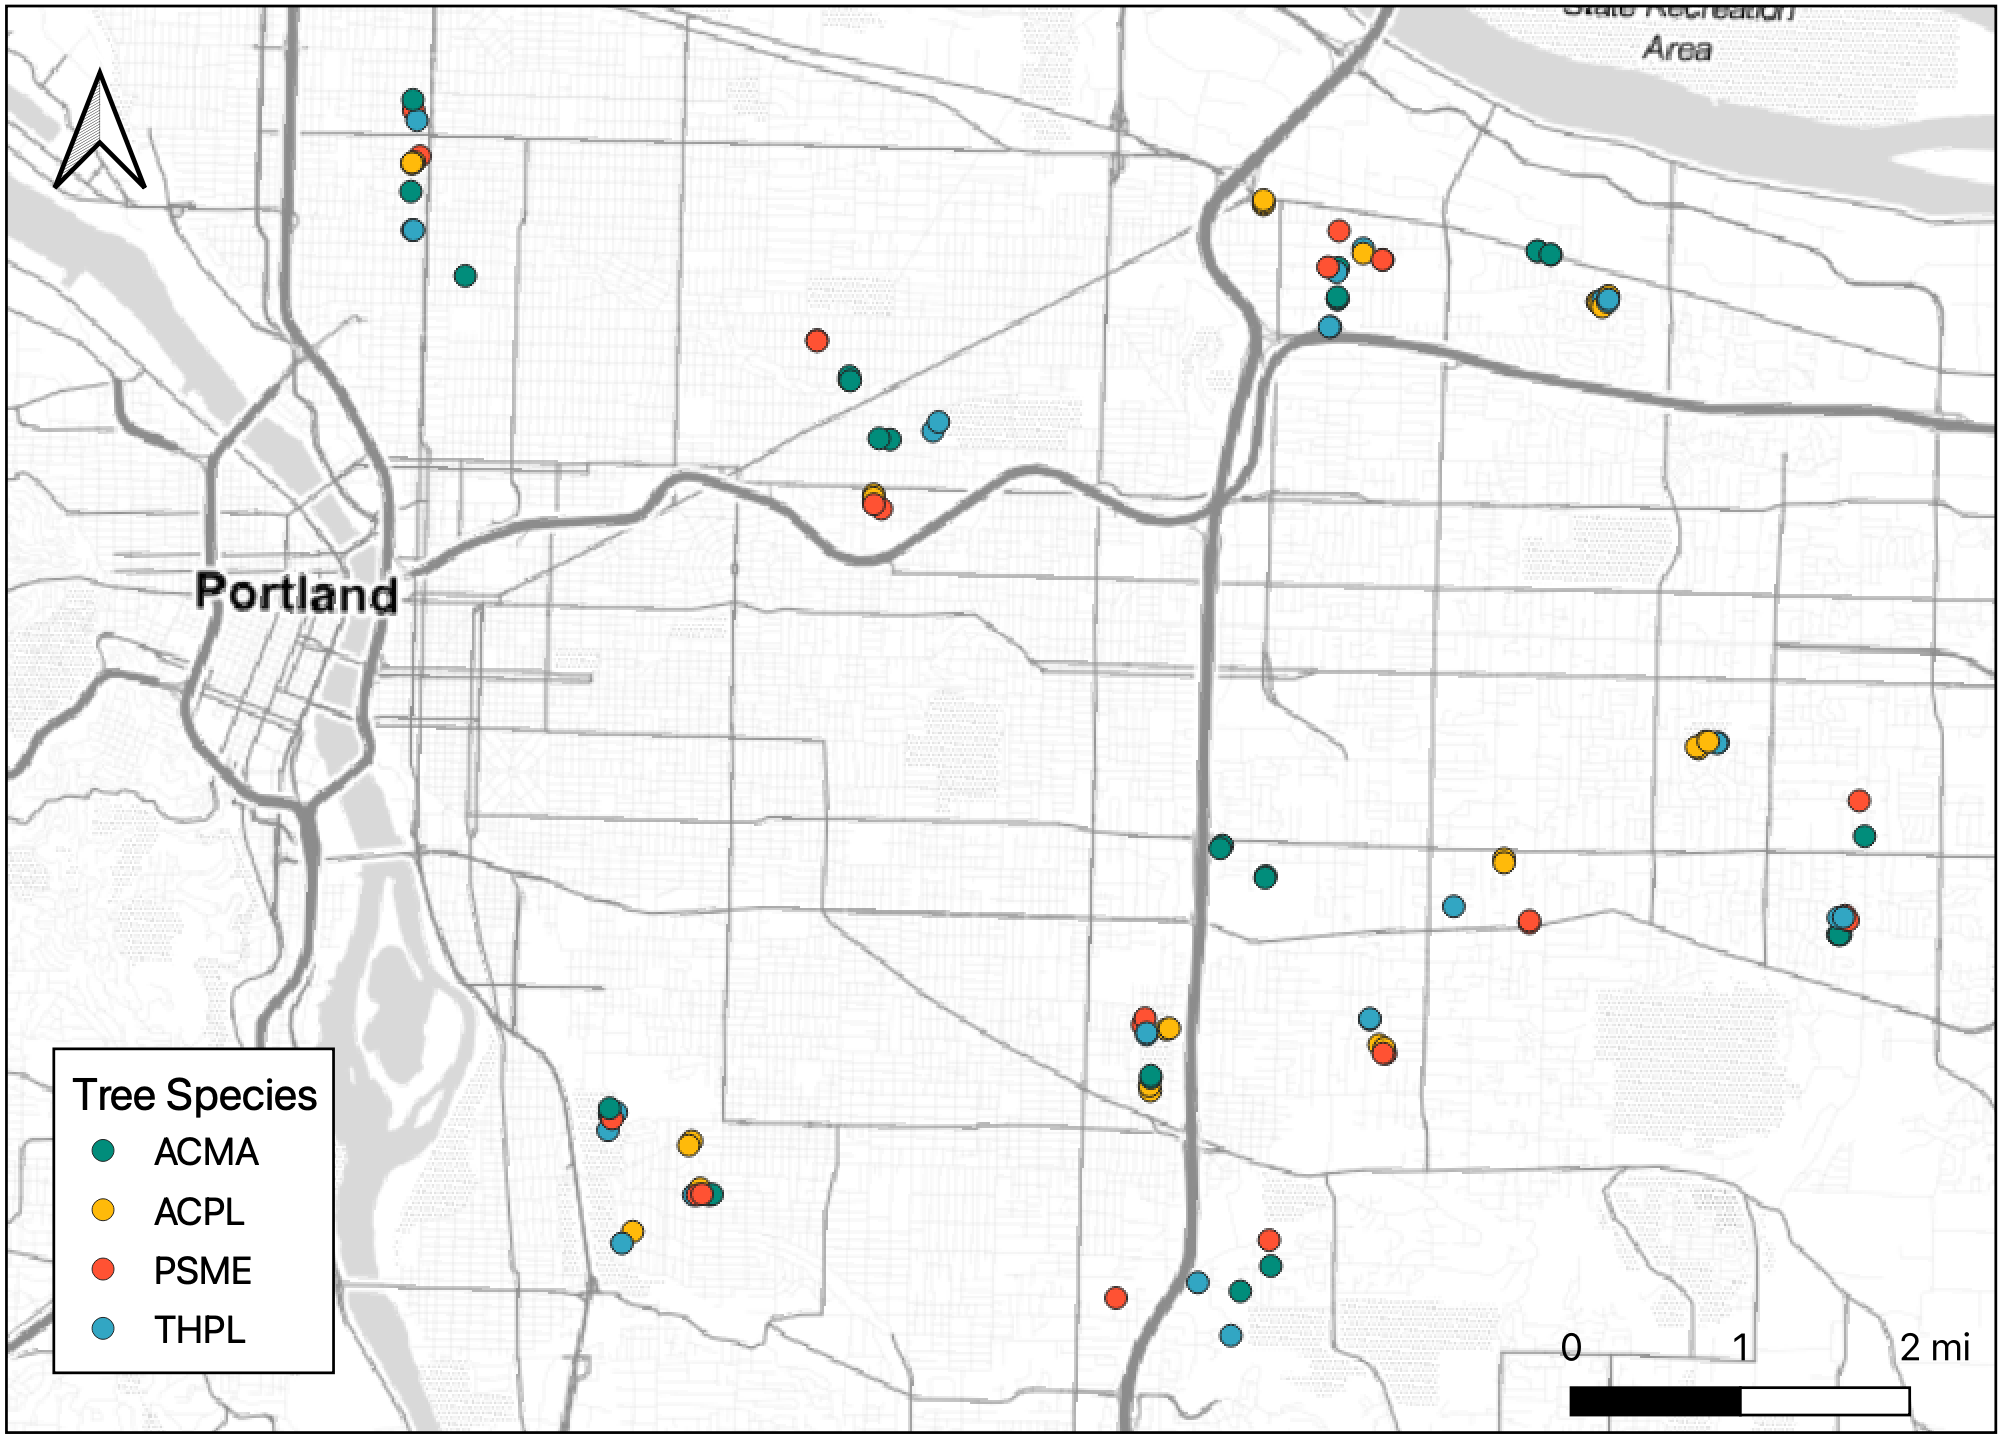
\includegraphics[width=1\linewidth]{figure/cnh_trees} 

}

\caption{Sampled CNH Trees}\label{fig:cnh-trees}
\end{figure}
\hypertarget{portland-tree-inventory}{%
\section{Portland Tree Inventory}\label{portland-tree-inventory}}

The Portland Tree Inventory Project, managed by the City of Portland's Parks \& Recreation Urban Forestry Department, cataloged nearly 245,000 street and park trees in Portland between 2010 to 2019. The street tree inventory, which was collected from 2010 to 2016, contains information on 216,750 street trees of 145 genera. The park tree inventory, collected from 2017 to 2019, contains data on 25,740 park trees of 116 genera. While many of the collected variables differ between the two inventories, they both include data on location, tree identification, DBH, and a visual assessment of the trees health which was rated as good, fair, poor, or dead.

To reduce the variability in data due to the time span of data collection, I filtered the street and park tree inventories to trees that were sampled in 2016 and 2019, respectively. For each dataset, the selected year was the year with the highest count of trees sampled (Tables \ref{tab:streettable} and \ref{tab:parktable}).
\begin{table}

\caption[Species counts in Street Trees Database]{\label{tab:streettable}Species counts in the Portland Street Trees Database}
\centering
\begin{tabular}[t]{llrr}
\toprule
Species code & Scientific name & Collected in 2016 & Total in inventory\\
\midrule
ACPL & Acer platanoides & 4373 & 19209\\
THPL & Thuja plicata & 578 & 1341\\
ACMA & Acer macrophyllum & 1306 & 2609\\
PSME & Pseudotsuga menziesii & 1254 & 3141\\
\bottomrule
\end{tabular}
\end{table}
\begin{table}

\caption[Species counts in Park Trees Database]{\label{tab:parktable}Species counts in the Portland Park Trees Database}
\centering
\begin{tabular}[t]{llrr}
\toprule
Species code & Scientific name & Collected in 2019 & Total in inventory\\
\midrule
ACPL & Acer platanoides & 411 & 1502\\
THPL & Thuja plicata & 331 & 964\\
PSME & Pseudotsuga menziesii & 3237 & 6783\\
ACMA & Acer macrophyllum & 256 & 490\\
\bottomrule
\end{tabular}
\end{table}
The Portland park and street tree inventories include a health categorization variable of Good, Fair, Poor, or Dead. A drawback that can come with qualitative health ratings such as this one is that if a tree does not appear close to death, or perfectly healthy, it is very easy to categorize its health as ``Fair'', which is what we see in both the street and park tree databases. The proportion of trees rated ``Fair'' is extremely high, especially in the park trees inventory (Figure \ref{fig:rating-ratios}).
\begin{figure}
\centering
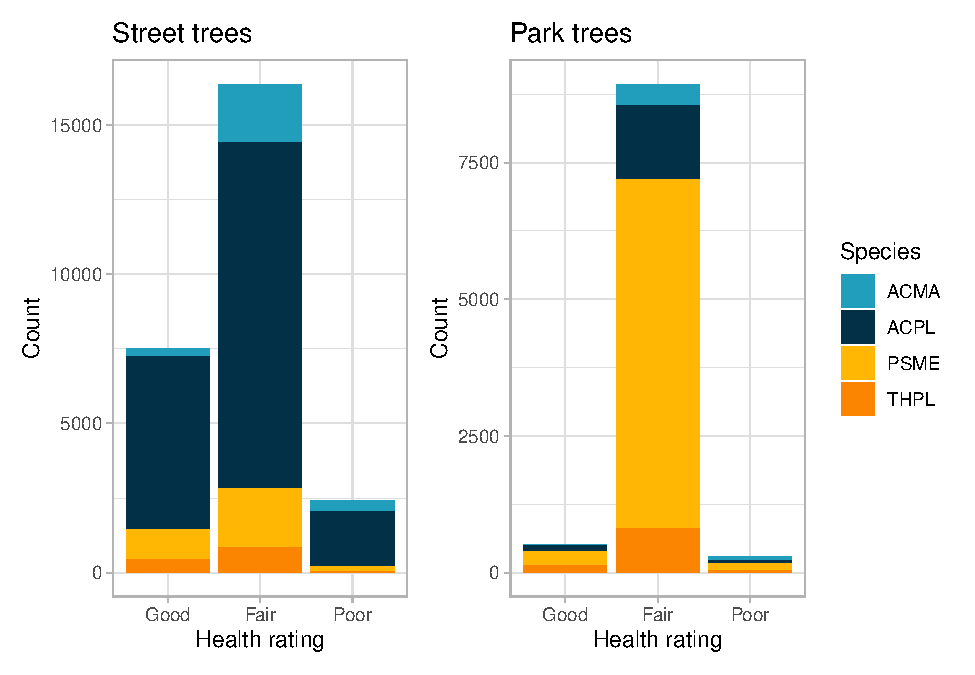
\includegraphics{thesis_files/figure-latex/rating-ratios-1.pdf}
\caption{\label{fig:rating-ratios}Distribution of Health Ratings in the Portland Tree Inventories}
\end{figure}
\hypertarget{canopy-width-and-tree-height-model}{%
\section{Canopy width and tree height model}\label{canopy-width-and-tree-height-model}}

The park tree dataset contains measurements for tree height, canopy width, and DBH, but the street tree dataset only contains measurements for DBH. Canopy width and tree height are both important factors for tree selection and canopy delineation. Using RStudio, I created a statistical model to predict tree height and crown width based on tree DBH and species, in order to be able to use the same pixel selection methods for both the park and street tree inventories.

\hypertarget{satellite-imagery}{%
\section{Satellite Imagery}\label{satellite-imagery}}

PlanetScope satellite imagery (Planet Labs, 3m resolution, 4-band RGB-NIR) was used for vegetation index calculation. PlanetScope, also known as the Flock, is a constellation of approximately 130 satellites . The first 28 PlanetScope satellites were launched in July 2014, and the newest batch of satellites were launched in January 2022. PlanetScope, operated by Planet, is a constellation of approximately 130 satellites, able to image the entire land surface of the Earth every day (a daily collection capacity of 200 million km\(^2\)/day). PlanetScope images are approximately 3 meters per pixel resolution ({``Planet imagery product specifications,''} 2022).

I downloaded satellite images corresponding to the summers of when the data was collected (2016, 2019, and 2021). Images were first filtered for those captured in July of each year, since images taken during the middle of the on-leaf period have been shown to be most sensitive in detecting a statistical difference in tree health measured by NDVI (Fang et al., 2020). The remaining images were then filtered for minimal cloud cover and maximum coverage of the area of study. The final selected images were taken between 6:30 and 7pm on 6 July 2016, 31 July 2019, and 26 July 2021 (Table \ref{tab:sat-products}).
\begin{longtable}[t]{llrl}
\caption{\label{tab:sat-products}Satellite product specifications}\\
\toprule
Collection date & Collection time & Number of scene products & Satellite ID\\
\midrule
2016-07-06 & 18:55 & 5 & 0c22\\
2019-07-31 & 18:42 & 4 & 0f42\\
2021-07-26 & 18:40 & 4 & 1003\\
\bottomrule
\end{longtable}
For each of the chosen dates, I downloaded the available analytic product from Planet. The analytic multispectral imagery products are orthorectified, calibrated, corrected for terrain distortions, and transformed to Top of Atmosphere radiance to ensure accurate geolocation and cartographic projection.

The bands in a saptellite product refer to the reflectance wavelength that is picked up by the satellite. For a 4-band satellite product, the wavelengths are split into red, green, blue, and near-infrared (NIR) bands (Table \ref{tab:wavelength}). In the raw PlanetScope product, these 4 bands come compressed in one .tif image. In order to extract NDVI data from the imagery products, the data requires further processing.
\begin{longtable}[t]{ll}
\caption[4-band satellite wavelength ranges]{\label{tab:wavelength}Wavelength ranges for 4-band Planetscope satellite bands}\\
\toprule
Band name & Wavelength range\\
\midrule
Blue & 455 - 515 nm\\
Green & 500 - 590 nm\\
Red & 590 - 670 nm\\
NIR & 780 - 860 nm\\
\bottomrule
\end{longtable}
\hypertarget{ndvi-calculation}{%
\section{NDVI calculation}\label{ndvi-calculation}}

The NDVI calculations were done using Python in PyCharm. Besides minor alterations, the processing code came from Planet's instructions on calculating NDVI from 4-band PlanetScope data (Planet, n.d.). NDVI is calculated from the red and NIR satellite bands, as shown in Equation \eqref{eq:ndvi-eq}.
\begin{equation}
  \mathrm{NDVI} = \frac{(NIR - Red)}{(NIR + Red)} 
  \label{eq:ndvi-eq}
\end{equation}
\begin{figure}

{\centering 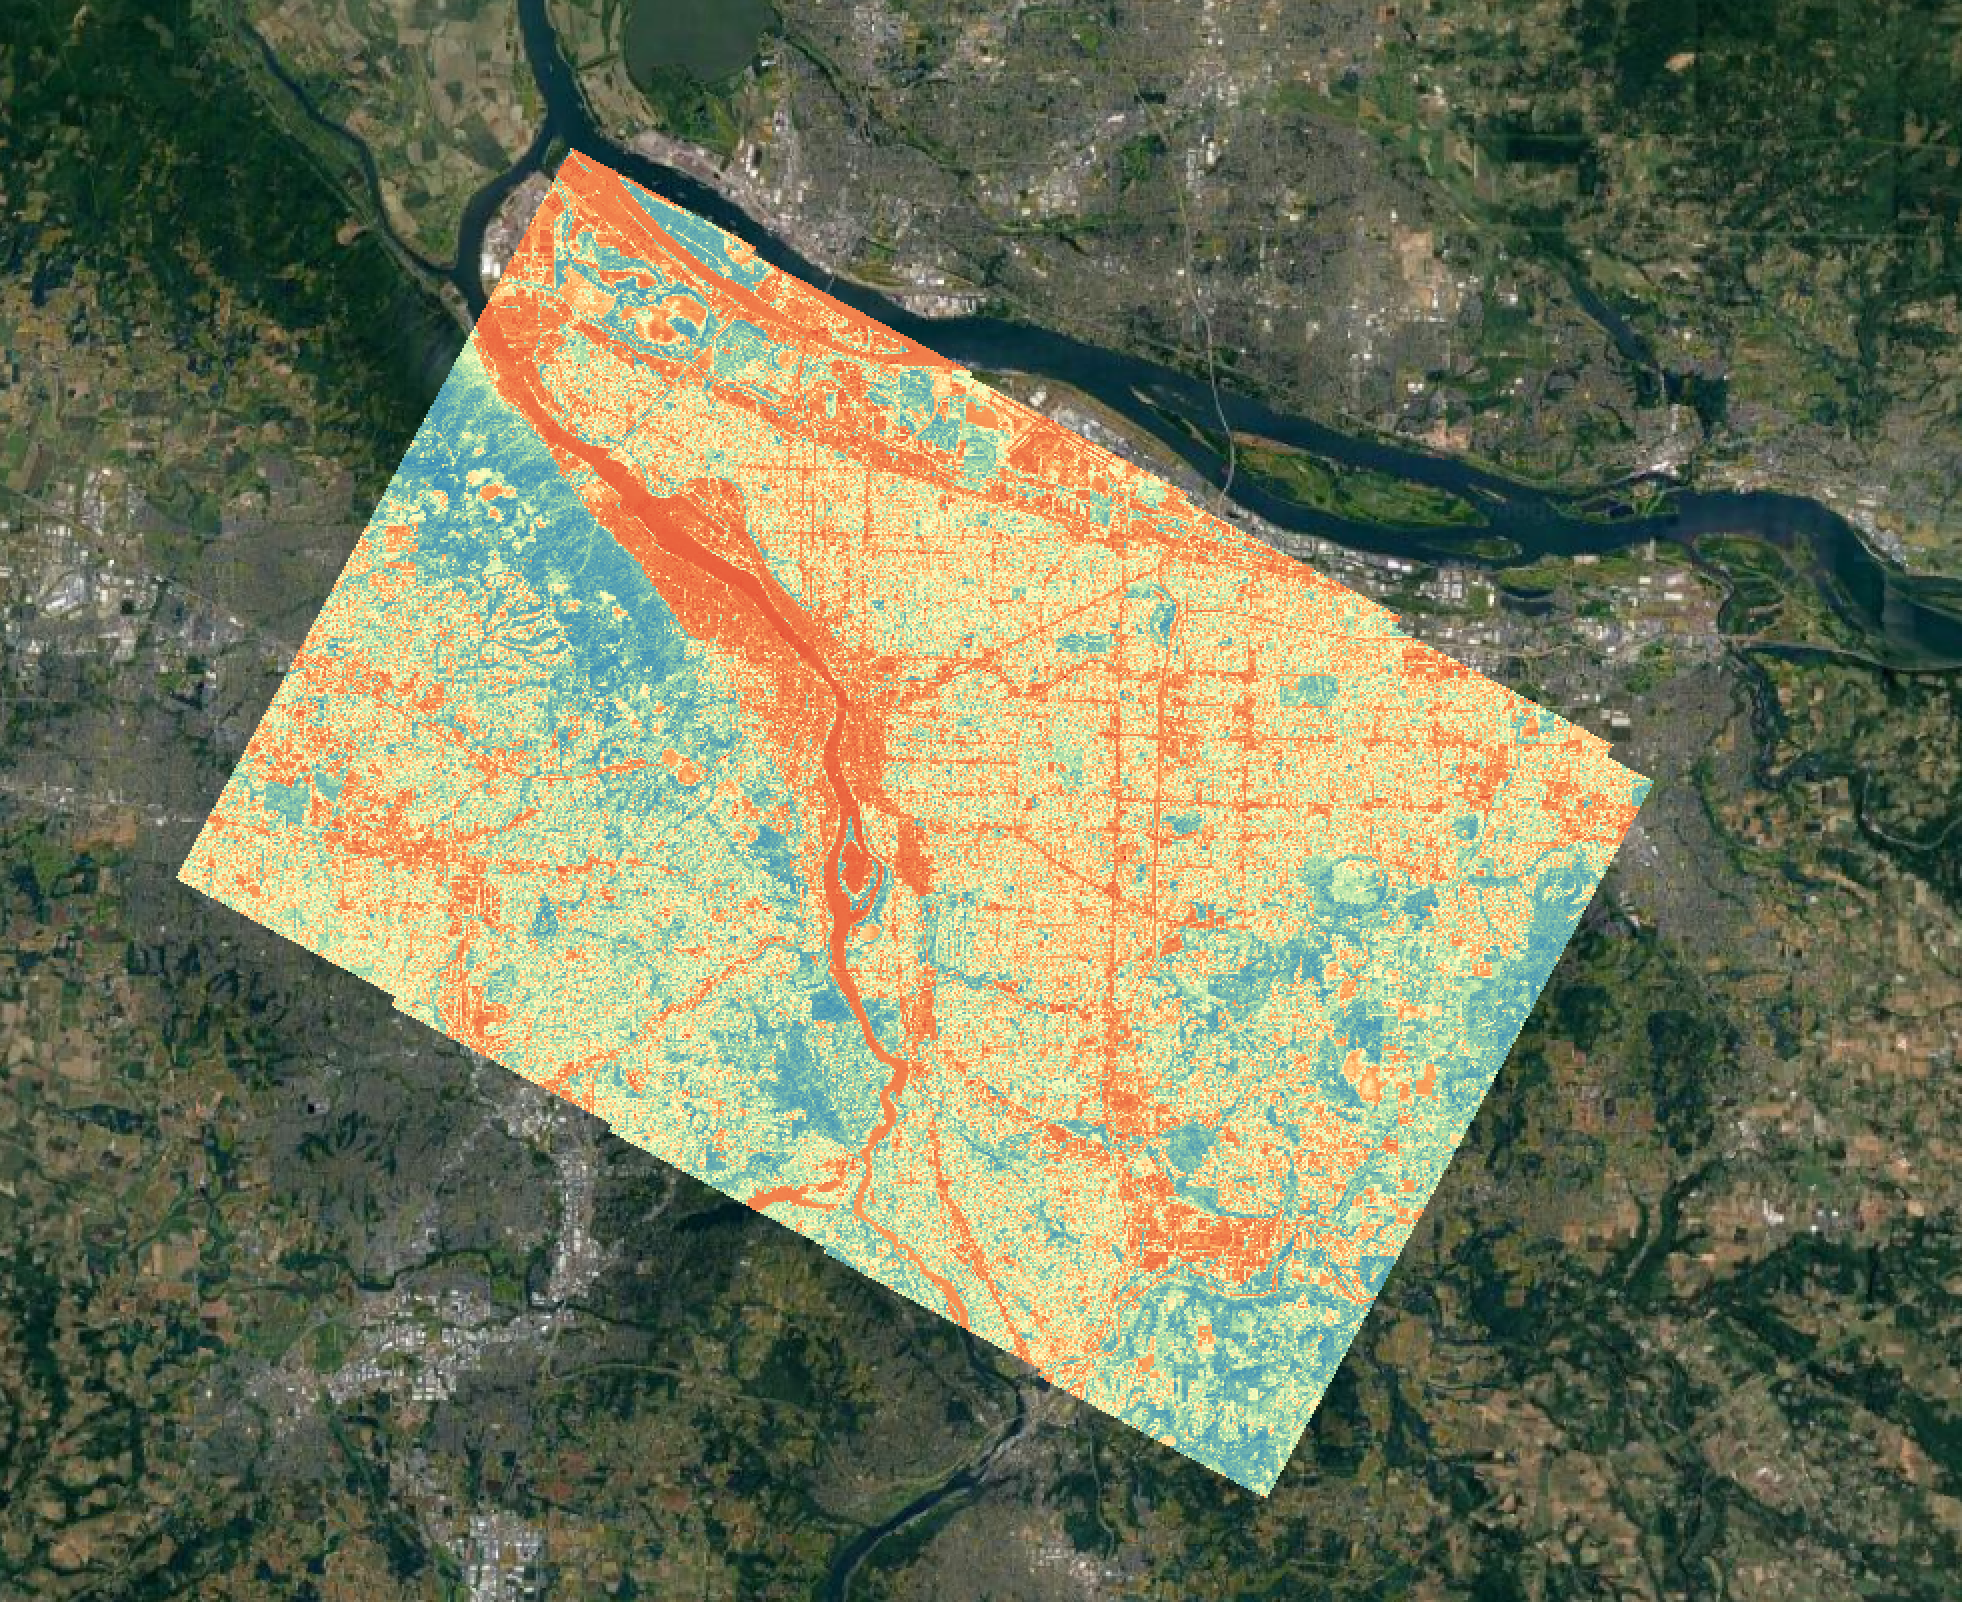
\includegraphics[width=0.32\linewidth]{figure/2016_ndvi} 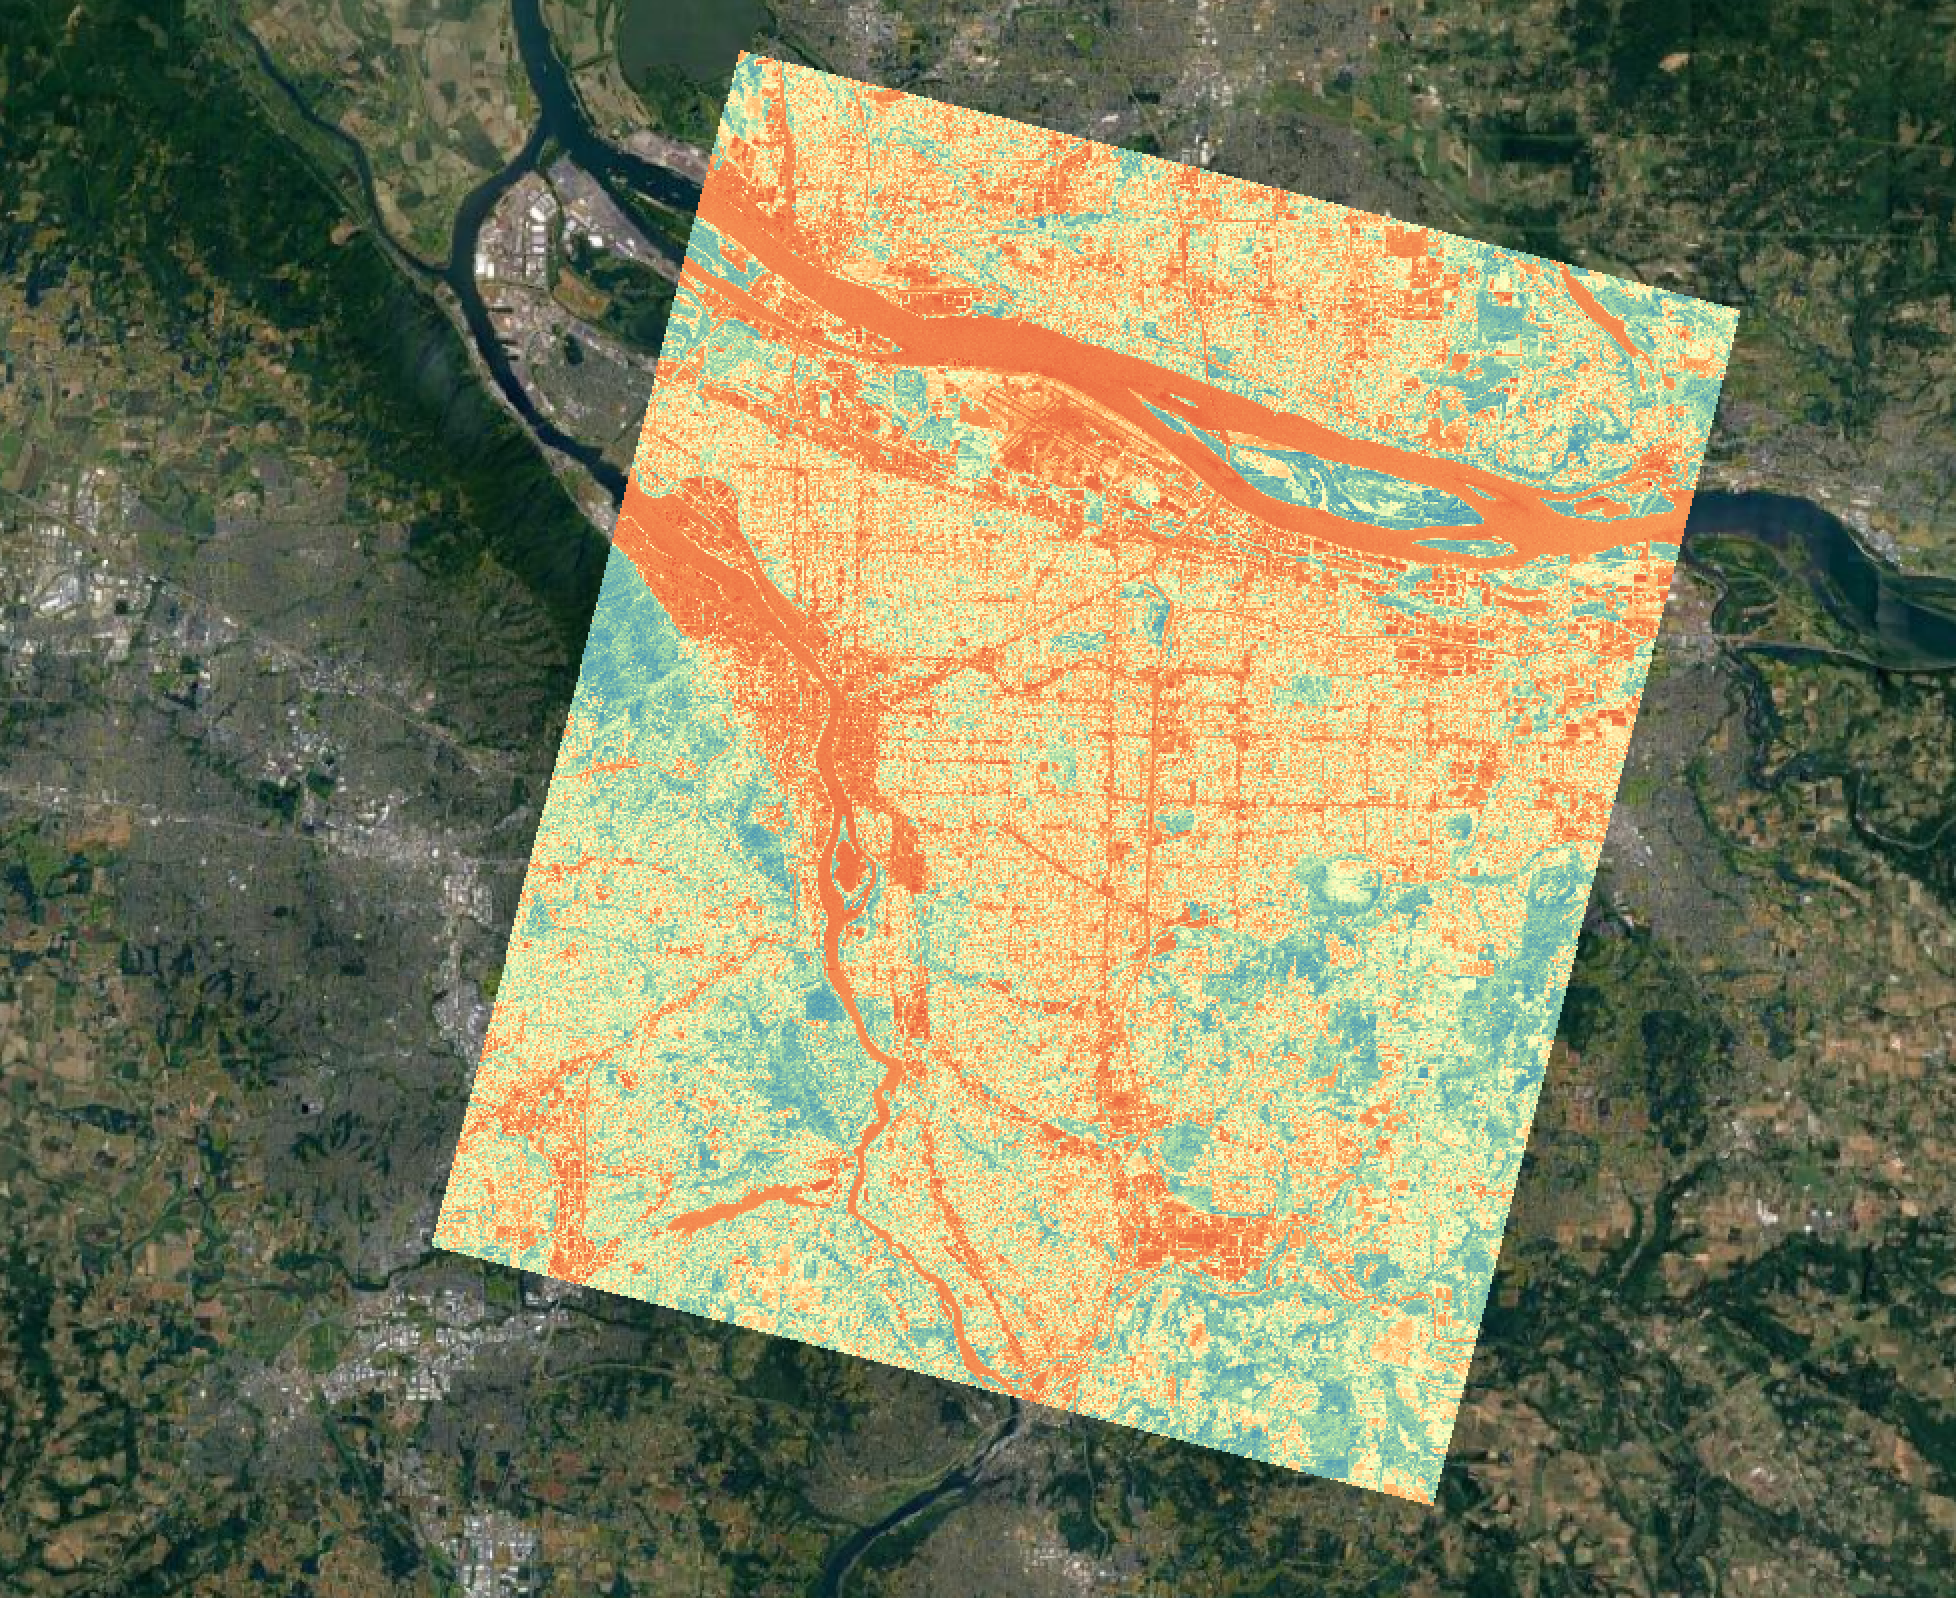
\includegraphics[width=0.32\linewidth]{figure/2019_ndvi} 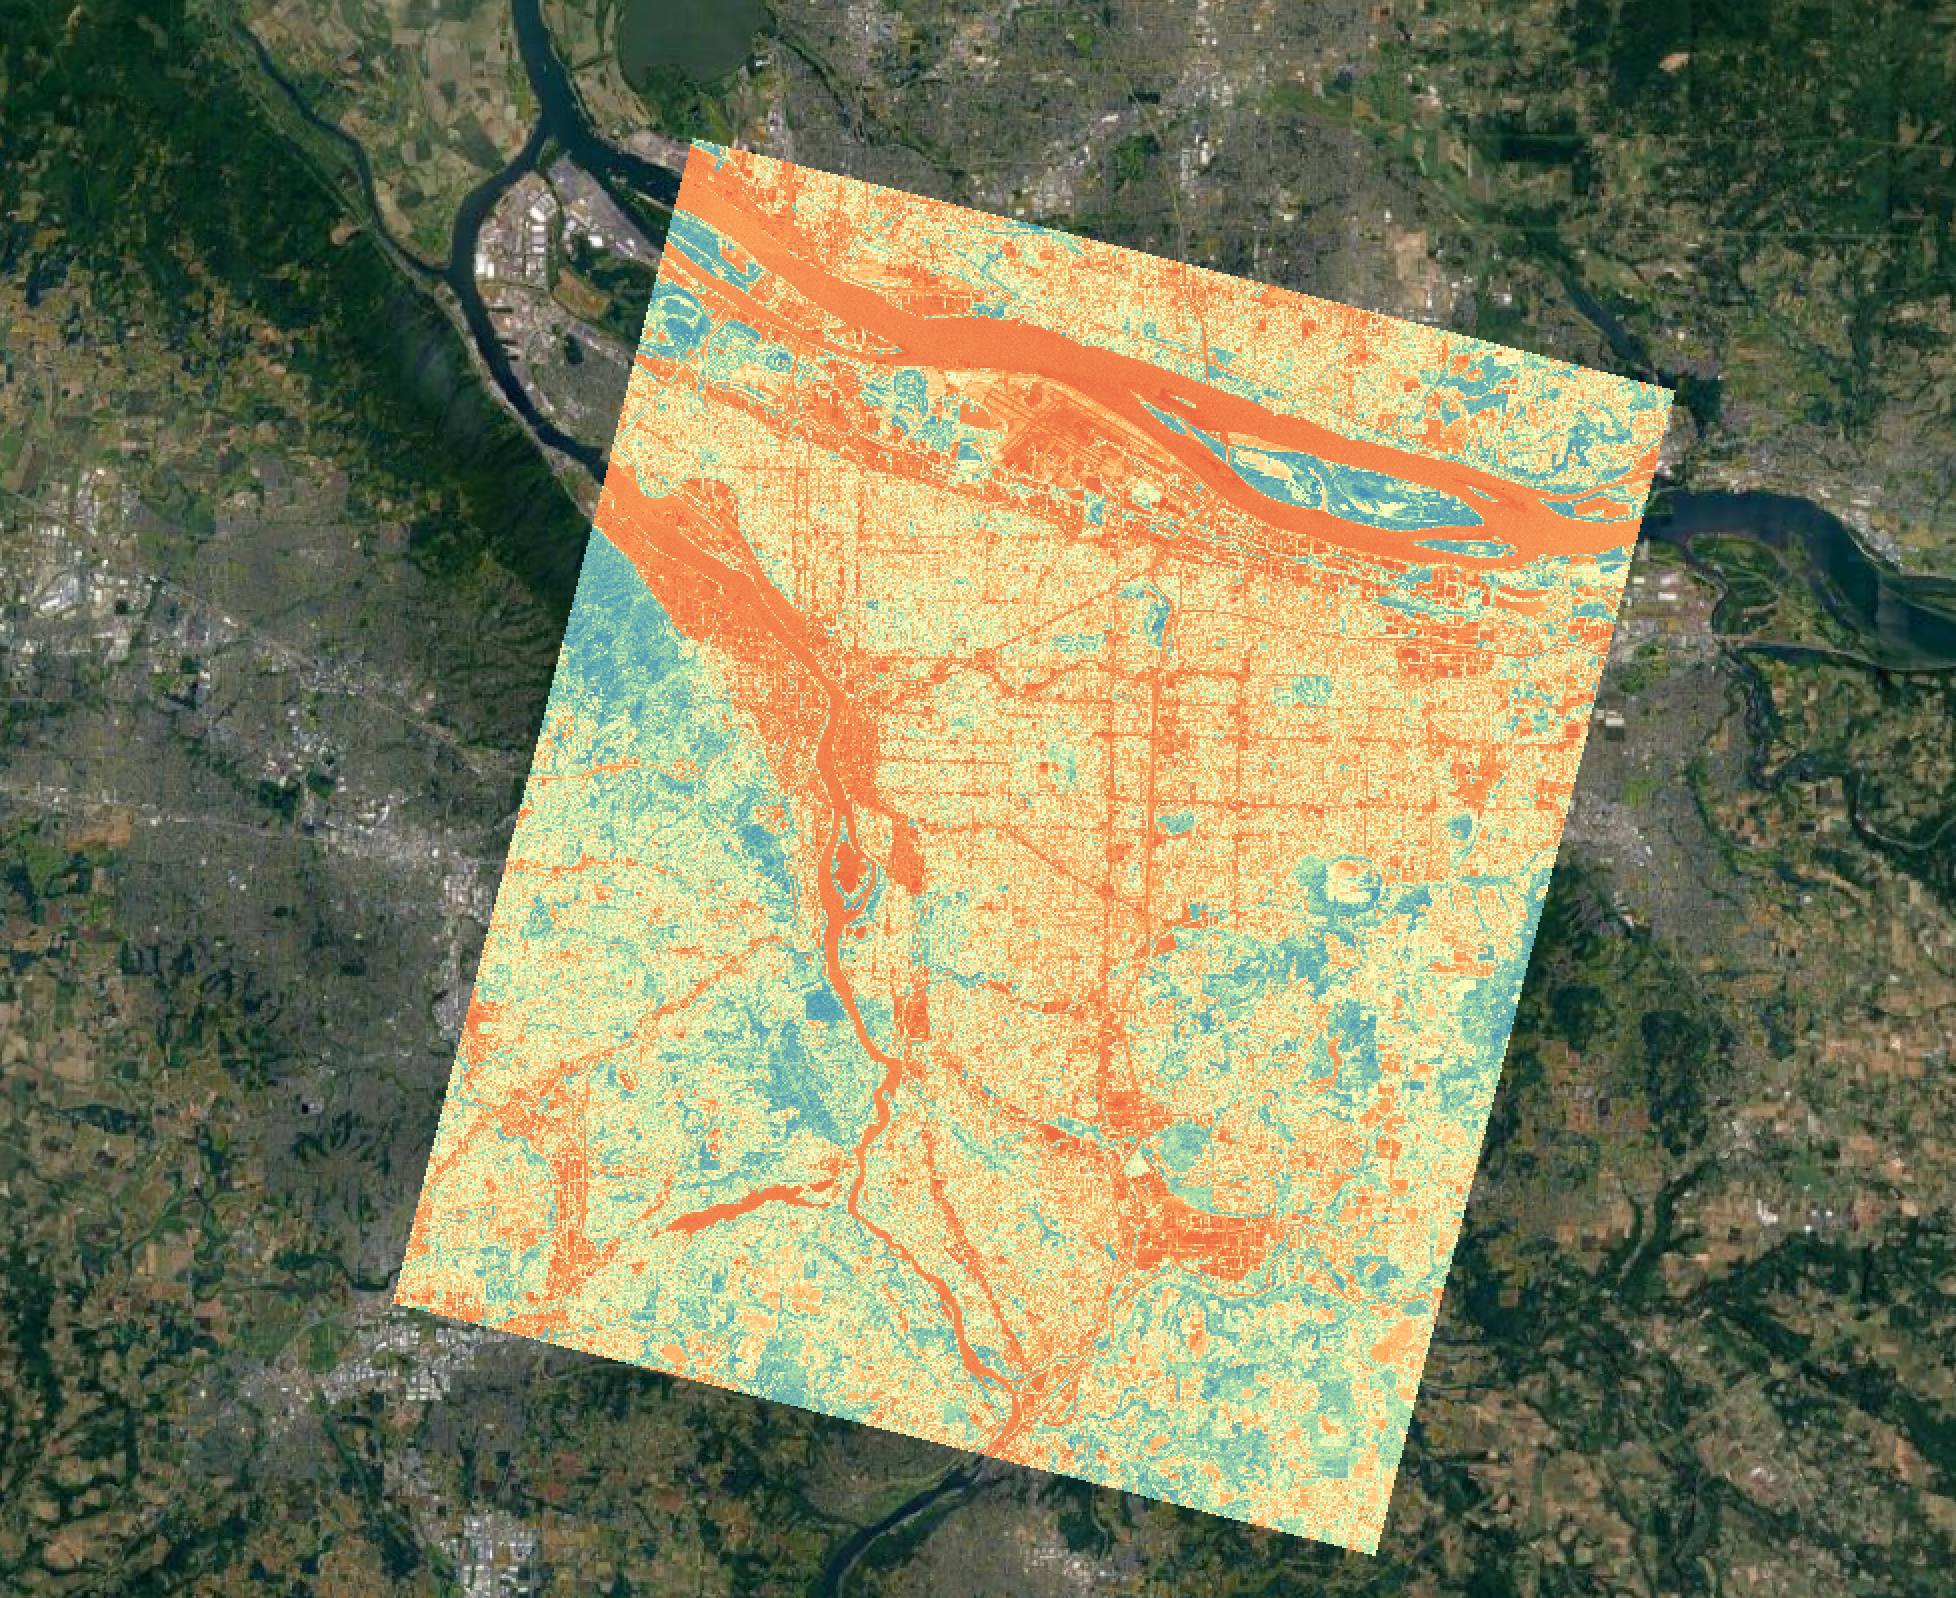
\includegraphics[width=0.32\linewidth]{figure/2021_ndvi} 

}

\caption{Product areas for 2016, 2019, and 2021 satellite scenes}\label{fig:areafigs}
\end{figure}
\hypertarget{chm}{%
\section{Canopy Height Model}\label{chm}}

A canopy height model for the Portland metro area was developed using LiDAR and satellite spectral imagery collected in the summer of 2014 ({``Canopy 2014,''} 2016). The purpose of this data is to monitor natural areas in the Portland metro area, specifically change over time analysis and the examination of the potential loss of habitat in riparian areas. The canopy was detected using both NDVI values and LiDAR feature heights. Errors and noise in the data, such as electrical lines above tree tops, were cleaned using geometric post-processing. The canopy height model was clipped to remove anything below ten feet to eliminate any understory shrubs or grasses that were included in the raw data ({``Canopy 2014,''} 2016).

\hypertarget{tree-crown-delineation-and-pixel-selection}{%
\section{Tree Crown Delineation and Pixel Selection}\label{tree-crown-delineation-and-pixel-selection}}

The goal of tree crown delineation is to understand where the foliage of a tree is located. This is extremely important because we want to ensure that the satellite pixels used for health analysis have measurements that belong to the given tree. Previous papers such as have used manual tree crown delineation (Xiao \& McPherson, 2005), or chosen a standardized radius for all trees in their sample (Fang et al., 2020). Manual tree crown delineation would be extremely time consuming, especially when trying to examine data on a city-wide level. Additionally, with a standardized radius, there will be many trees that have crowns either larger or smaller than the standardized radius. If the true crown is smaller than that of the radius, pixels that correspond to things like grass or pavement will be included in the measurement analysis. Conversely, if the true crown is larger than the chosen radius, the edges of the tree will be ignored, and valuable data will be lost. With both of these methods, any overlapping tree crowns were removed from the final analysis, even further reducing the sample size.

In this thesis, I test three different methods of pixel selection for NDVI analysis. First, I test a ``point method'' which uses the NDVI value directly below an inventoried trees location point. Second, I use crown width measurements and predictions to create a variable radius method, and average the NDVI pixels within the created circle. Lastly, I use a LiDAR created canopy height model for Portland's urban canopy with \texttt{ForestTools} canopy delineation algorithm to create canopy polygons for NDVI analysis.

For the following examples, I use Berkeley Park, located in SE Portland, to demonstrate the different delineation techniques. We sampled 6 CNH trees in Berkeley Park: 2 Bigleaf Maple, 1 Norway Maple, 2 Douglas Fir, and 1 Western Redcedar (Figure \ref{fig:berkeley-park}).
\begin{figure}

{\centering 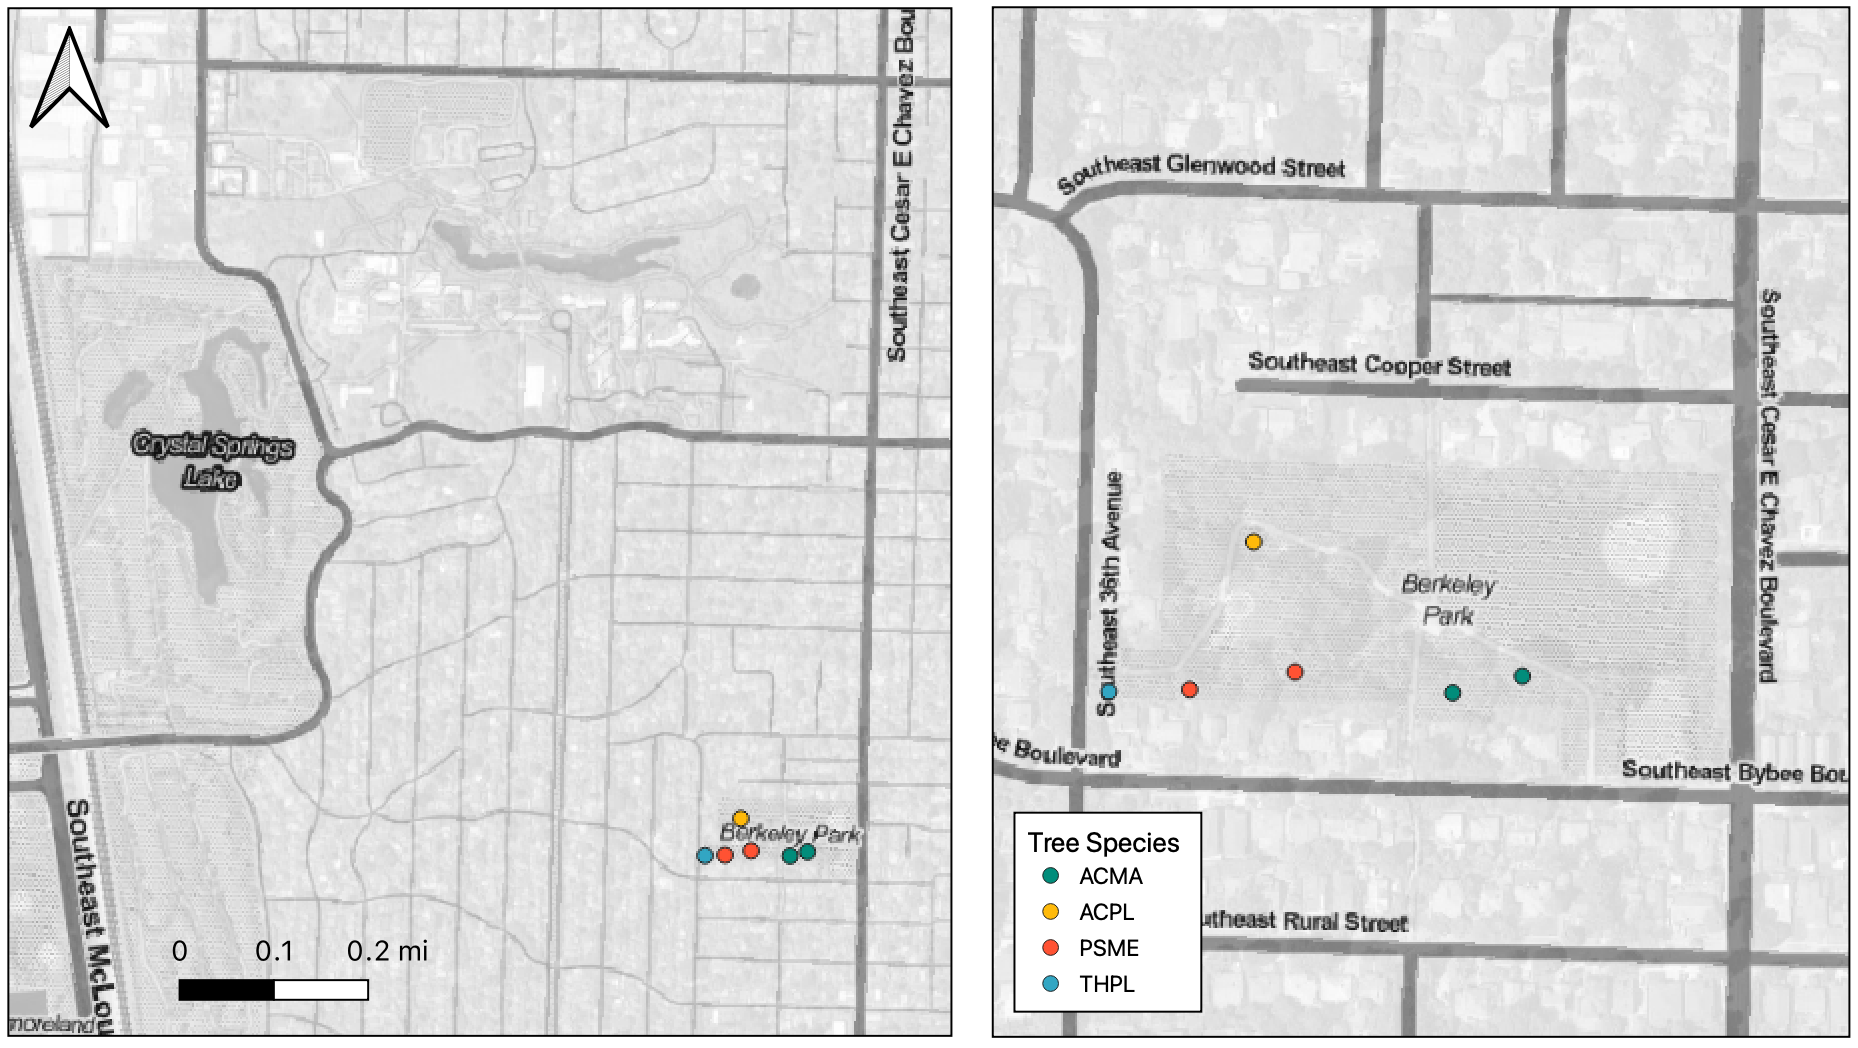
\includegraphics[width=1\linewidth]{figure/berkeley_park} 

}

\caption{Berkeley Park and CNH trees}\label{fig:berkeley-park}
\end{figure}
\hypertarget{point-method}{%
\subsection{Point method}\label{point-method}}

Point Method: For the point method, I extracted the NDVI value from the pixel directly underneath the tree location point. This is the simplest of the three methods, since it obtains one NDVI value for one singular pixel. The tree location points were sourced from the street and park tree inventories and processed in QGIS (Figure \ref{fig:point-method}). The main source of potential error with this technique is with the tree point location. If the point was placed incorrectly, the NDVI value will not be representative of the tree's greenness, or health.
\begin{figure}

{\centering 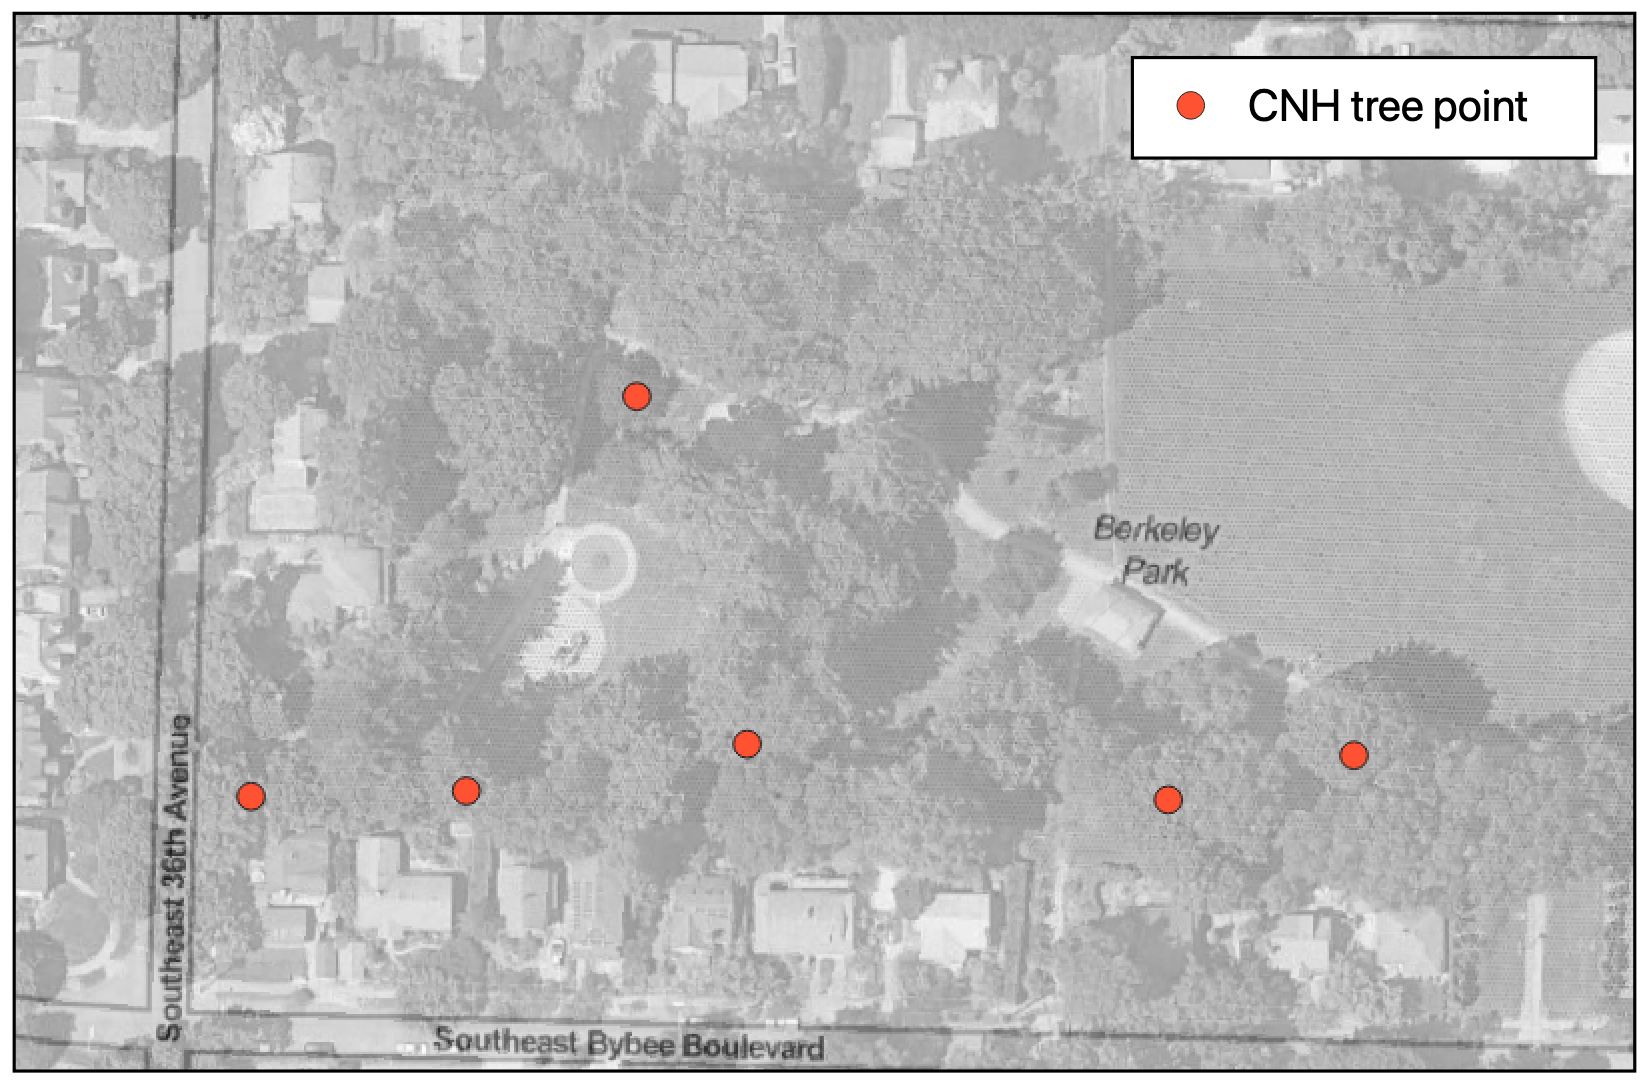
\includegraphics[width=0.8\linewidth]{figure/points} 

}

\caption{CNH trees sampled in Berkeley Park}\label{fig:point-method}
\end{figure}
\hypertarget{radius-method}{%
\subsection{Radius method}\label{radius-method}}

The first method of tree crown delineation I used is based on the individual crown width for each selected tree. In the Portland park tree inventory, crown width is measured as an east to west diameter, and a north to south diameter. To get the radius for the buffer, I took the average of both measurements and divided it by 2. For the Portland street tree inventory, crown width was not collected. I used the tree height and crown width predictive model to create crown width measurements. For each selected tree point, I created a buffer with the radius of the measured or predicted tree canopy using QGIS (Figure \ref{fig:point-radius}). To get NDVI for each tree in this method, I averaged the value of all pixels in the buffer circle for each tree using QGIS.

With the radius method, it involves the same risk as the point method that if the central point is incorrectly located, the values will not be representative. Additionally, average NDVI ratings obtained with this method for trees with overlapping crowns will contain NDVI pixels that belong to other trees. Previous studies have removed all overlapping tree crowns when using a radius technique, but that can severely limit sample size of available data for analysis, since especially in urban areas and on streets, most of the trees will have overlapping crowns.
\begin{figure}

{\centering 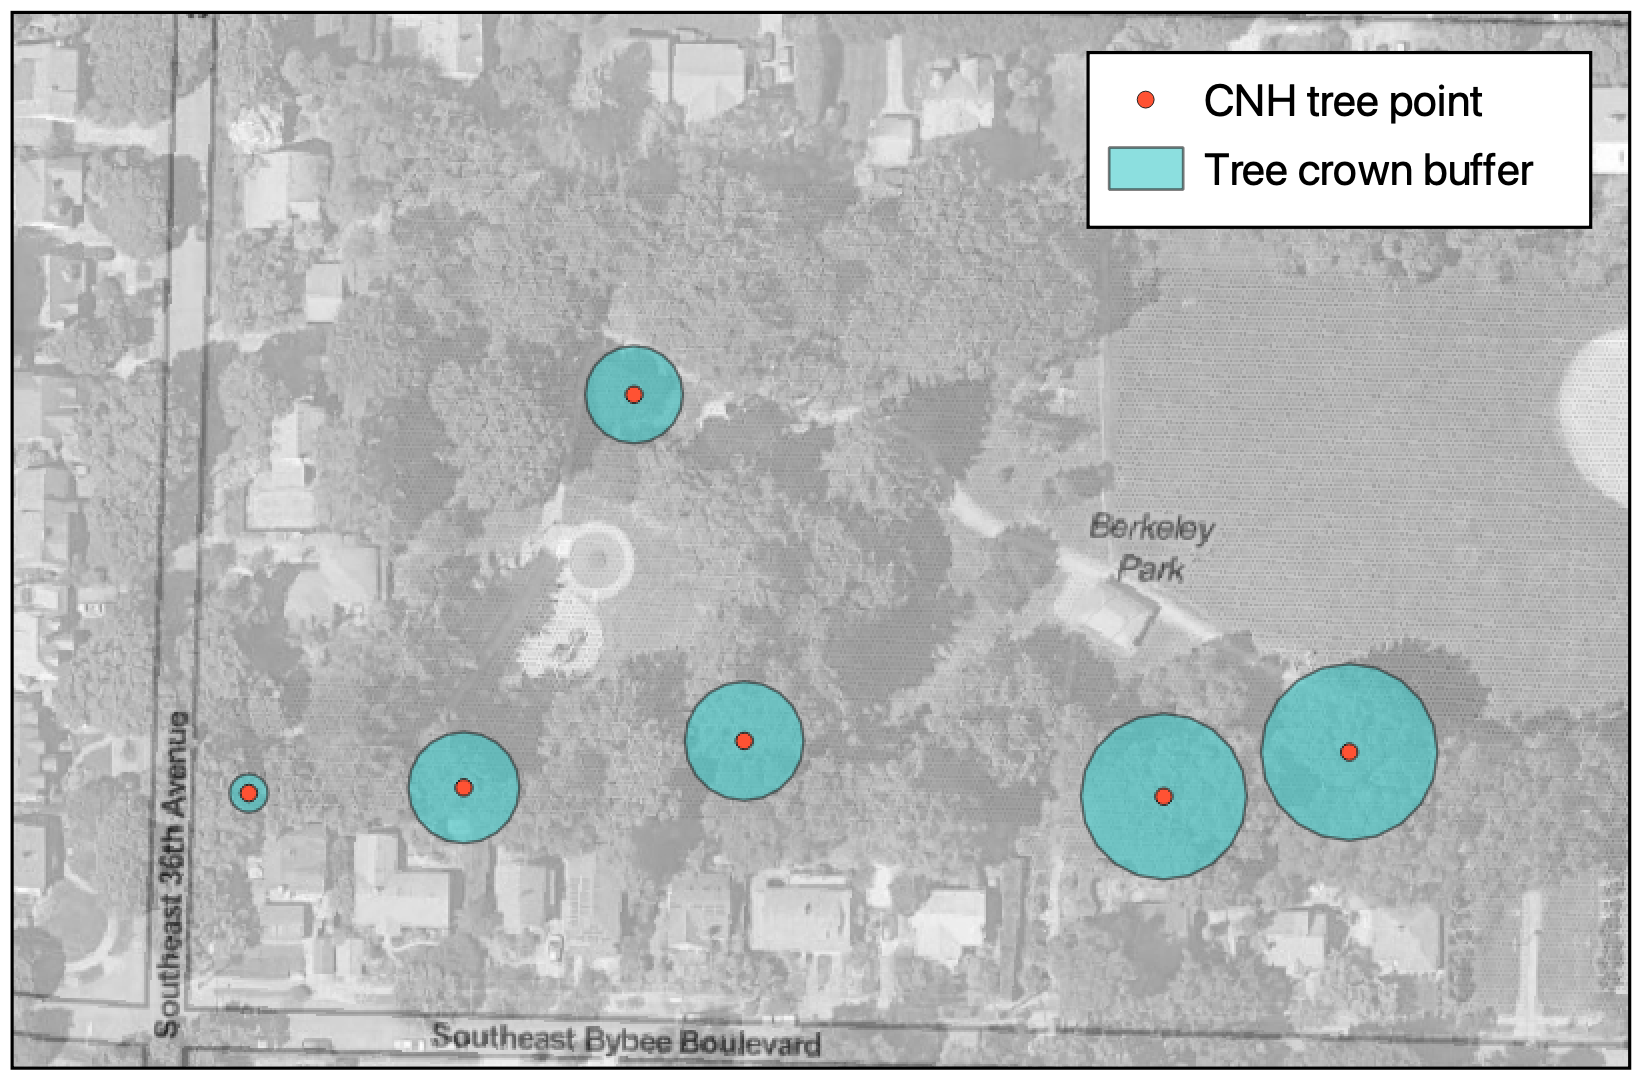
\includegraphics[width=0.8\linewidth]{figure/point_radius} 

}

\caption{CNH trees with crown width buffer}\label{fig:point-radius}
\end{figure}
\hypertarget{lidar-method}{%
\subsection{LiDAR method}\label{lidar-method}}

The LiDAR method is the most complex and involved of the three tree crown delineation methods but has the potential to be the most precise.

The \texttt{ForestTools} crown delineation algorithm is a modified watershed delineation algorithm that takes a LiDAR file input, as well as treetop location point file and outputs a polygon file with predicted tree crowns. \texttt{ForestTools} also has the ability to predict treetop location points based on LiDAR data, but that functionality introduced a lot of error in my processing because it became difficult to re-associate predicted treetop points with the actual tree location points that I was analyzing.

The LiDAR canopy height model was clipped to a 30 meter buffer around each selected tree point to reduce file size in the delineation processing (Figure \ref{fig:lidar-buffer}). A 30m buffer was chosen to ensure that no part of the tree canopy would be omitted from the processing, and to include any near neighboring trees that may have canopy that overlaps with the tree of interest. In order for the algorithm to delineate tree crowns, it needs both LiDAR canopy data and location points for the potential trees for delineation. With a smaller buffer radius, the locations of neighboring trees would be omitted and the canopy delineation algorithm would compute a tree crown as much bigger than it actually is.

With the 30m buffer, all other inventoried trees that are contained within the buffer were selected for inclusion as treetop location points in addition to the trees of interest (Figure \ref{fig:buffer-points}). A minimum tree height of 20 feet was included in the algorithm options but since all sampled trees were already filtered for height requirements, this may not be necessary.
\begin{figure}

{\centering 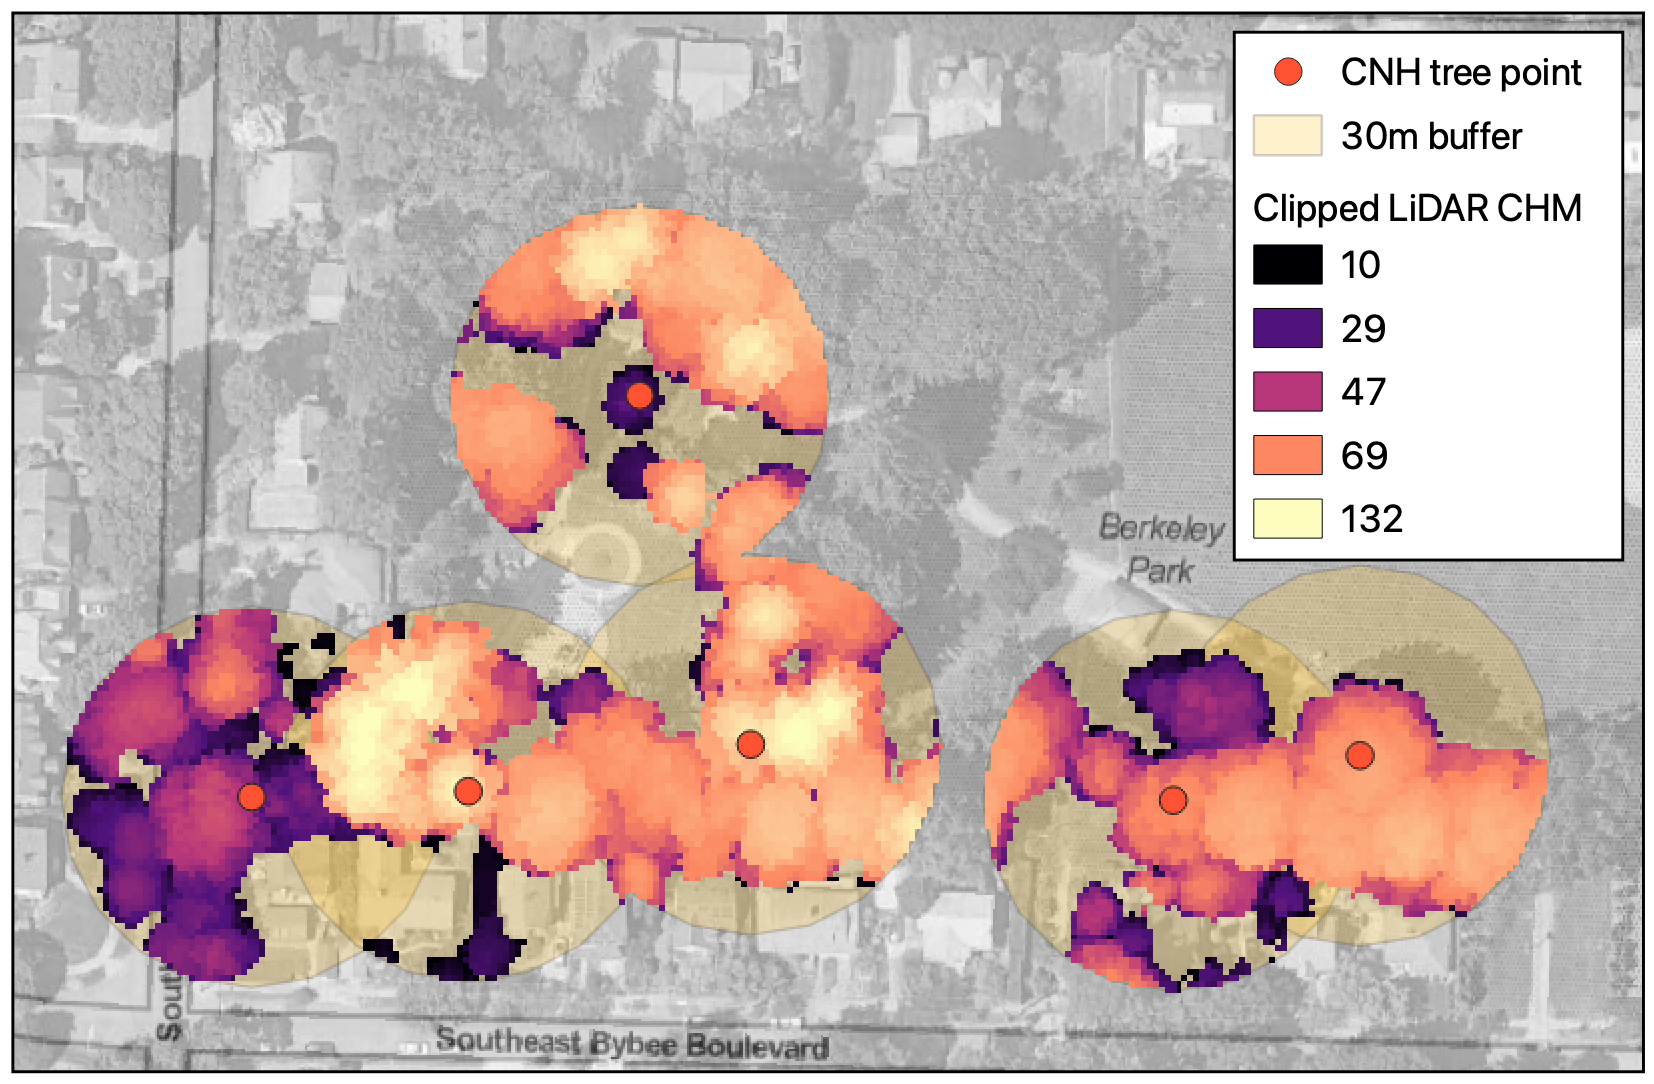
\includegraphics[width=0.8\linewidth]{figure/lidar_buffer_scale} 

}

\caption{LiDAR data clipped to 30m tree buffer}\label{fig:lidar-buffer}
\end{figure}
\begin{figure}

{\centering 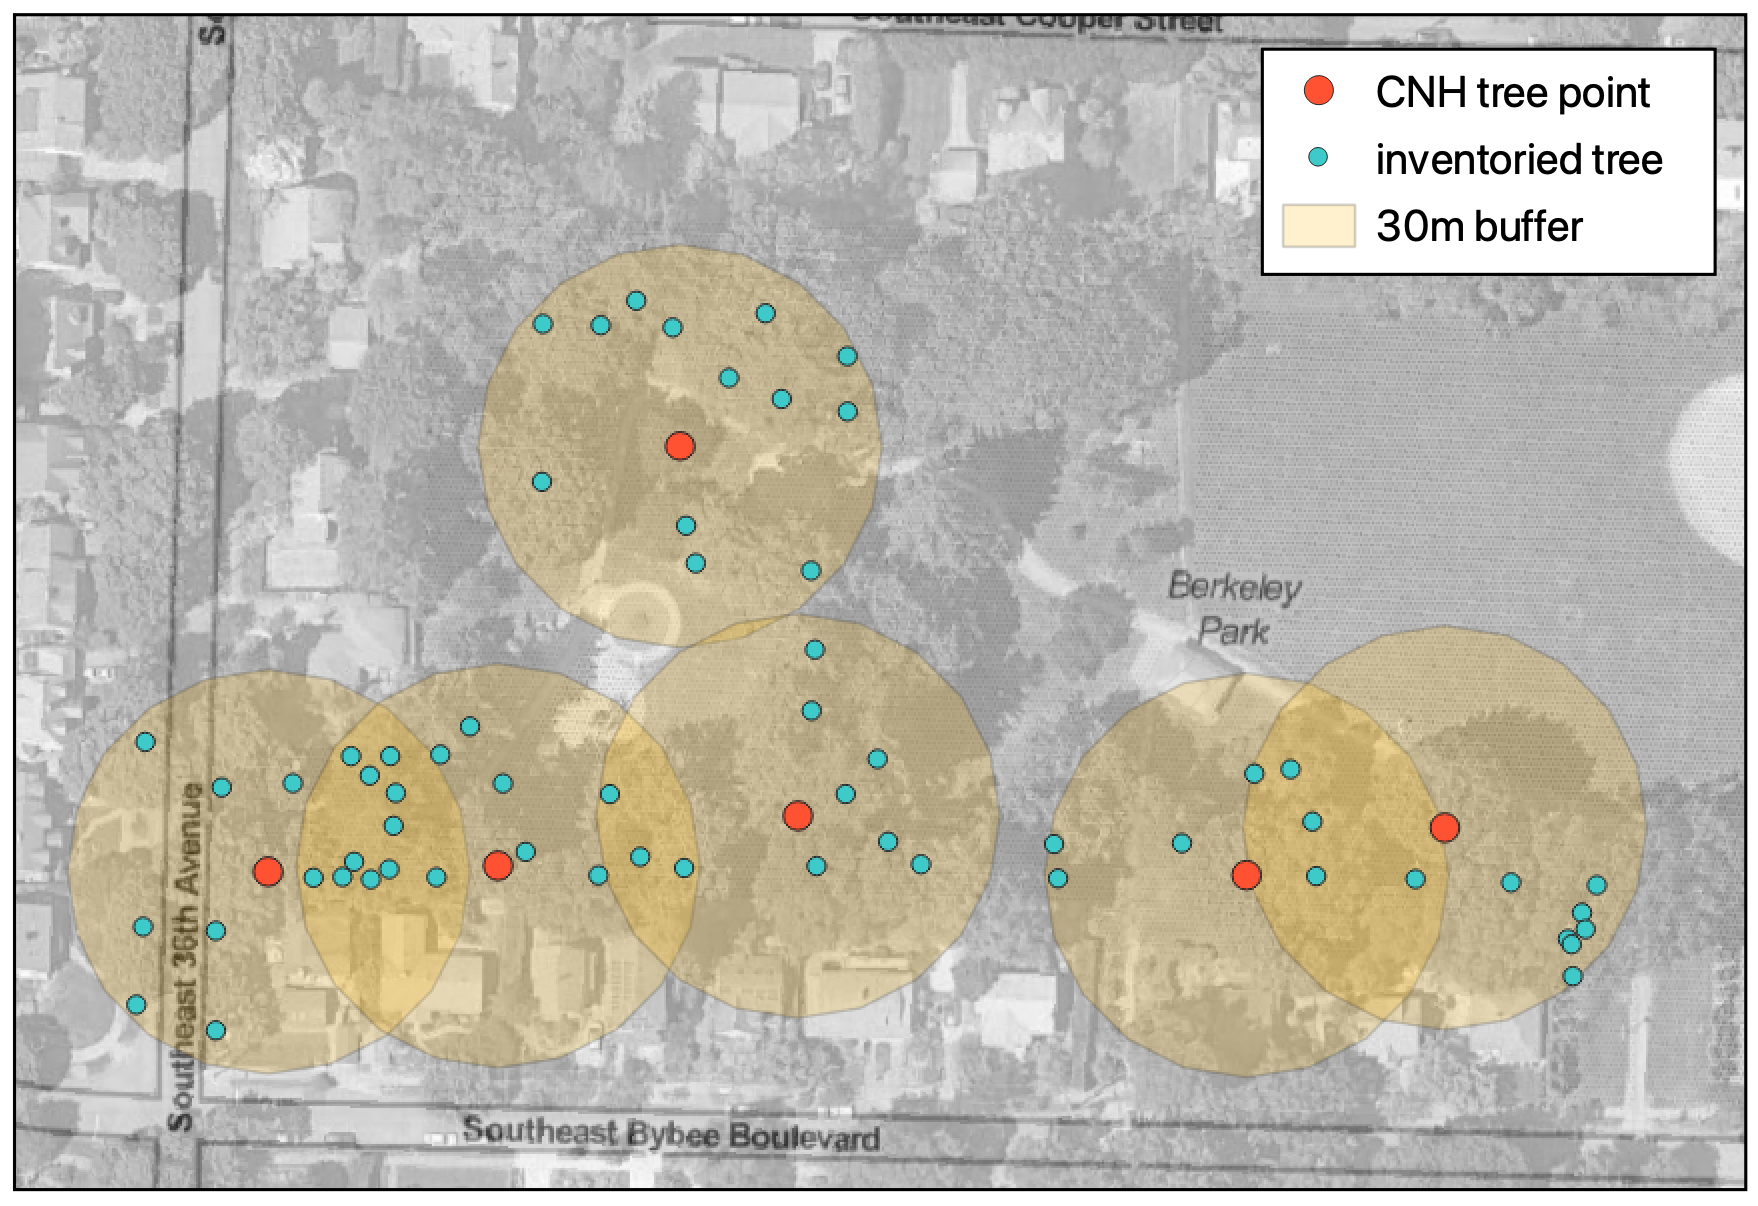
\includegraphics[width=0.8\linewidth]{figure/buffer_all_points} 

}

\caption{All inventoried trees within the 30m buffer}\label{fig:buffer-points}
\end{figure}
\begin{figure}

{\centering 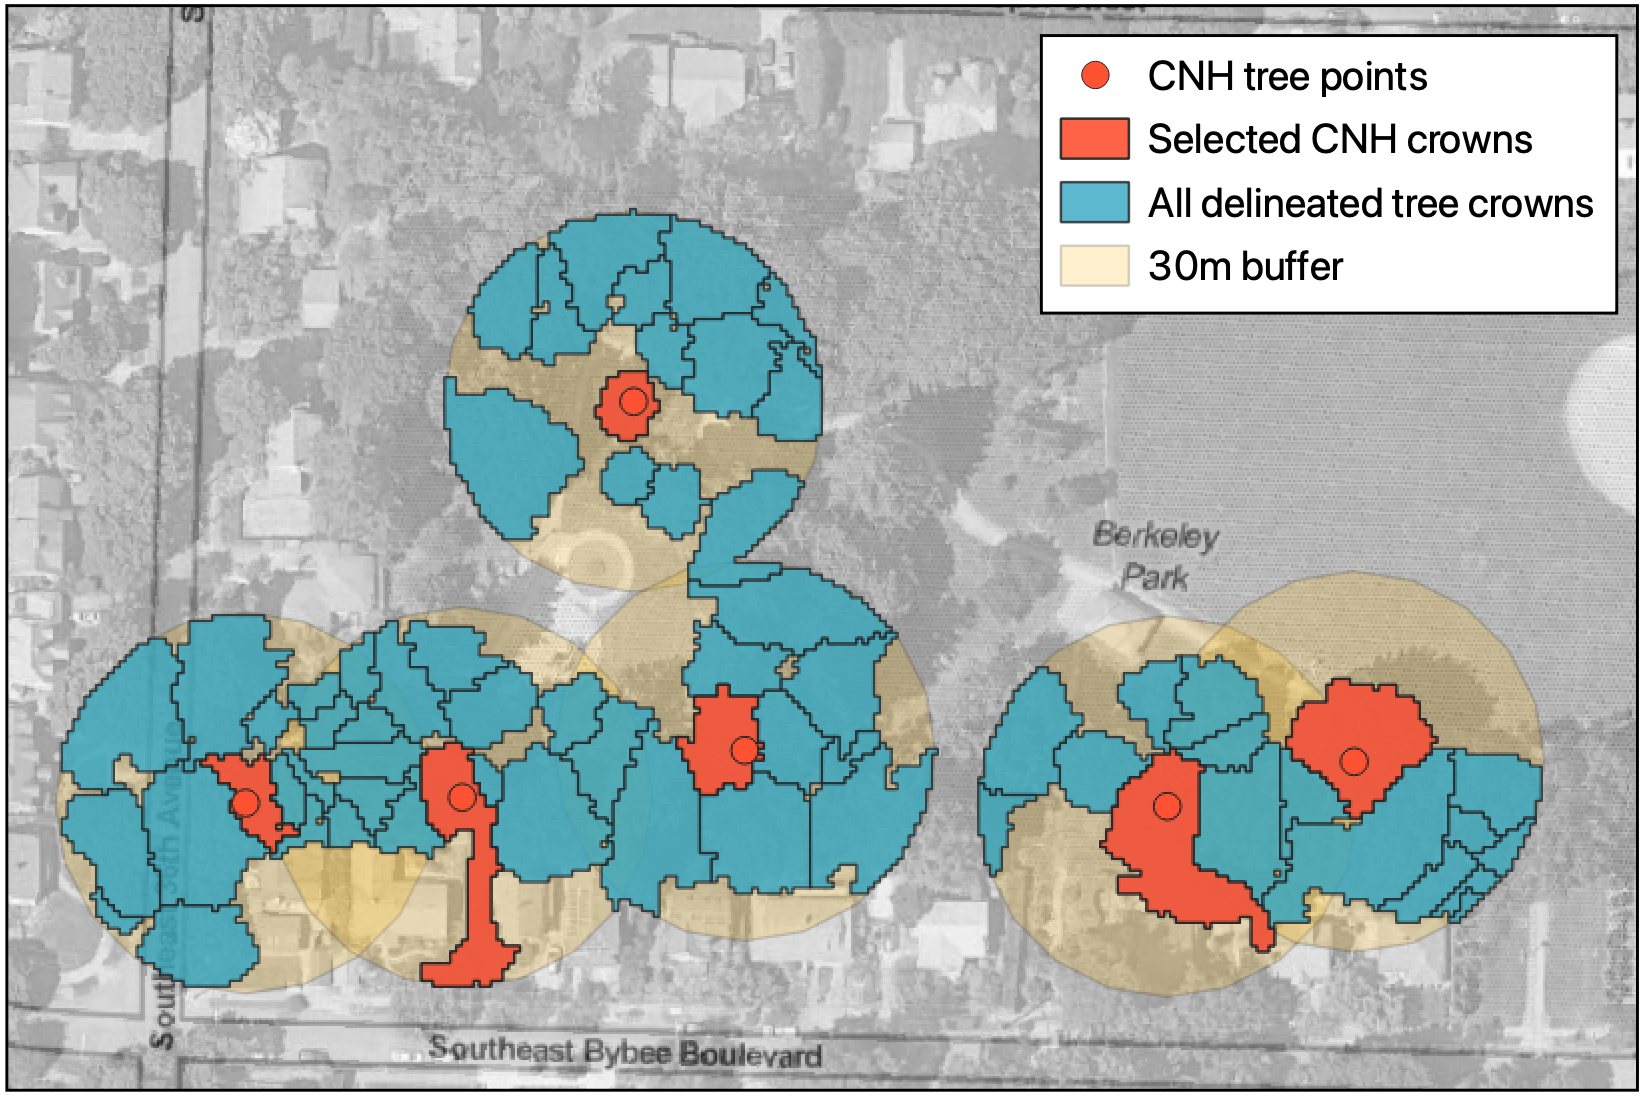
\includegraphics[width=0.8\linewidth]{figure/selected_lidar} 

}

\caption{LiDAR tree crown delineations with selected CNH crowns}\label{fig:unnamed-chunk-5}
\end{figure}
These three processes were repeated for random samples of 100 park trees and 100 street trees, though due to restrictions in file size for LiDAR processing, the sampling had to be constrained to an area of East Portland (Figure \ref{fig:clip-extent}). This extent was chosen to align with the sampling region of the CNH data, though it had to be shrunk slightly.
\begin{figure}

{\centering 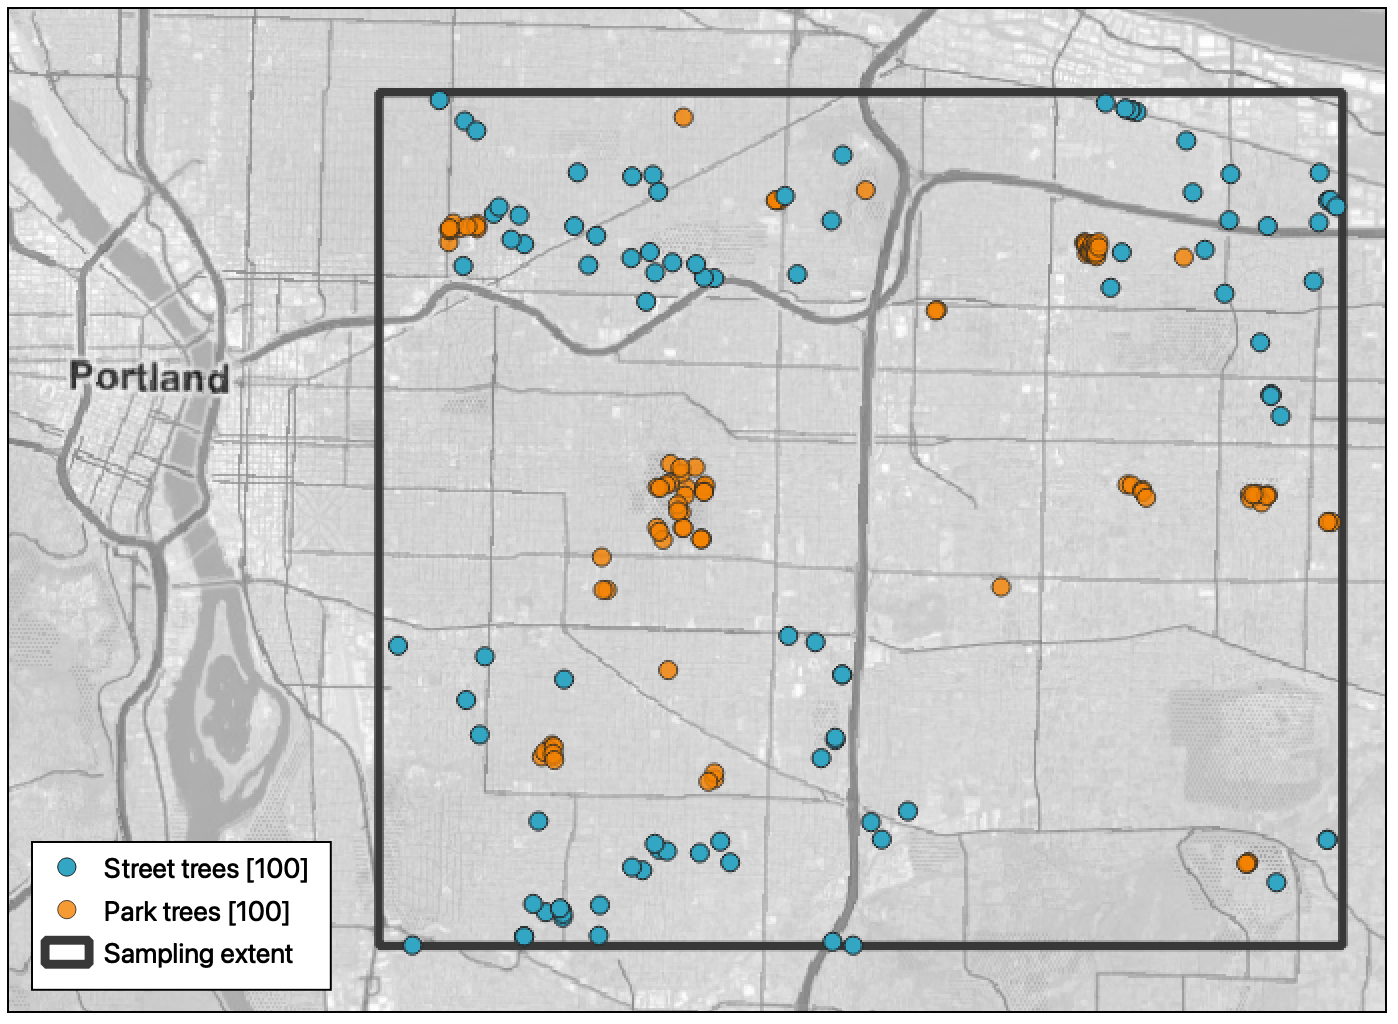
\includegraphics[width=0.8\linewidth]{figure/extent_and_samples} 

}

\caption{Geographic extent and random sampling}\label{fig:clip-extent}
\end{figure}
\begin{figure}

{\centering 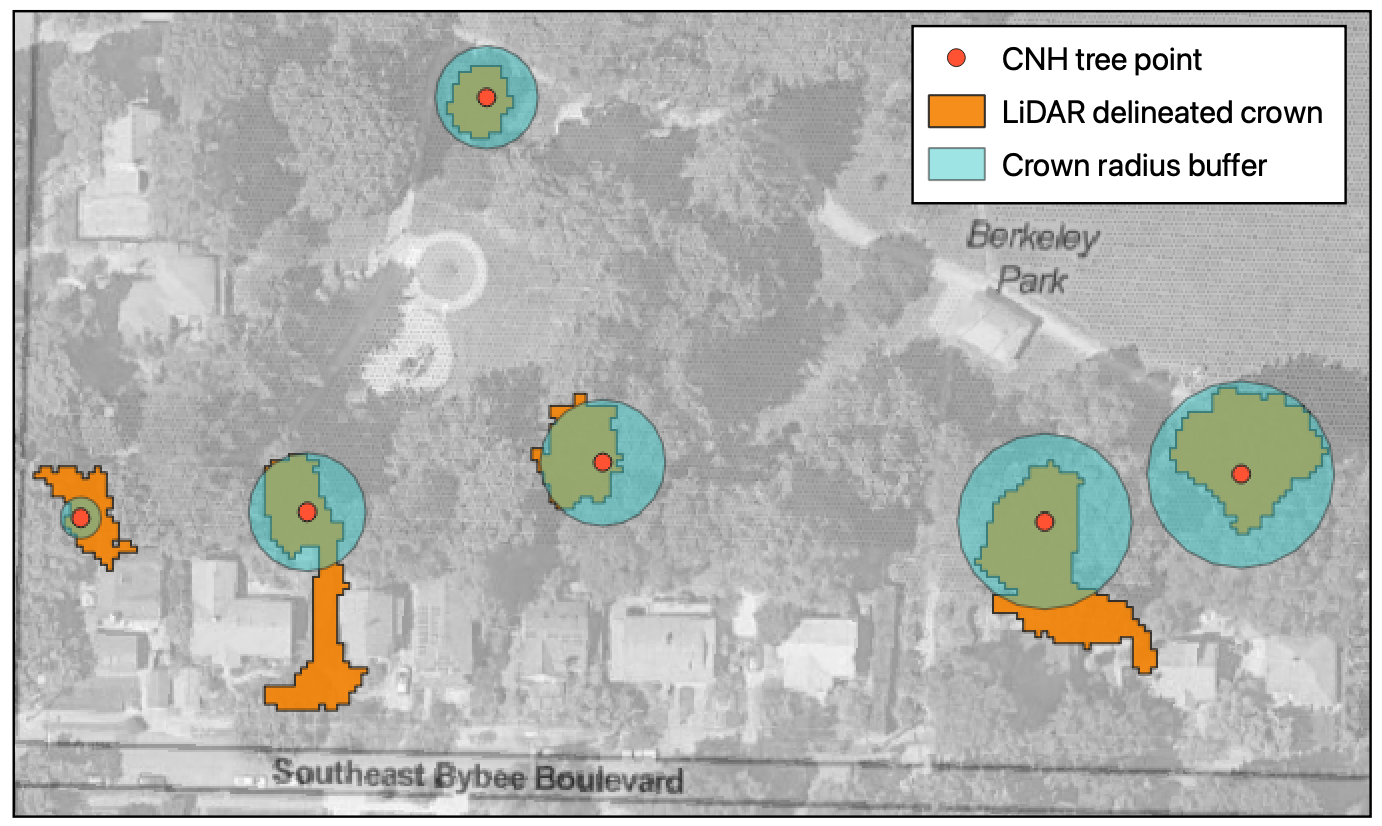
\includegraphics[width=0.8\linewidth]{figure/layered_outputs} 

}

\caption{LiDAR tree crown delineations with selected CNH crowns}\label{fig:unnamed-chunk-6}
\end{figure}
\hypertarget{modeling-tree-health}{%
\section{Modeling Tree Health}\label{modeling-tree-health}}

To tie all of my smaller pieces of data analysis together, I created a model to predict tree health categorization from NDVI values. I chose an ordinal logistic regression, which is used to model and predict the relationship between an ordinal categorical response variable and one or more explanatory variables, which can be either categorical or continuous. In order to use this type of model, I tested each model for the Proportional Odds Assumption, and

I used the CNH data as both my training and testing data. I chose to do this because of the limited sample size of CNH trees, and the uneven size of the health category ratings. Because of this, it is important to note that the model tests are an idealized version of a true model.

For each model, I created a confusion matrix to examine the validity of the model. A confusion matrix is a calculated cross-tabulation of observed and predicted classes, which in this case is health categorization, along with associated statistics. The two main statistics I use in my data analysis are overall accuracy and an un-weighted Kappa statistic. ``Accuracy'' refers to the sensitivity {[}\(\textrm{Sensitivity}= \frac{\textrm{True positive}}{\textrm{True positive + False negative}}\){]} and specificity {[}\(\textrm{Specificity}= \frac{\textrm{True negative}}{\textrm{True negative + False positive}}\){]} of the prediction.

\[
\textrm{Accuracy}= \frac{\textrm{Sensitivity + Specificity}}{2}
\]

Kappa (\(\kappa\)) refers to Cohen's Kappa Statistic which is used to measure inter and intra-rater reliability for categorical items.

\[
\kappa = \frac{p_o - p_e}{1 - p_e} = \frac{1 - p_o}{1 - p_e}
\]
where \(p_o\) is the relative observed agreement between the reference and prediction, and \(p_e\) is the hypothetical probability of agreement by chance. If the two raters (in this case the reference and prediction categorizations) are in complete agreement, then kappa = 1.

\hypertarget{results}{%
\chapter{Results}\label{results}}

\hypertarget{canopy-width-and-tree-height-model-1}{%
\section{Canopy Width and Tree Height Model}\label{canopy-width-and-tree-height-model-1}}

I used a third order polynomial regression to predict both tree height and crown width from tree DBH. In order to account for expected differences between species, I included species as an interaction term. I chose a third order polynomial because it not only encapsulated the relationship between DBH and tree height as well as DBH and canopy width, but it also was the most accurate when modeling the individual species. While the
The tree height model has an adjusted R-squared value of 0.78, and a P-value of \textless{} 2.2e-16 (Figure \ref{fig:height-model}). The crown width model has an adjusted R-squared value of 0.72, and a P-value of \textless{} 2.2e-16 (Figure \ref{fig:width-model-g}, \ref{tree-model-eqs}).
\begin{figure}
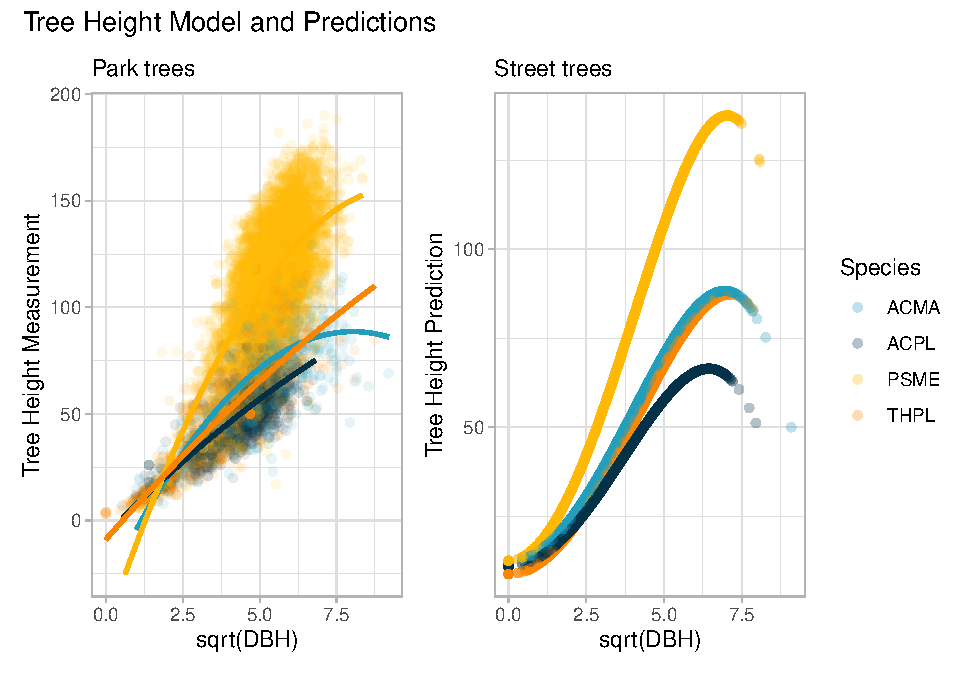
\includegraphics[width=0.8\linewidth]{thesis_files/figure-latex/height-model-1} \caption[Tree height predictive model]{Predictive model for tree height from measured DBH. A third order polynomial regression was used in order to account for the variation between species. (Adjusted R-squared = 0.72, P <2.2e-16)}\label{fig:height-model}
\end{figure}
\begin{figure}
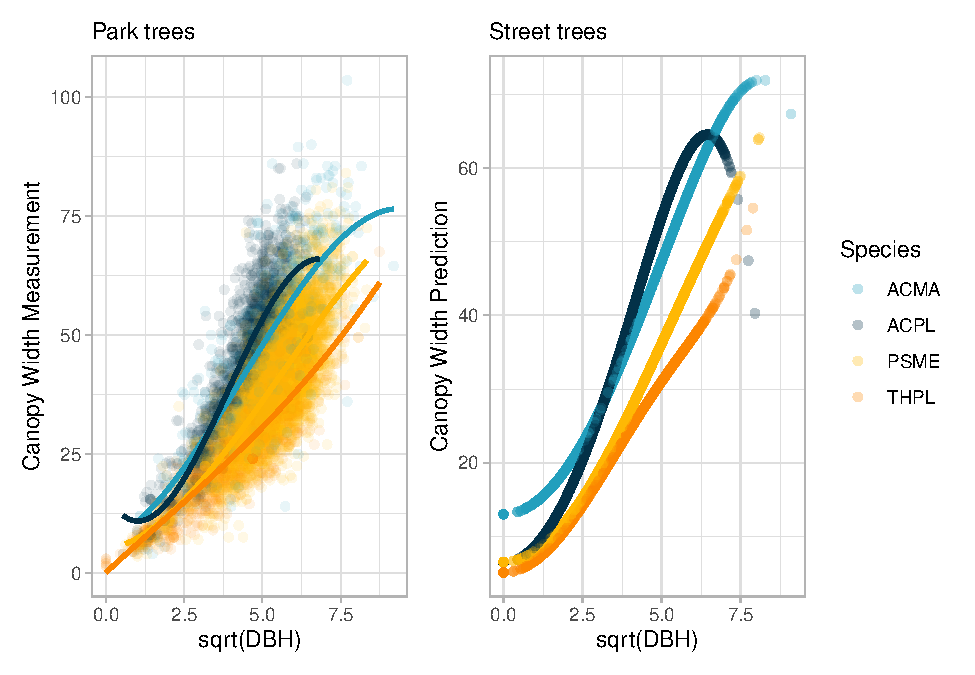
\includegraphics[width=0.8\linewidth]{thesis_files/figure-latex/width-model-g-1} \caption[Crown width predictive model]{Third order polynomial model for predicting tree crown width based on measured DBH and species, with predictions for street trees. (R-squared = 0.72,  P <2.2e-16)}\label{fig:width-model-g}
\end{figure}
\hypertarget{point-method-1}{%
\section{Point Method}\label{point-method-1}}

With the selection of CNH trees and 2021 NDVI data, a statistical analysis of the point value method shows that there is a statistically significant difference in the average NDVI values between health categorizations of ``Fair'' and ``Good'' (ANOVA, \(F_{2, 109} = 3.892\), \(P = 0.023\), TukeyHSD). There is a general positive correlation between NDVI and health category, specifically Fair and Good. The relationship between health and NDVI is more apparent in the two maple species, but still holds in the ``fair'' and ``good'' categories in the two coniferous species (Figure \ref{fig:point-species}).
\begin{figure}
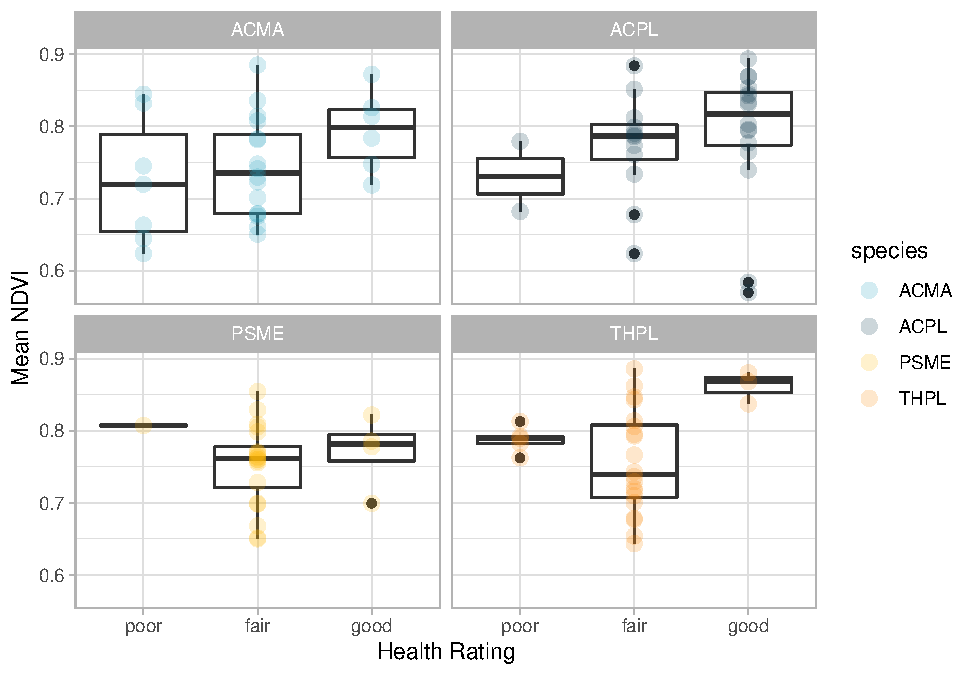
\includegraphics[width=1\linewidth]{thesis_files/figure-latex/point-species-1} \caption[Point Method NDVI and Health Rating, by Species]{NDVI extracted for CNH trees using the point method compared to CNH tree health categorization. There is a statistically significant difference between Fair and Good (ANOVA, $F_{2, 109} = 3.892$, $P = 0.023$, TukeyHSD)}\label{fig:point-species}
\end{figure}
\hypertarget{radius-method-1}{%
\section{Radius Method}\label{radius-method-1}}

With the radius method of pixel selection and crown delineation, there is a statistically significant difference in the mean NDVI values for health categories (ANOVA, \(F_{2,109}=4.923\), \(P = 0.0089\); TukeyHSD: good-poor \(P = 0.033\), good-fair \(P = 0.014\)). Similar to the point method, there is a larger difference in average NDVI between the ``fair'' and ``good'' categories than ``poor'' and ``fair'', and with the radius method, this is now a statistically significant difference (Figure \ref{fig:radius-species}).
\begin{figure}
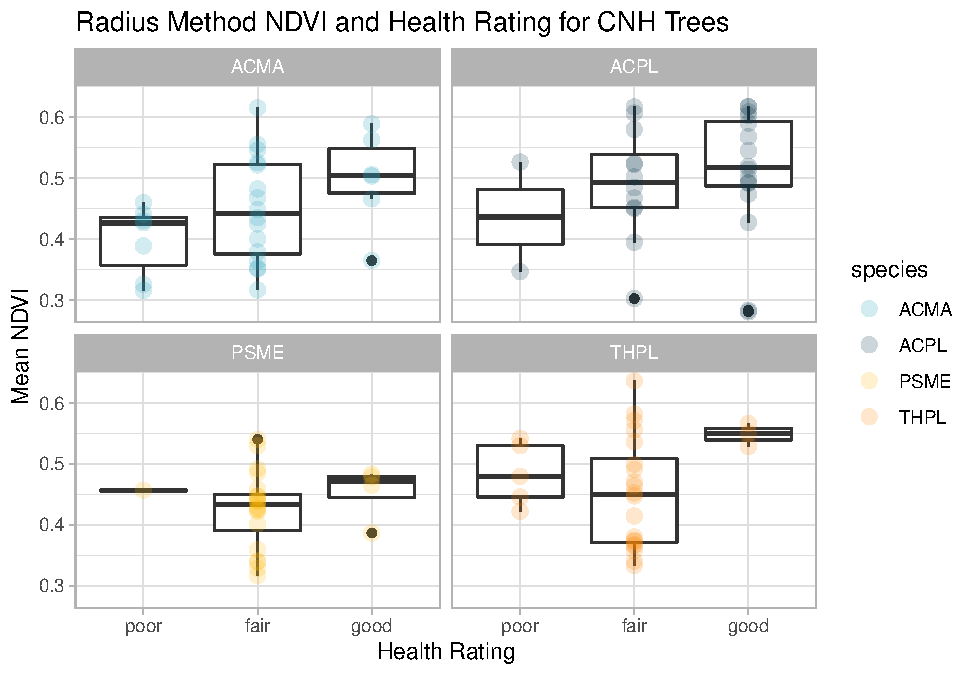
\includegraphics[width=1\linewidth]{thesis_files/figure-latex/radius-species-1} \caption[Radius method mean NDVI and health condition by species]{Boxplot of average NDVI from radius method and health condition, by species. The relationship berween NDVI and health category is strongest in the maples, but still somewhat aparent in the conifers. (ANOVA, $F_{2,109}=4.923$, $P = 0.0089$; TukeyHSD: good-poor $P = 0.033$, good-fair $P = 0.014$)}\label{fig:radius-species}
\end{figure}
\hypertarget{lidar-method-1}{%
\section{LiDAR Method}\label{lidar-method-1}}

There is a statistically significant difference in NDVI between health categories for the LiDAR method, specifically between good and fair (ANOVA, \(F_{2,101} = 5.405\), \(P = 0.00589\), TukeyHSD). The same relationship between NDVI and health condition for the maples that was seen in the point and radius method is seen here (Figure \ref{fig:lidar-species}).
\begin{figure}
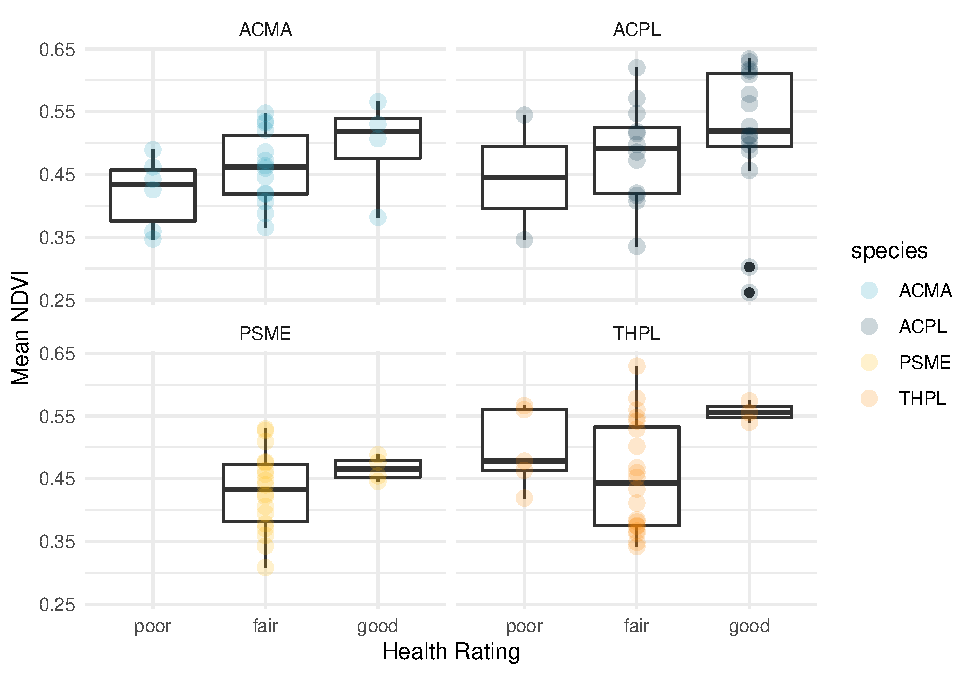
\includegraphics[width=1\linewidth]{thesis_files/figure-latex/lidar-species-1} \caption[NDVI and health condition for LiDAR method]{Boxplot of average NDVI from LiDAR method and health condition for each species. Due to the nature of the LiDAR delineation algorithm, no crown was detected for the PSME individual with a poor health rating. The difference between good and fair average NDVIs is statistically significant (ANOVA, $F_{2,101} = 5.405$, $P = 0.00589$, TukeyHSD)}\label{fig:lidar-species}
\end{figure}
Another aspect of the LiDAR delineation method is the potential for data loss. Five ACMA and three PSME individuals were lost in the LiDAR crown delineation process. If this was with a very large sample size the data loss would likely not be detrimental but especially with a sample size such as mine, a loss of eight trees is a loss of 5\% of the total data, 17\% loss for ACMA, and 12\% loss for THPL.

\hypertarget{method-comparison}{%
\section{Method Comparison}\label{method-comparison}}

There is a statistically significant difference in NDVI values for the three different pixel selection methods (ANOVA, \(F_{2, 325}=517.8\), \(P < 2e-16\); TukeyHSD, radius-point \(P = 0.00\), lidar-point \(P = 0.00\)). When the species are clumped, the three methods show very similar patterns, though the NDVI values are higher for the point method than either of the other two methods (Figure \ref{fig:methods-all-species}). When all three methods are compared along with species, we can see that the general trend of health rating and NDVI is consistent within each species, but varies across methods (Figure \ref{fig:methods-species}). Additionally, the pattern between health rating and NDVI is also very similar between trees of the same functional type. Because of the similarities in health patter, I included additional testing examining the difference in species specificity addition versus functional type separation.
\begin{figure}
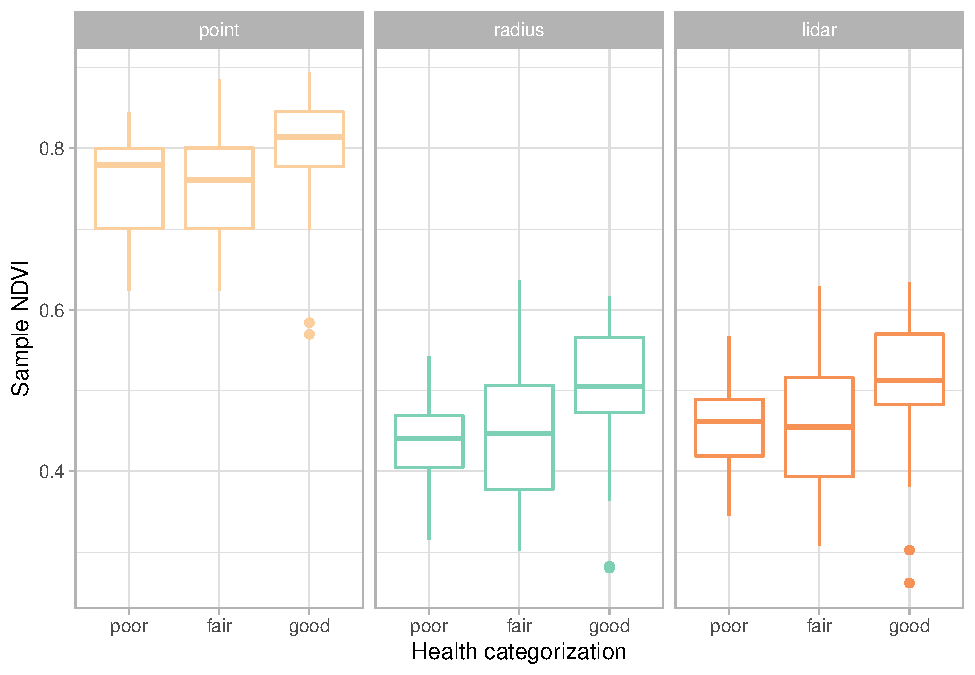
\includegraphics[width=0.8\linewidth]{thesis_files/figure-latex/methods-all-species-1} \caption[NDVI and health rating comparison across methods]{Average NDVI values from all three pixel selection methods with CNH health rating. There is a statistically significant difference in mean NDVI between point and both radius and lidar methods. (ANOVA, $F_{2, 325}=517.8$, $P = <2e-16$, TukeyHSD: radius-point $P = 0.00$, lidar-point $P = 0.00$)}\label{fig:methods-all-species}
\end{figure}
\begin{figure}
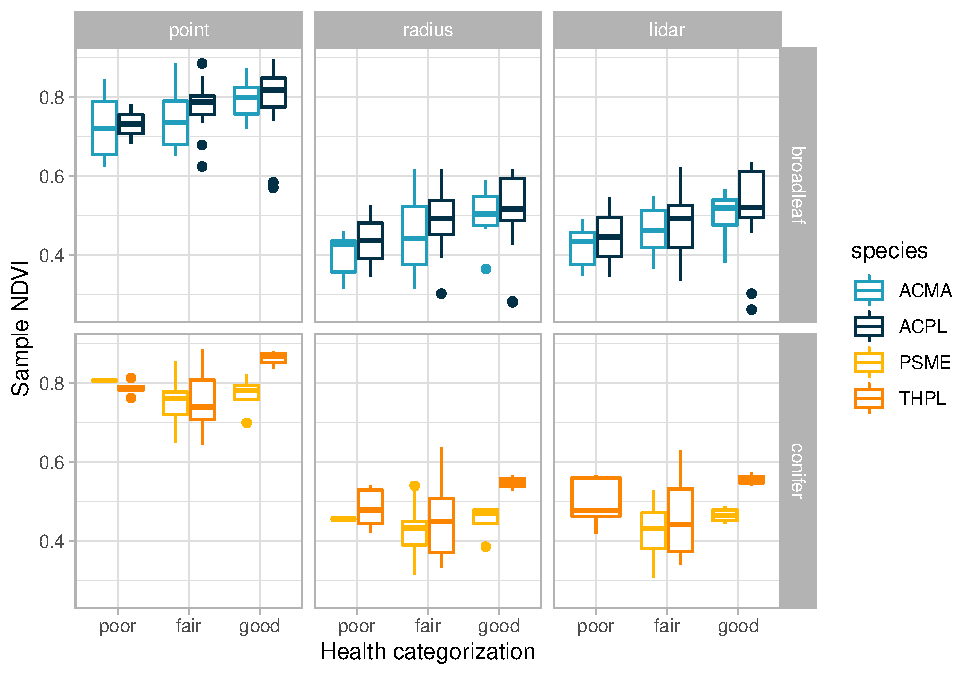
\includegraphics{thesis_files/figure-latex/methods-species-1} \caption[Average NDVI comparison between species and methods.]{Average NDVI for each health category, split by tree species and pixel selection method. The general trends remain the same within species, but vary among pixel selection methods.}\label{fig:methods-species}
\end{figure}
Another important factor to consider when comparing the three pixel selection methods is the amount of pixels used in the NDVI analysis. For the point method, each NDVI value is based off one singular point.
\begin{Shaded}
\begin{Highlighting}[]
\NormalTok{radius\_sample\_data }\OtherTok{\textless{}{-}} \FunctionTok{read\_csv}\NormalTok{(}\StringTok{"data/radius\_sample\_data.csv"}\NormalTok{) }\SpecialCharTok{\%\textgreater{}\%}
\NormalTok{    dplyr}\SpecialCharTok{::}\FunctionTok{select}\NormalTok{(}\SpecialCharTok{{-}}\DecValTok{4}\NormalTok{, }\SpecialCharTok{{-}}\DecValTok{5}\NormalTok{) }\SpecialCharTok{\%\textgreater{}\%}
    \FunctionTok{mutate}\NormalTok{(}\AttributeTok{method =} \StringTok{"radius"}\NormalTok{)}
\NormalTok{lidar\_sample\_data }\OtherTok{\textless{}{-}} \FunctionTok{read\_csv}\NormalTok{(}\StringTok{"data/lidar\_sample\_data.csv"}\NormalTok{) }\SpecialCharTok{\%\textgreater{}\%}
\NormalTok{    dplyr}\SpecialCharTok{::}\FunctionTok{select}\NormalTok{(}\SpecialCharTok{{-}}\DecValTok{4}\NormalTok{) }\SpecialCharTok{\%\textgreater{}\%}
    \FunctionTok{mutate}\NormalTok{(}\AttributeTok{method =} \StringTok{"LiDAR"}\NormalTok{)}
\NormalTok{count\_sample\_data }\OtherTok{\textless{}{-}}\NormalTok{ lidar\_sample\_data }\SpecialCharTok{\%\textgreater{}\%}
    \FunctionTok{bind\_rows}\NormalTok{(radius\_sample\_data)}
\FunctionTok{ggplot}\NormalTok{(}\AttributeTok{data =}\NormalTok{ count\_sample\_data, }\FunctionTok{aes}\NormalTok{(}\AttributeTok{x =}\NormalTok{ method, }\AttributeTok{y =}\NormalTok{ ndvi\_count,}
    \AttributeTok{color =}\NormalTok{ species)) }\SpecialCharTok{+} \FunctionTok{geom\_boxplot}\NormalTok{(}\AttributeTok{outlier.shape =} \ConstantTok{NA}\NormalTok{) }\SpecialCharTok{+} \FunctionTok{geom\_point}\NormalTok{(}\AttributeTok{position =} \FunctionTok{position\_jitterdodge}\NormalTok{(}\AttributeTok{jitter.width =} \FloatTok{0.1}\NormalTok{),}
    \AttributeTok{alpha =} \FloatTok{0.3}\NormalTok{) }\SpecialCharTok{+} \FunctionTok{scale\_color\_manual}\NormalTok{(}\AttributeTok{values =}\NormalTok{ species\_pal) }\SpecialCharTok{+}
    \FunctionTok{labs}\NormalTok{(}\AttributeTok{x =} \StringTok{"Pixel selection method"}\NormalTok{, }\AttributeTok{y =} \StringTok{"Pixel count"}\NormalTok{, }\AttributeTok{color =} \StringTok{"Tree species"}\NormalTok{)}
\end{Highlighting}
\end{Shaded}
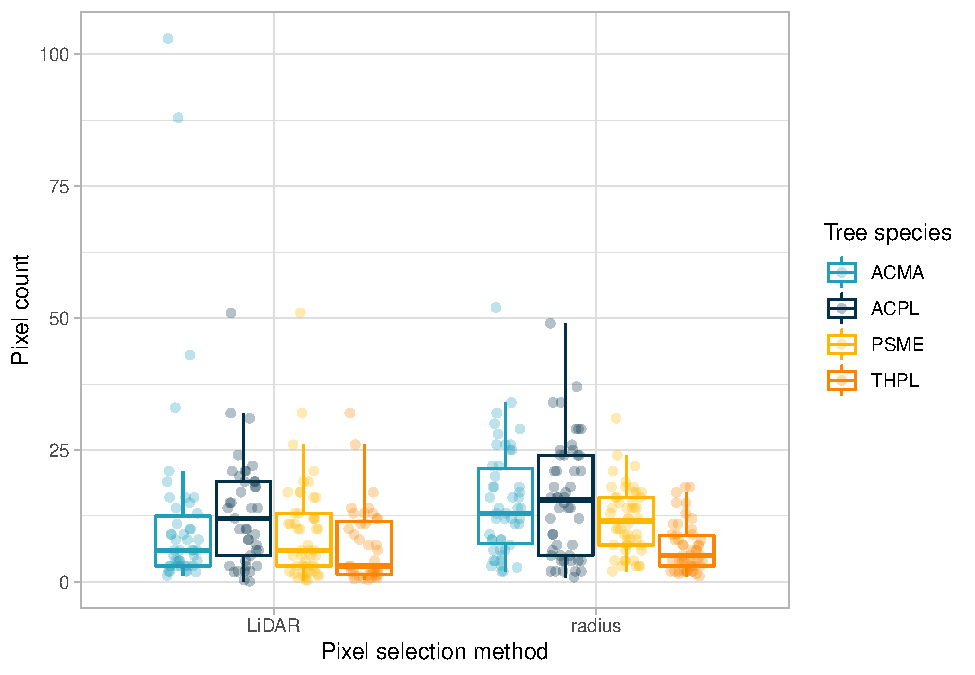
\includegraphics{thesis_files/figure-latex/unnamed-chunk-15-1.pdf}
\begin{Shaded}
\begin{Highlighting}[]
\FunctionTok{ggplot}\NormalTok{(}\AttributeTok{data =}\NormalTok{ count\_sample\_data, }\FunctionTok{aes}\NormalTok{(}\AttributeTok{x =}\NormalTok{ ndvi\_mean, }\AttributeTok{y =}\NormalTok{ ndvi\_count,}
    \AttributeTok{color =}\NormalTok{ species)) }\SpecialCharTok{+} \FunctionTok{geom\_point}\NormalTok{() }\SpecialCharTok{+} \FunctionTok{scale\_color\_manual}\NormalTok{(}\AttributeTok{values =}\NormalTok{ species\_pal) }\SpecialCharTok{+}
    \FunctionTok{labs}\NormalTok{(}\AttributeTok{x =} \StringTok{"Average NDVI"}\NormalTok{, }\AttributeTok{y =} \StringTok{"Pixel count"}\NormalTok{, }\AttributeTok{color =} \StringTok{"Tree species"}\NormalTok{)}
\end{Highlighting}
\end{Shaded}
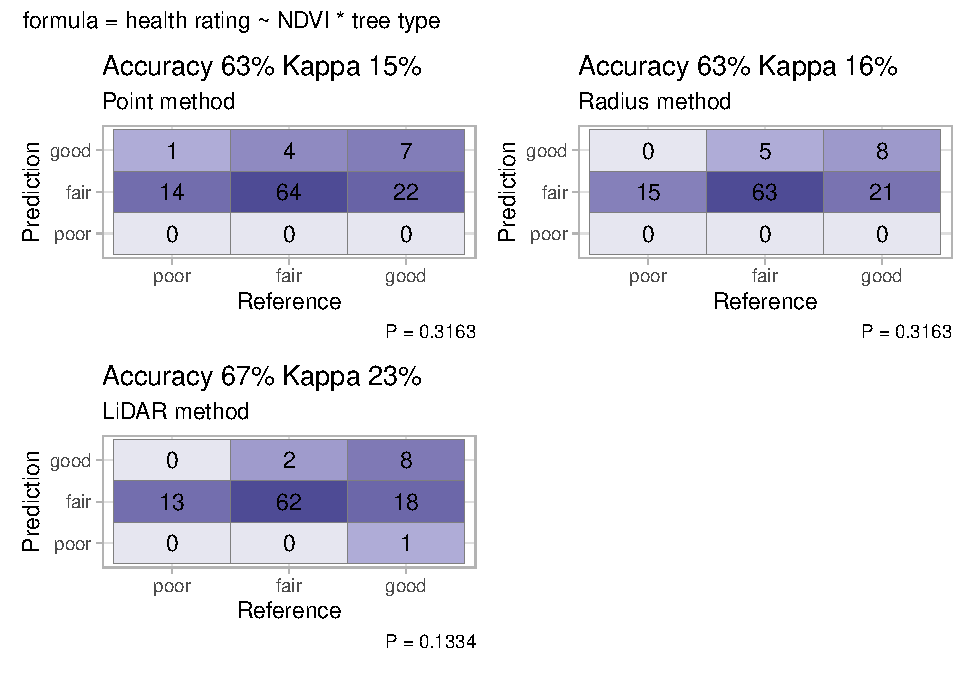
\includegraphics{thesis_files/figure-latex/unnamed-chunk-15-2.pdf}

\hypertarget{predictive-model}{%
\section{Predictive Model}\label{predictive-model}}

In order to determine the impact of differentiating by species in predictive models, I ran three different models for each point selection method, moving from least to most specific: a model that only uses NDVI to predict health rating, a model that includes functional tree type as an interaction term, and a third model that includes species as an interaction term. Due to the limited sample size of the data I am working with, the following models are trained and tested on the same data. If it were to work perfectly, the model would correctly predict the health condition of a CNH tree 100\% of the time. The data I use is not perfect, and the models are not perfect either. However, they are likely an idealized version of how model testing and training would work in reality.
With the point method data, the first model with no interaction term led to all tree points being rated as ``Fair''. The addition of tree type as an interaction term led to an increase in predictions of ``good'' health trees, and increased kappa from 0\% to 15\%. The overall accuracy only increased by 2\%, but kappa is more informative in terms of model validity than the accuracy score. Using tree species instead of tree type further improved the kappa of the model. The number of ``good'' trees that were correctly predicted increased from 7 to 13, but additionally the number of ``fair'' trees that were correctly predicted dropped from 64 to 59, with the new predictions as ``good''. (Figure \ref{point-model-split}). None of these models with the point method were able to correctly predict any trees with poor health categorization.

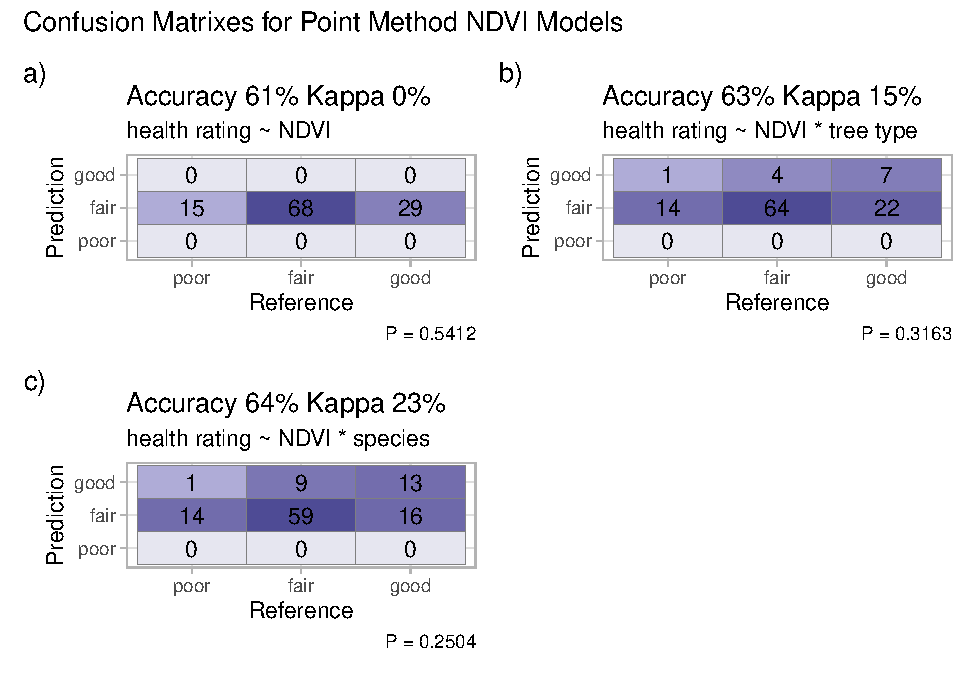
\includegraphics[width=0.9\linewidth]{thesis_files/figure-latex/point-model-split-1}

The radius method was slightly more successful than the point method for the model, with all three method models performing better than those for the point method. From just NDVI to NDVI * tree type, there was an increase in 9 trees to good ratings. Including no species or tree type specification in the predictive model still seems to perform the worst of the three models. The main takeaway from the radius method models is that with the inclusion of species as an interaction term with the radius data, we see our first predictions of the ``poor'' category. The radius method does involve more pixels than the point method, and with the range in NDVI values being lower than that of the point method it makes sense that there is an increase in ``poor'' rated trees. However, out of the 15 reference trees with health ratings of ``poor'', only one was correctly predicted as such (Figure \ref{fig:radius-model-split}).
\begin{figure}
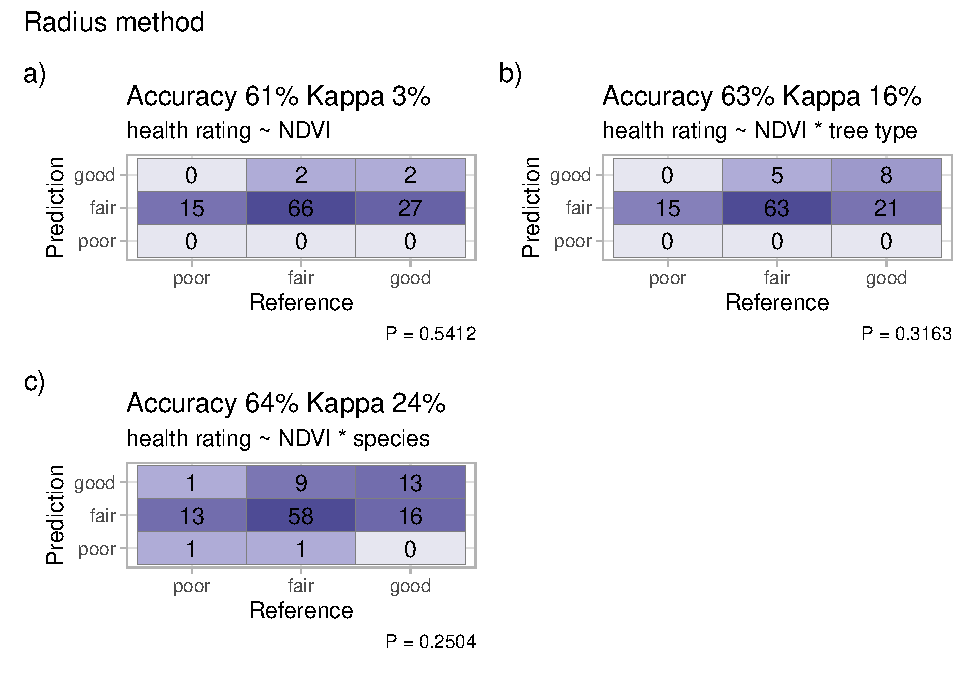
\includegraphics{thesis_files/figure-latex/radius-model-split-1} \caption[Confusion matrixes for Radius data model]{Confusion matrixes for each species predictions with radius method data}\label{fig:radius-model-split}
\end{figure}
The LiDAR data was the most effective out of the three methods at predicting tree health, but also had the only occurance of a ``good'' tree being predicted as ``poor''.

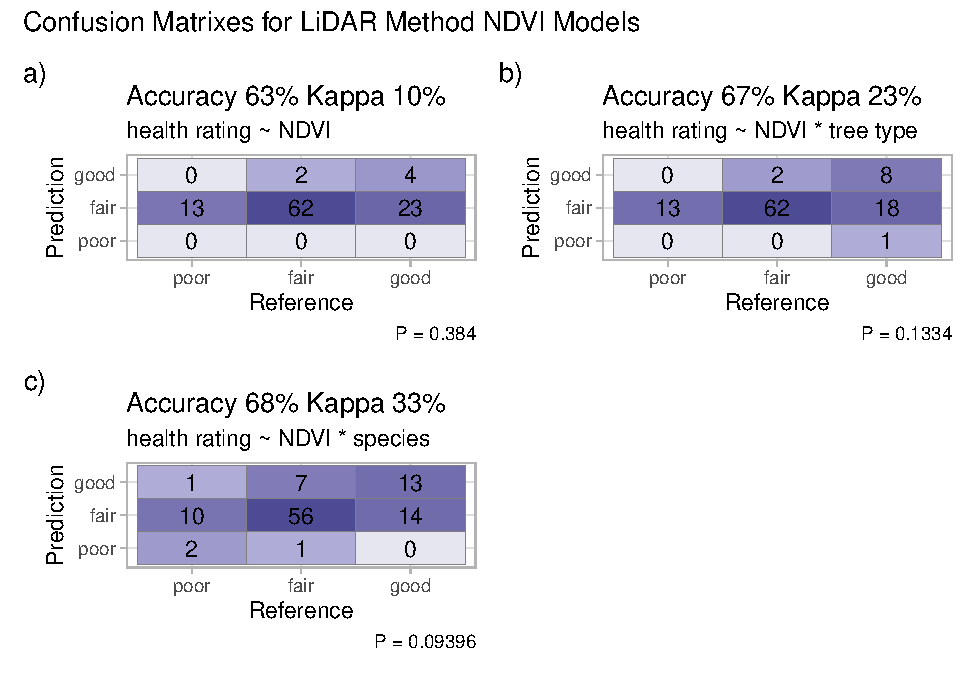
\includegraphics{thesis_files/figure-latex/lidar-model-split-1.pdf}

A predictive model was also run with all species together, but with species as an interaction term in the formula. This showed better results than when the species were split, but it seems that most of that is due to increased overall sample size.

Due to the variation in sample sizes for each health condition category, I sampled down the data so each health category had the same number of points. This improved the results of the model by a lot.

Given the uneven number of data points available for the varying health conditions, I down-sampled each health category to the smallest number of points in a given category (point = 15, radius = 15, LiDAR = 13). When the predictive models were ran with the even category sizes, the results were statistically significant for all three pixel selection models. For the poi

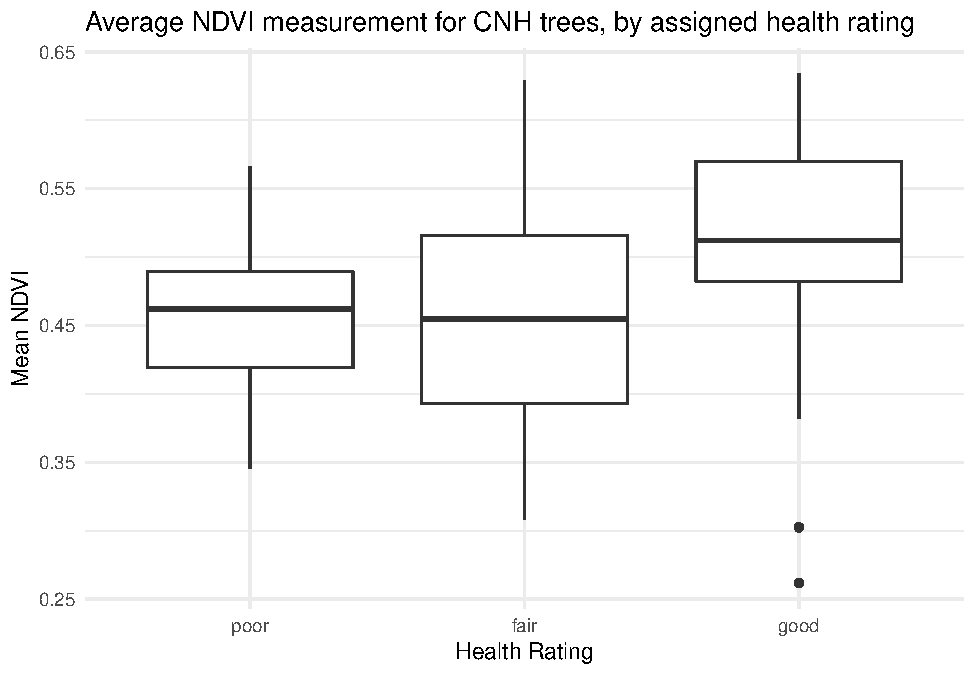
\includegraphics{thesis_files/figure-latex/unnamed-chunk-16-1.pdf}

\hypertarget{discussion}{%
\chapter{Discussion}\label{discussion}}

testing

\appendix

\hypertarget{data}{%
\chapter{Additional Data}\label{data}}

\hypertarget{tree-model-eqs}{%
\section{Tree Height and Crown Width Predictive Model Equations}\label{tree-model-eqs}}

\textbf{ACMA equations:} (\textit{x} = DBH)
\begin{equation}
\textrm{Tree Height} = 8.977 + 3.617x -0.049x^{2} + 0.001x^{3}  \\
\end{equation}
\begin{equation}
\textrm{Crown Width} = 13.01 + 1.593x - 0.007x^{2} + 0.0004x^{3} \\
\end{equation}
\textbf{ACPL equations:} (\textit{x} = DBH)
\begin{equation}
\textrm{Tree Height} = 10.955+ 2.67x -0.032x^2 + 0.001x^3  \\
\end{equation}
\begin{equation}
\textrm{Crown Width} = 6.445 + 2.29x - 0.009x^2 - 0.0002x^3 \\
\end{equation}
\textbf{PSME equations:} (\textit{x} = DBH)
\begin{equation}
\textrm{Tree Height} = -4.497 + 7.516x - 0.146x^2 + 0.001x^3 \\
\end{equation}
\begin{equation}
\textrm{Crown Width} = 6.536 + 1.471x - 0.013x^2 + 0.0005x^3 \\
\end{equation}
\textbf{THPL equations:} (\textit{x} = DBH)
\begin{equation}
\textrm{Tree Height} = 7.311 + 3.457x - 0.0473x^2 + 0.001x^3 \\
\end{equation}
\begin{equation}
\textrm{Crown Width} = 5.113 + 1.622x - 0.032x^2 + 0.0002x^3 \\
\end{equation}
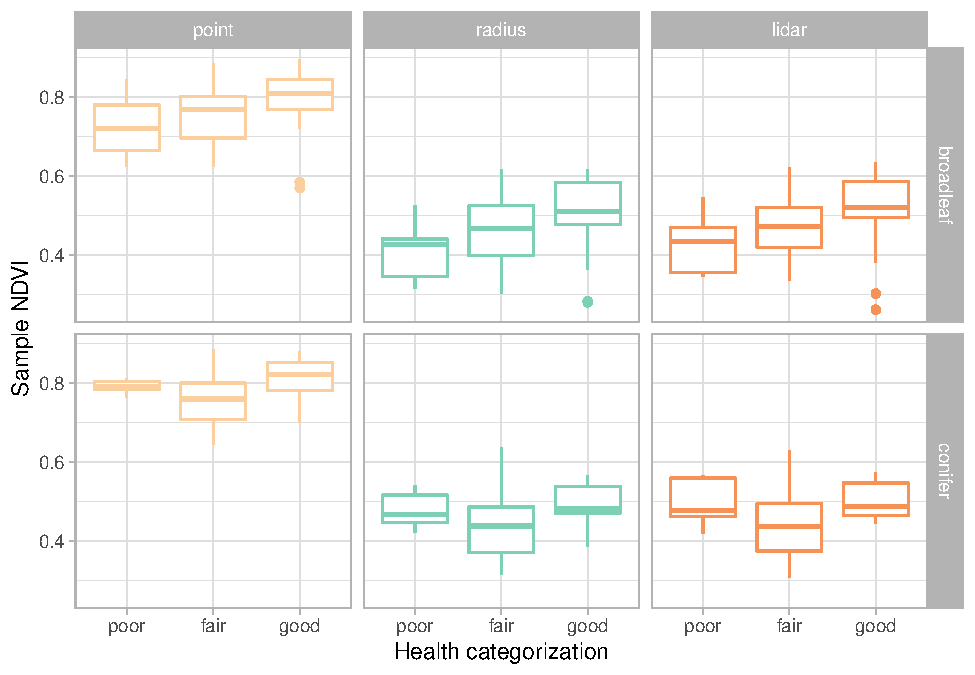
\includegraphics{thesis_files/figure-latex/extra-graph-1-1.pdf}

\hypertarget{extra-modeling-graphics}{%
\section*{extra modeling graphics}\label{extra-modeling-graphics}}
\addcontentsline{toc}{section}{extra modeling graphics}

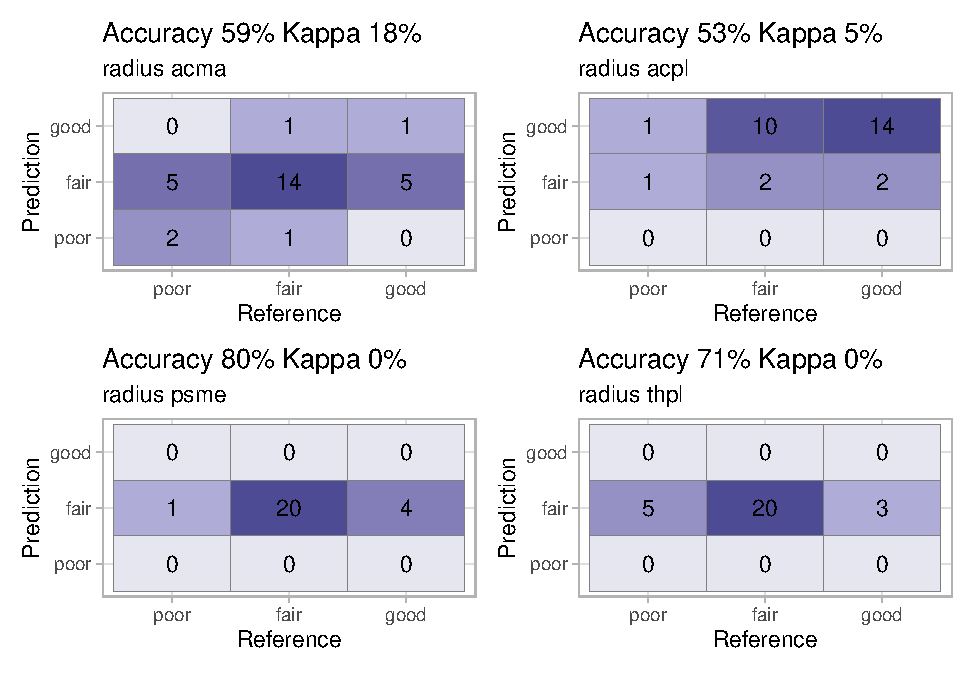
\includegraphics{thesis_files/figure-latex/unnamed-chunk-17-1.pdf} 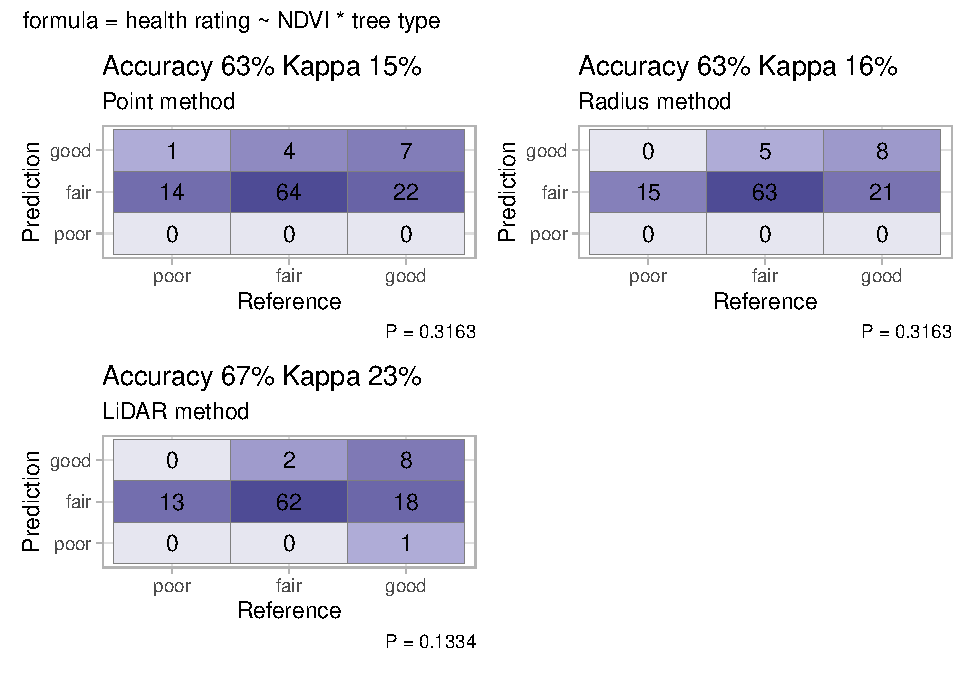
\includegraphics{thesis_files/figure-latex/unnamed-chunk-17-2.pdf} 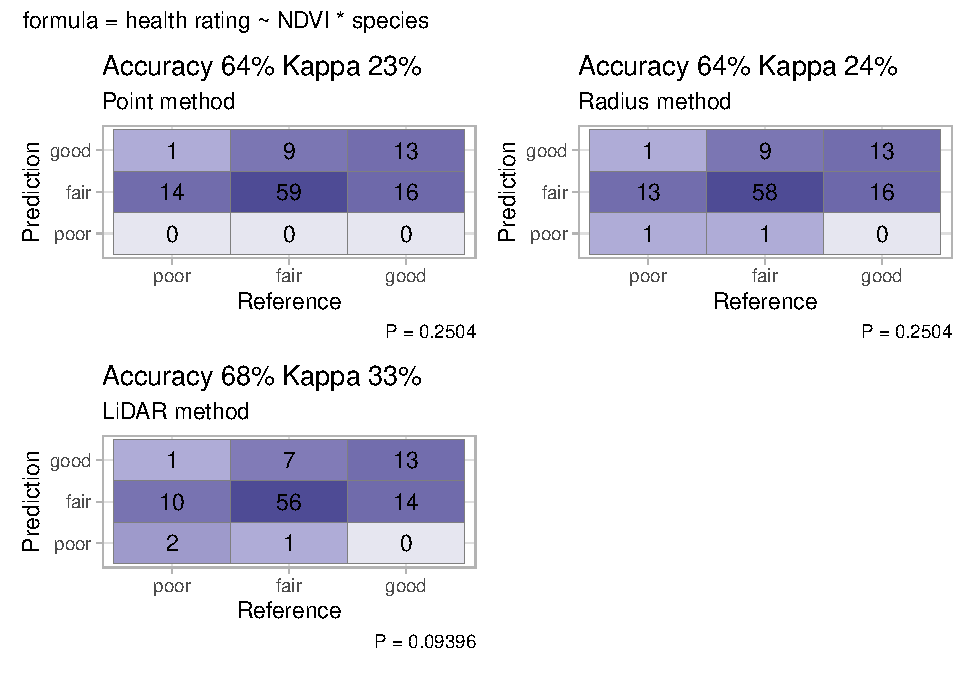
\includegraphics{thesis_files/figure-latex/unnamed-chunk-17-3.pdf}

\hypertarget{radius-and-lidar-model-tests}{%
\section*{Radius and LiDAR model tests}\label{radius-and-lidar-model-tests}}
\addcontentsline{toc}{section}{Radius and LiDAR model tests}

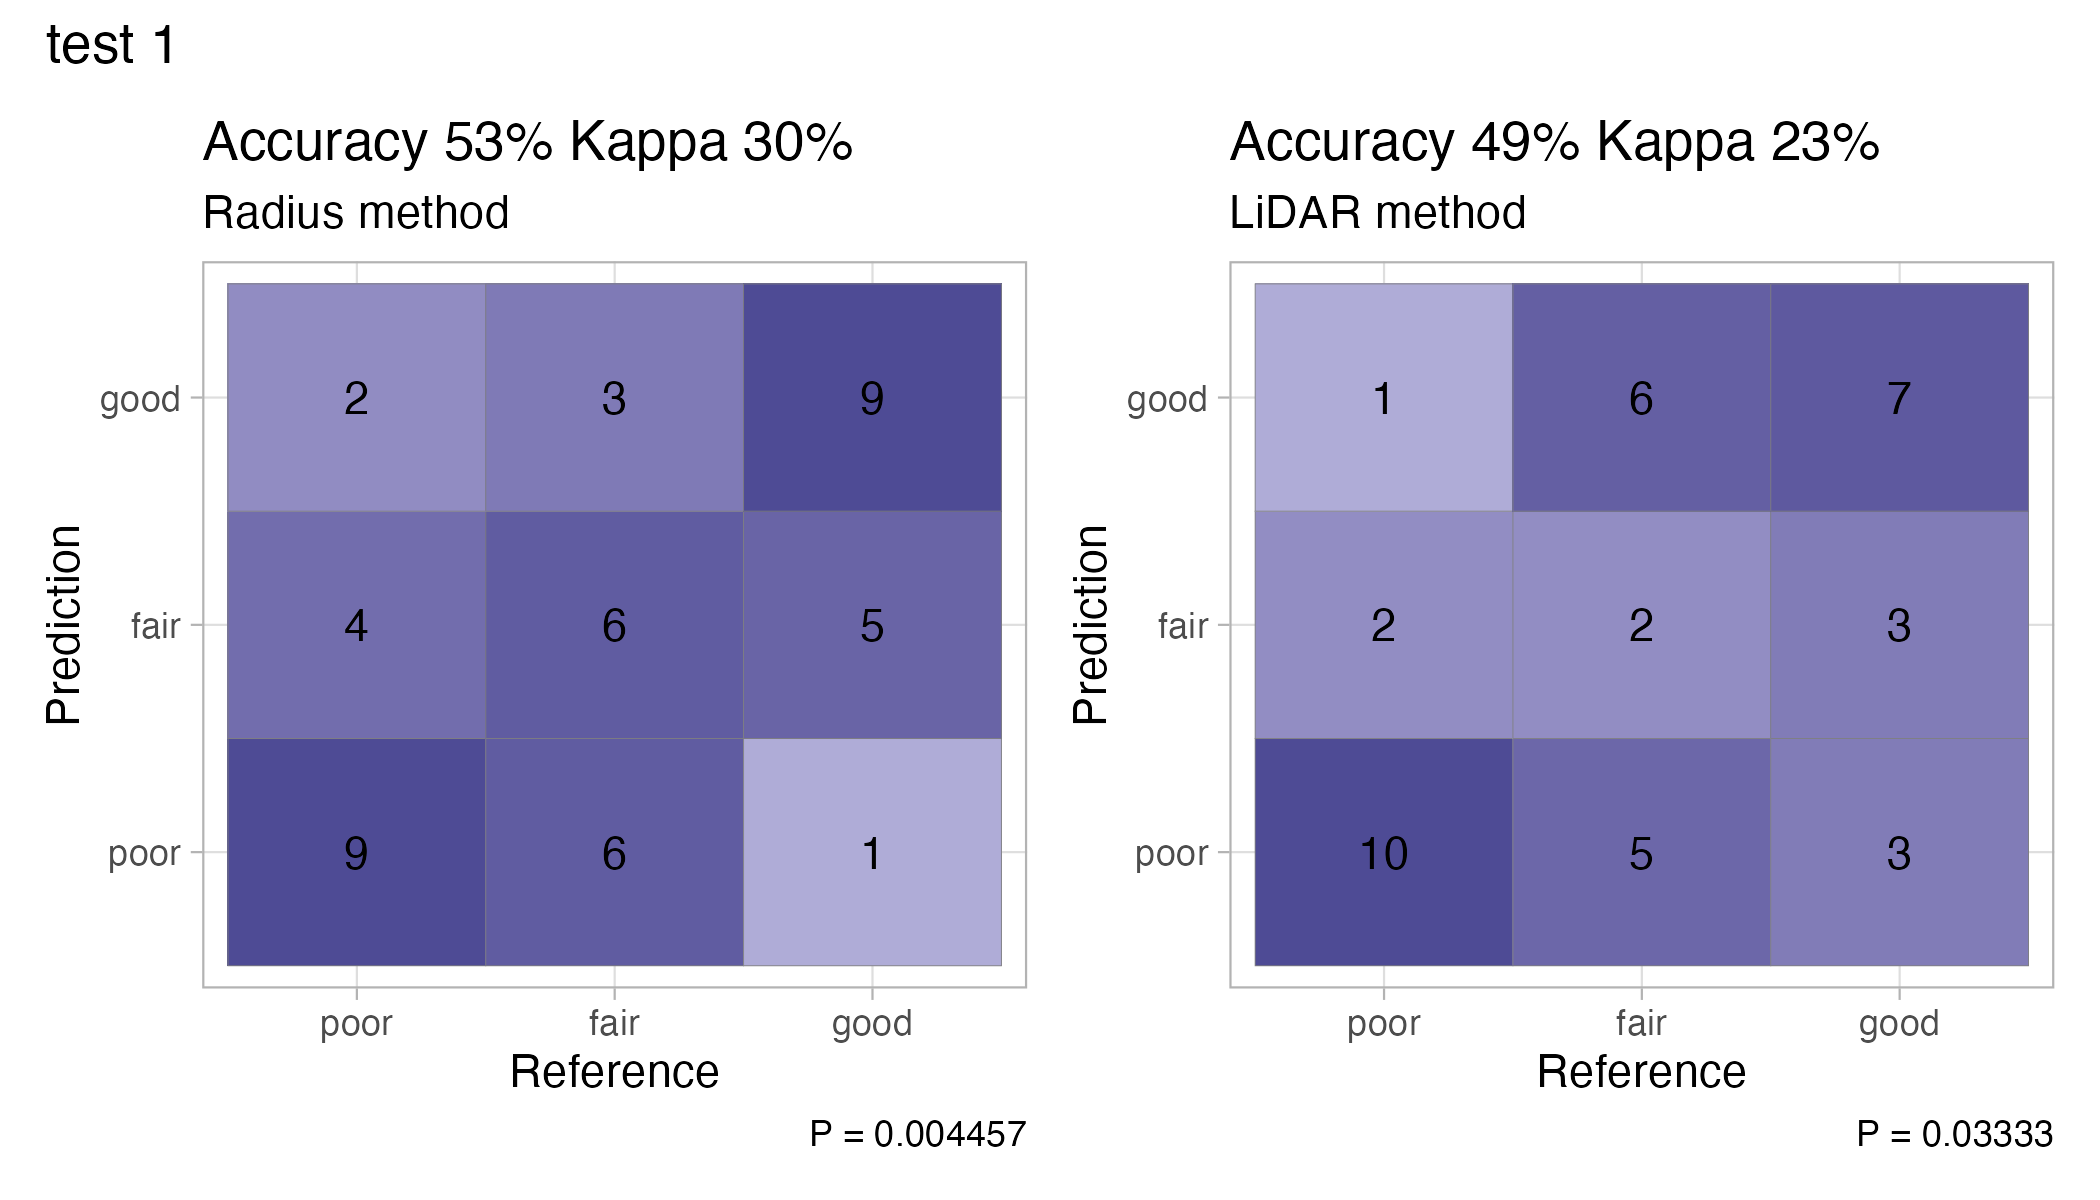
\includegraphics[width=0.85\linewidth]{figure/test1}
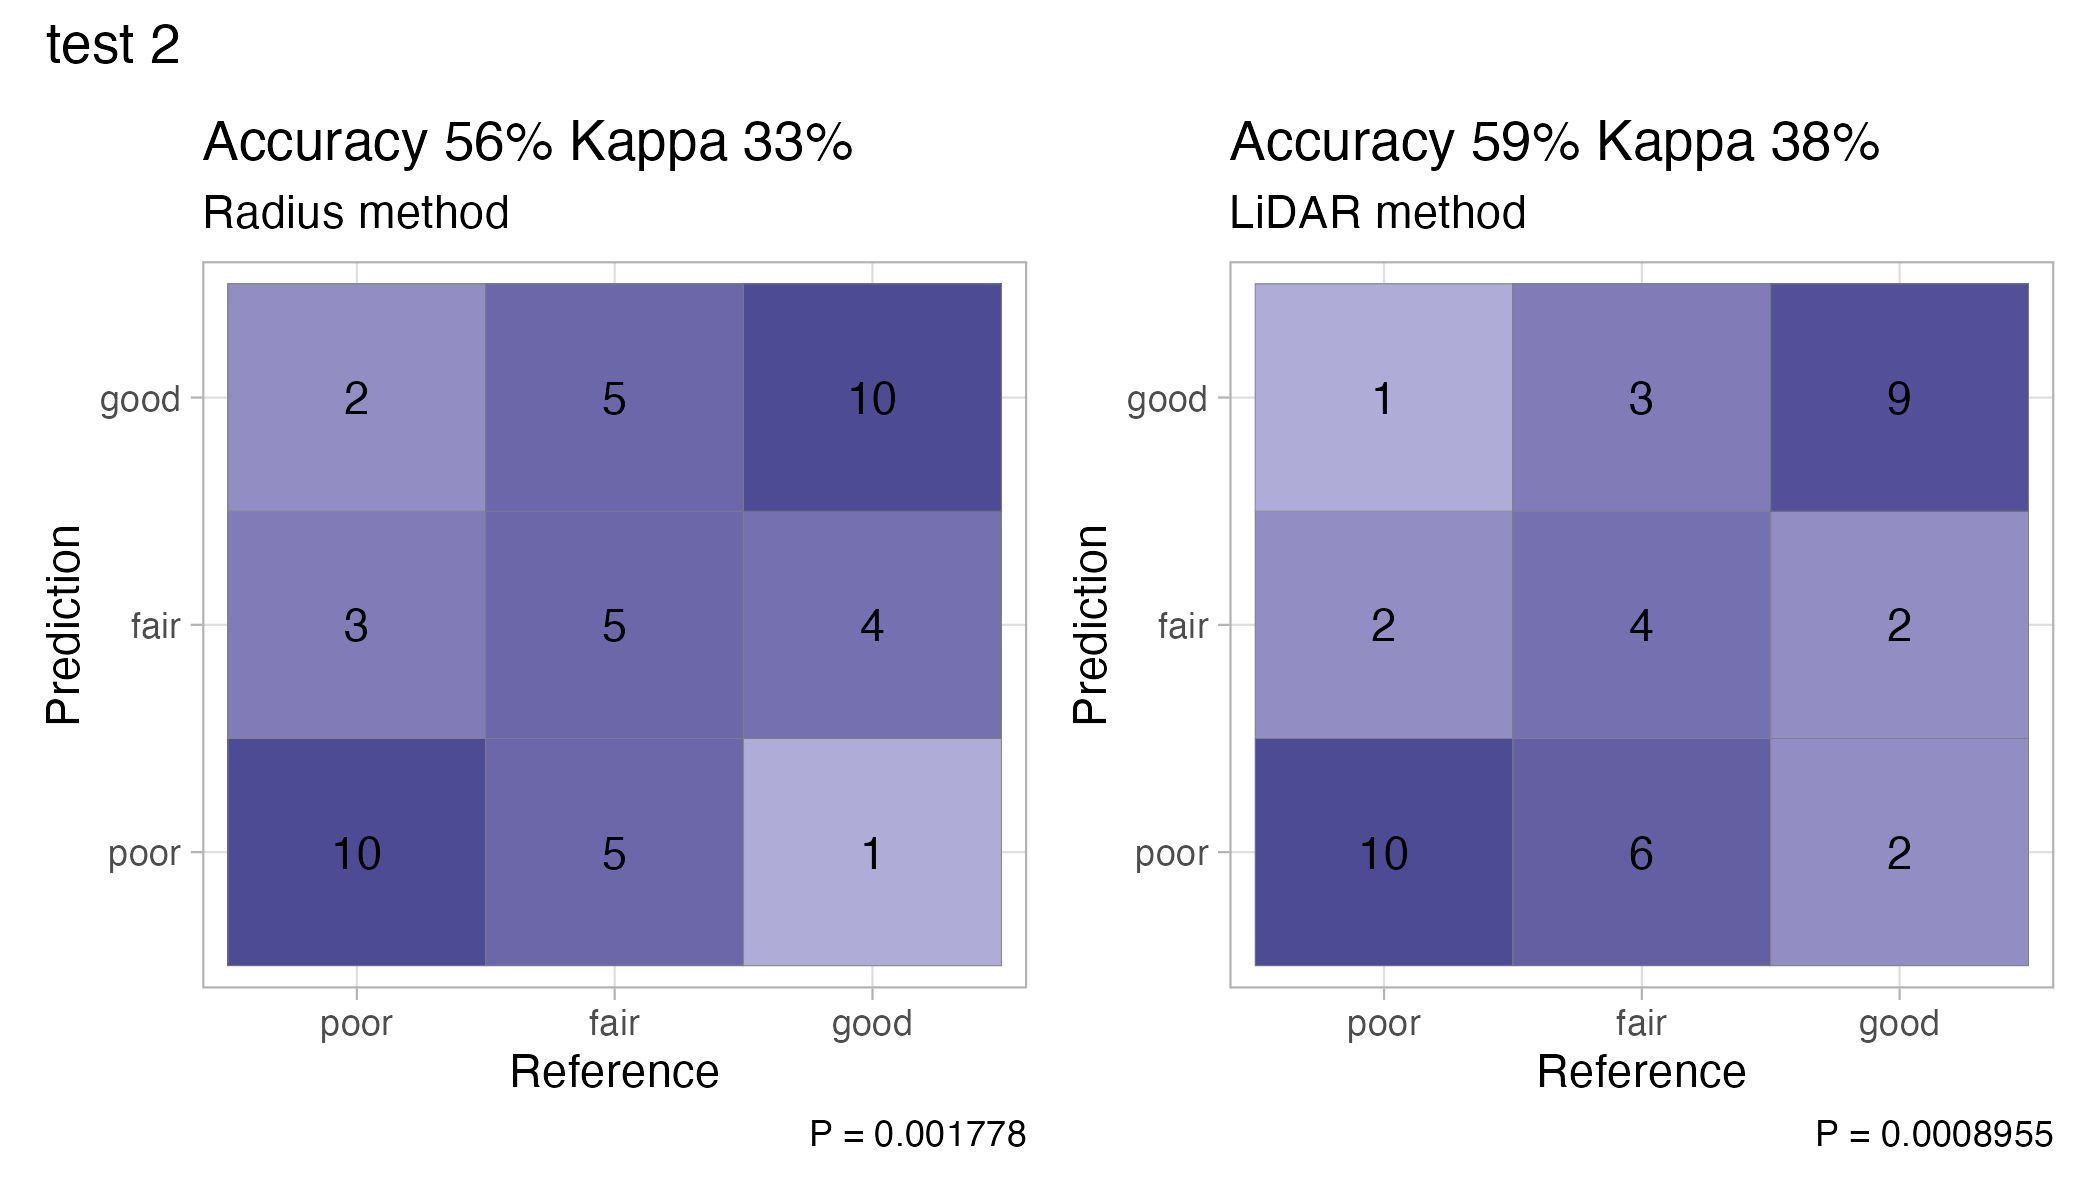
\includegraphics[width=0.85\linewidth]{figure/test2}
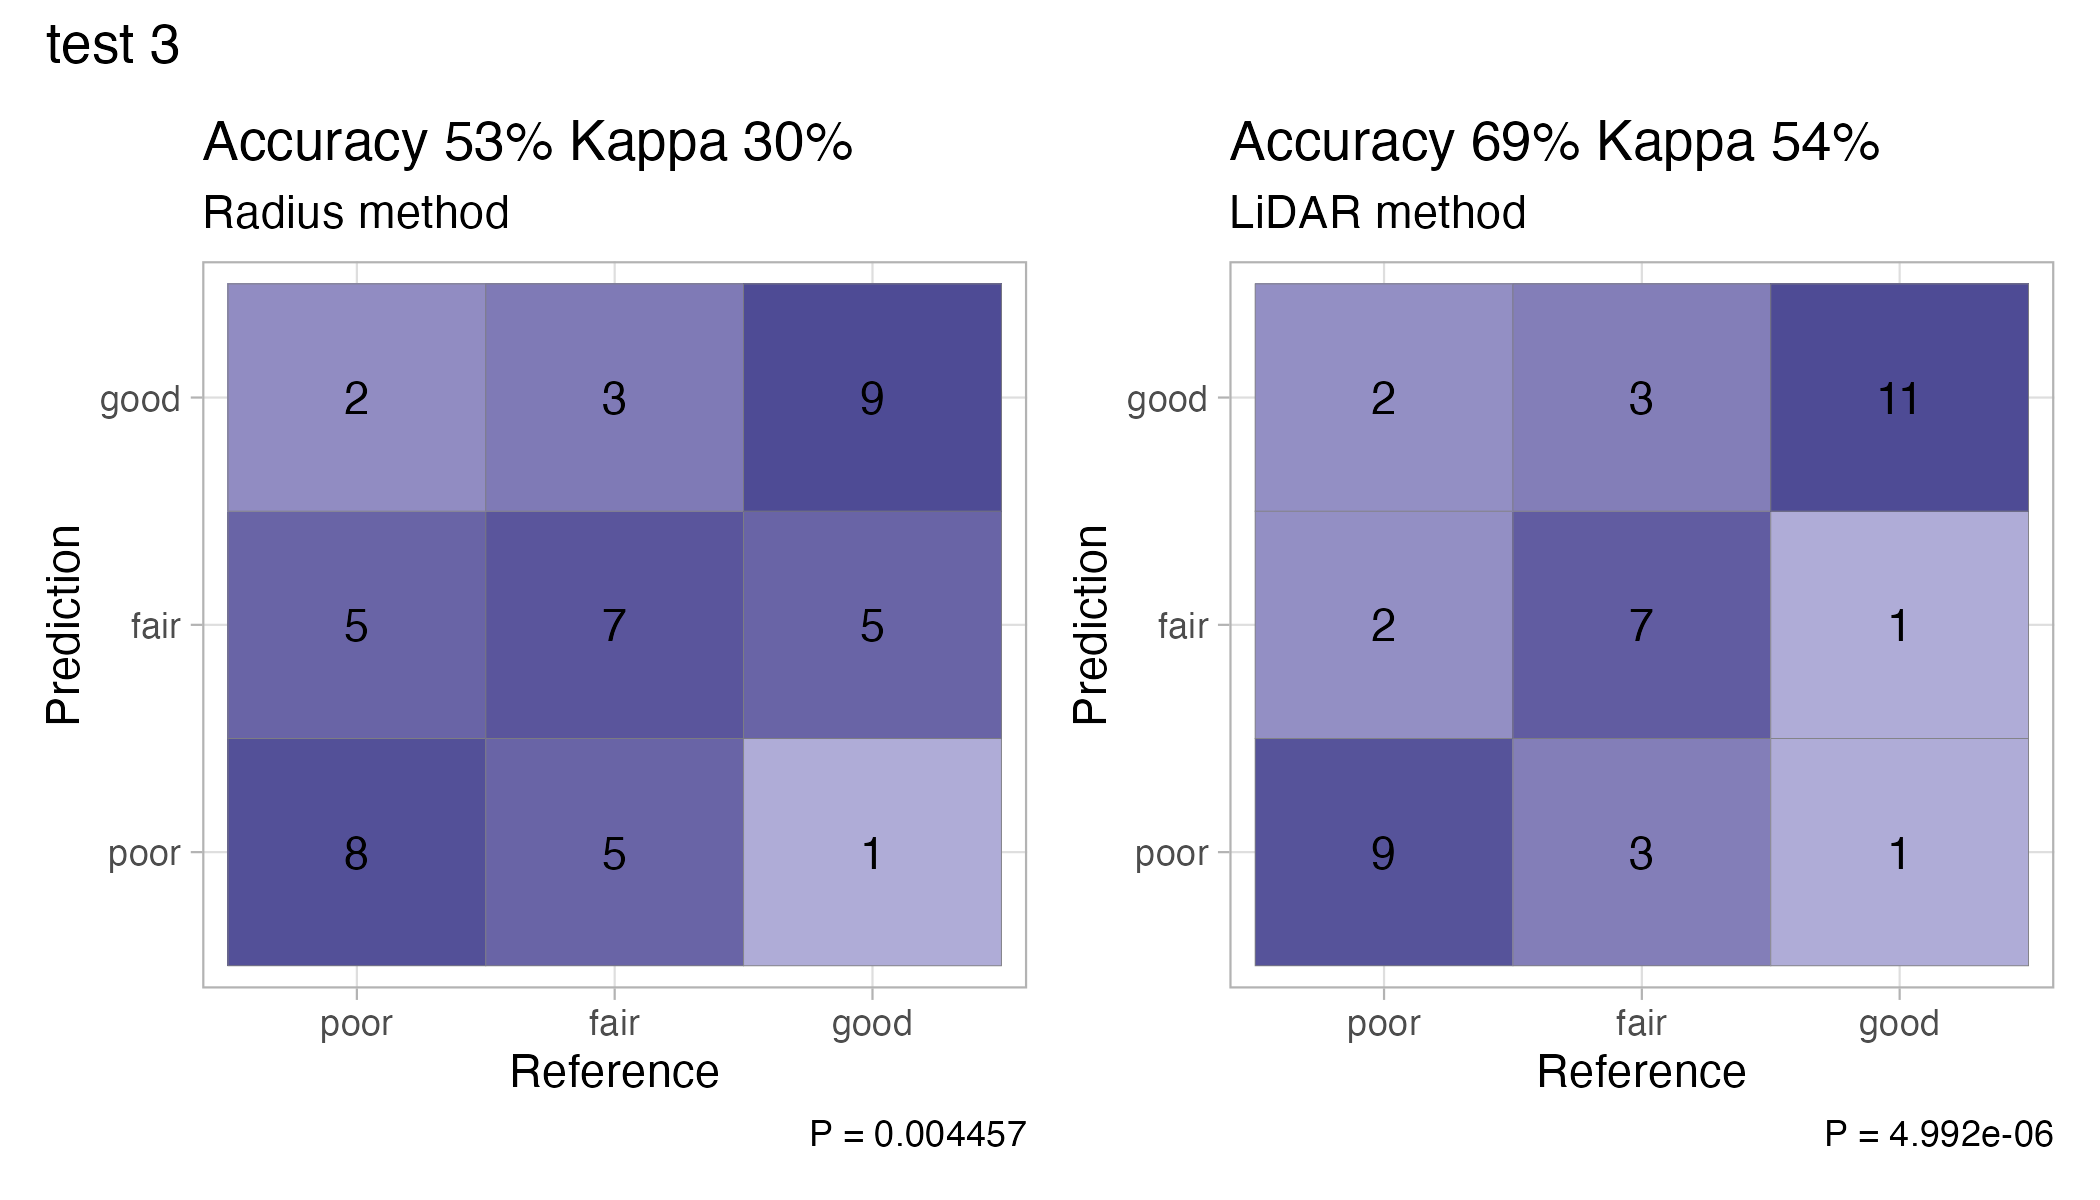
\includegraphics[width=0.85\linewidth]{figure/test3}
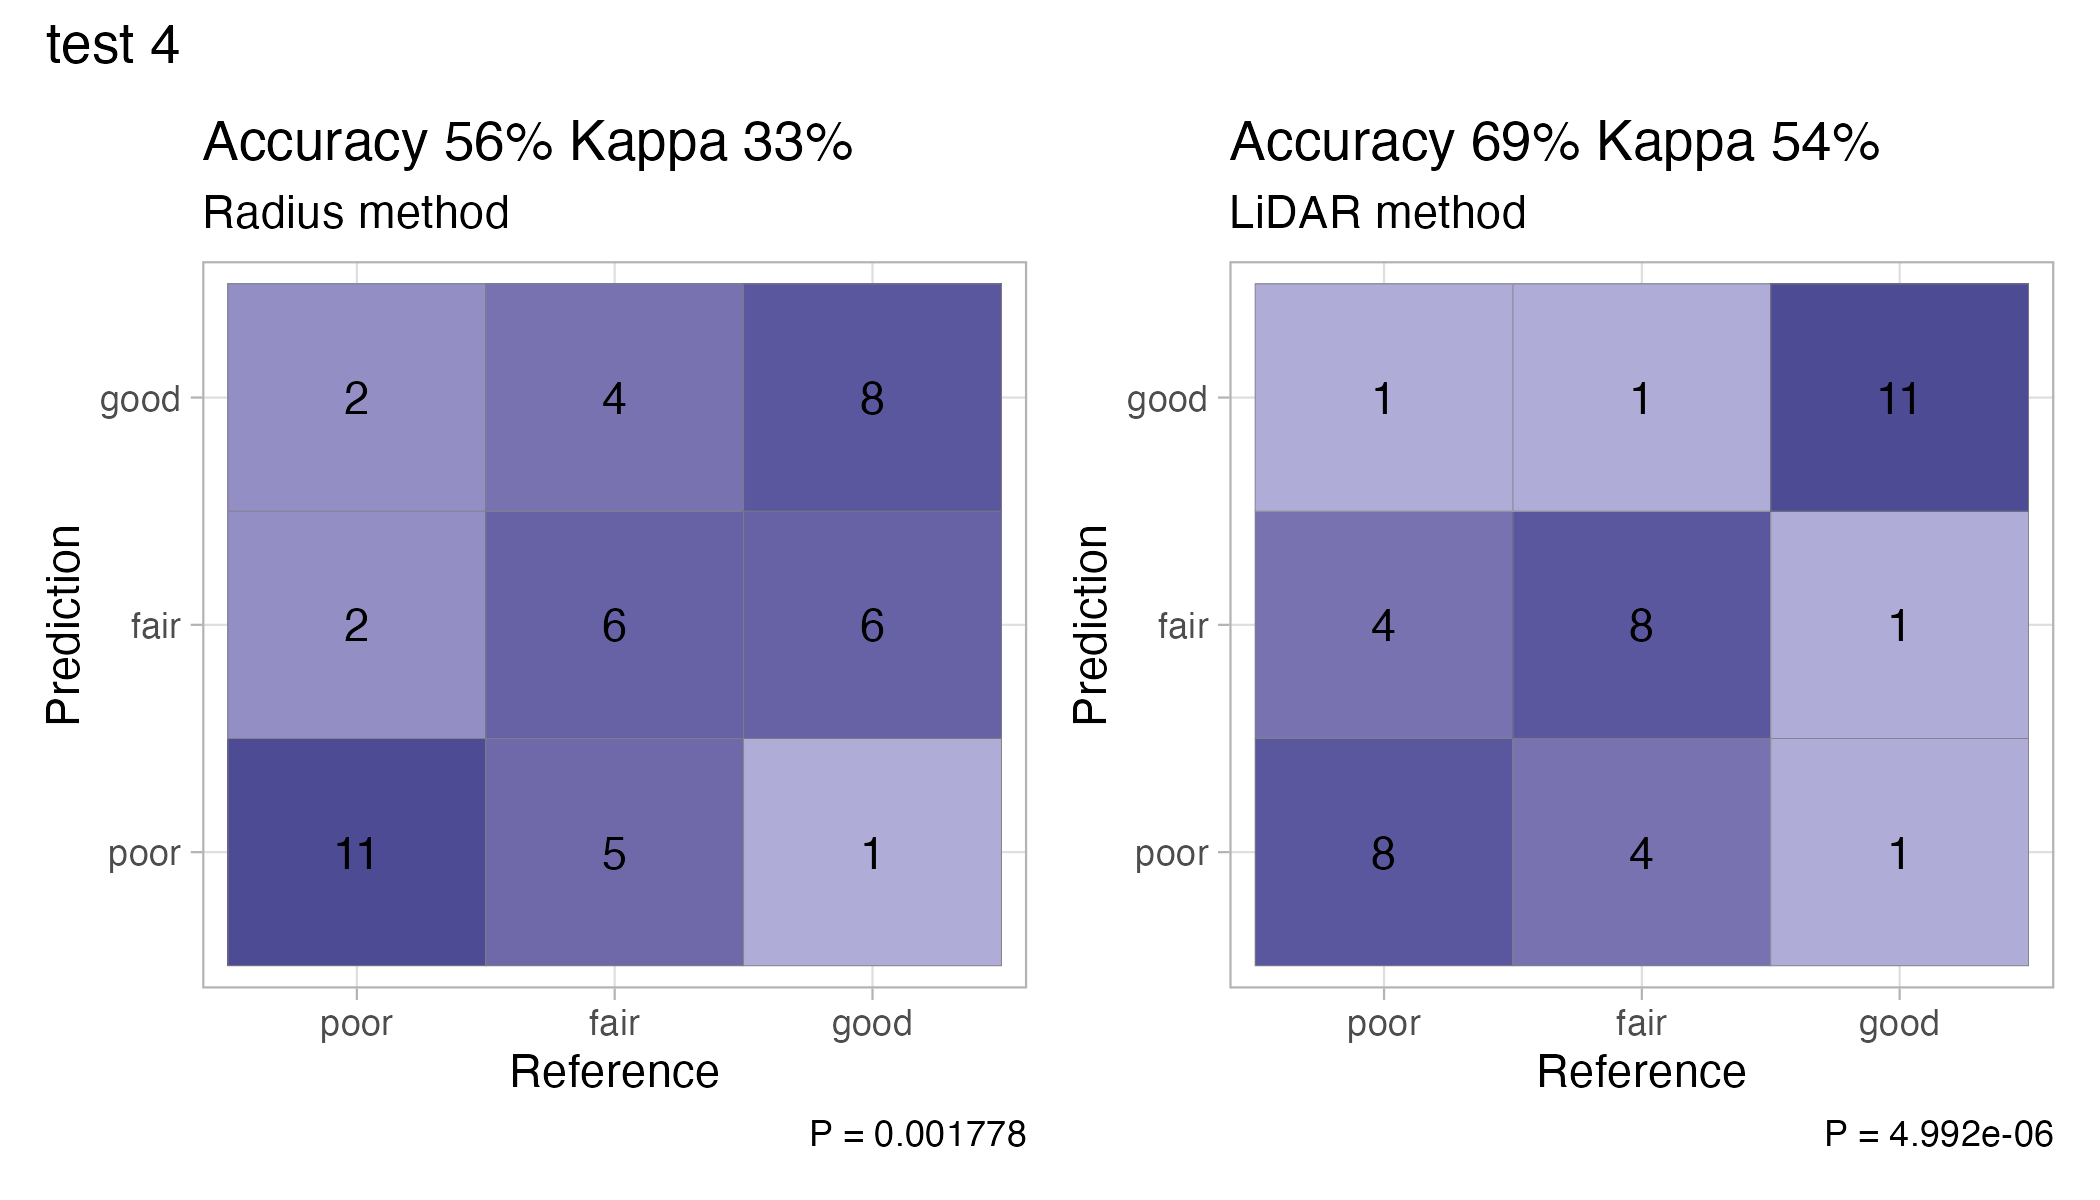
\includegraphics[width=0.85\linewidth]{figure/test4}
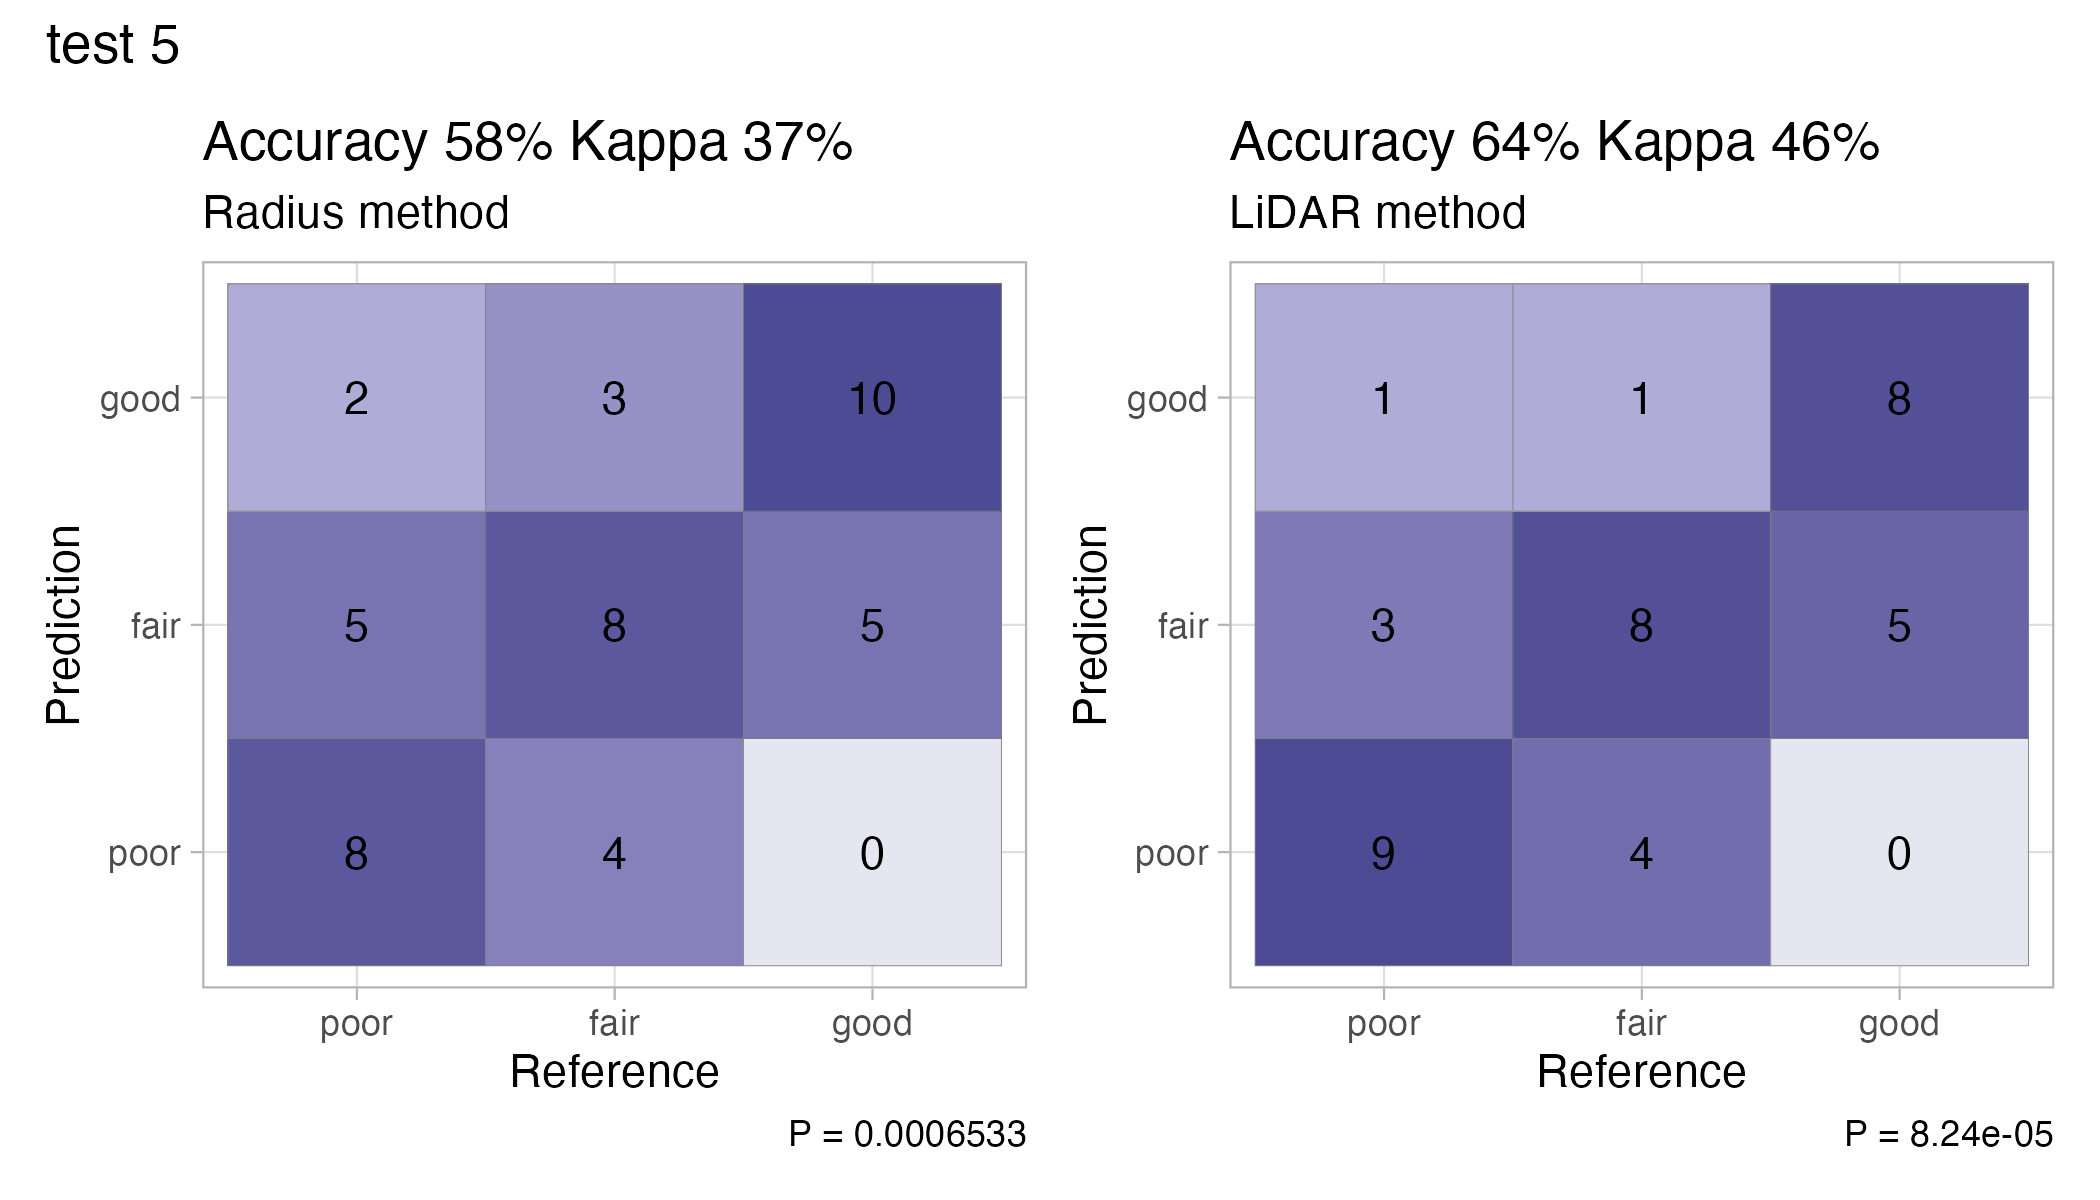
\includegraphics[width=0.85\linewidth]{figure/test5}
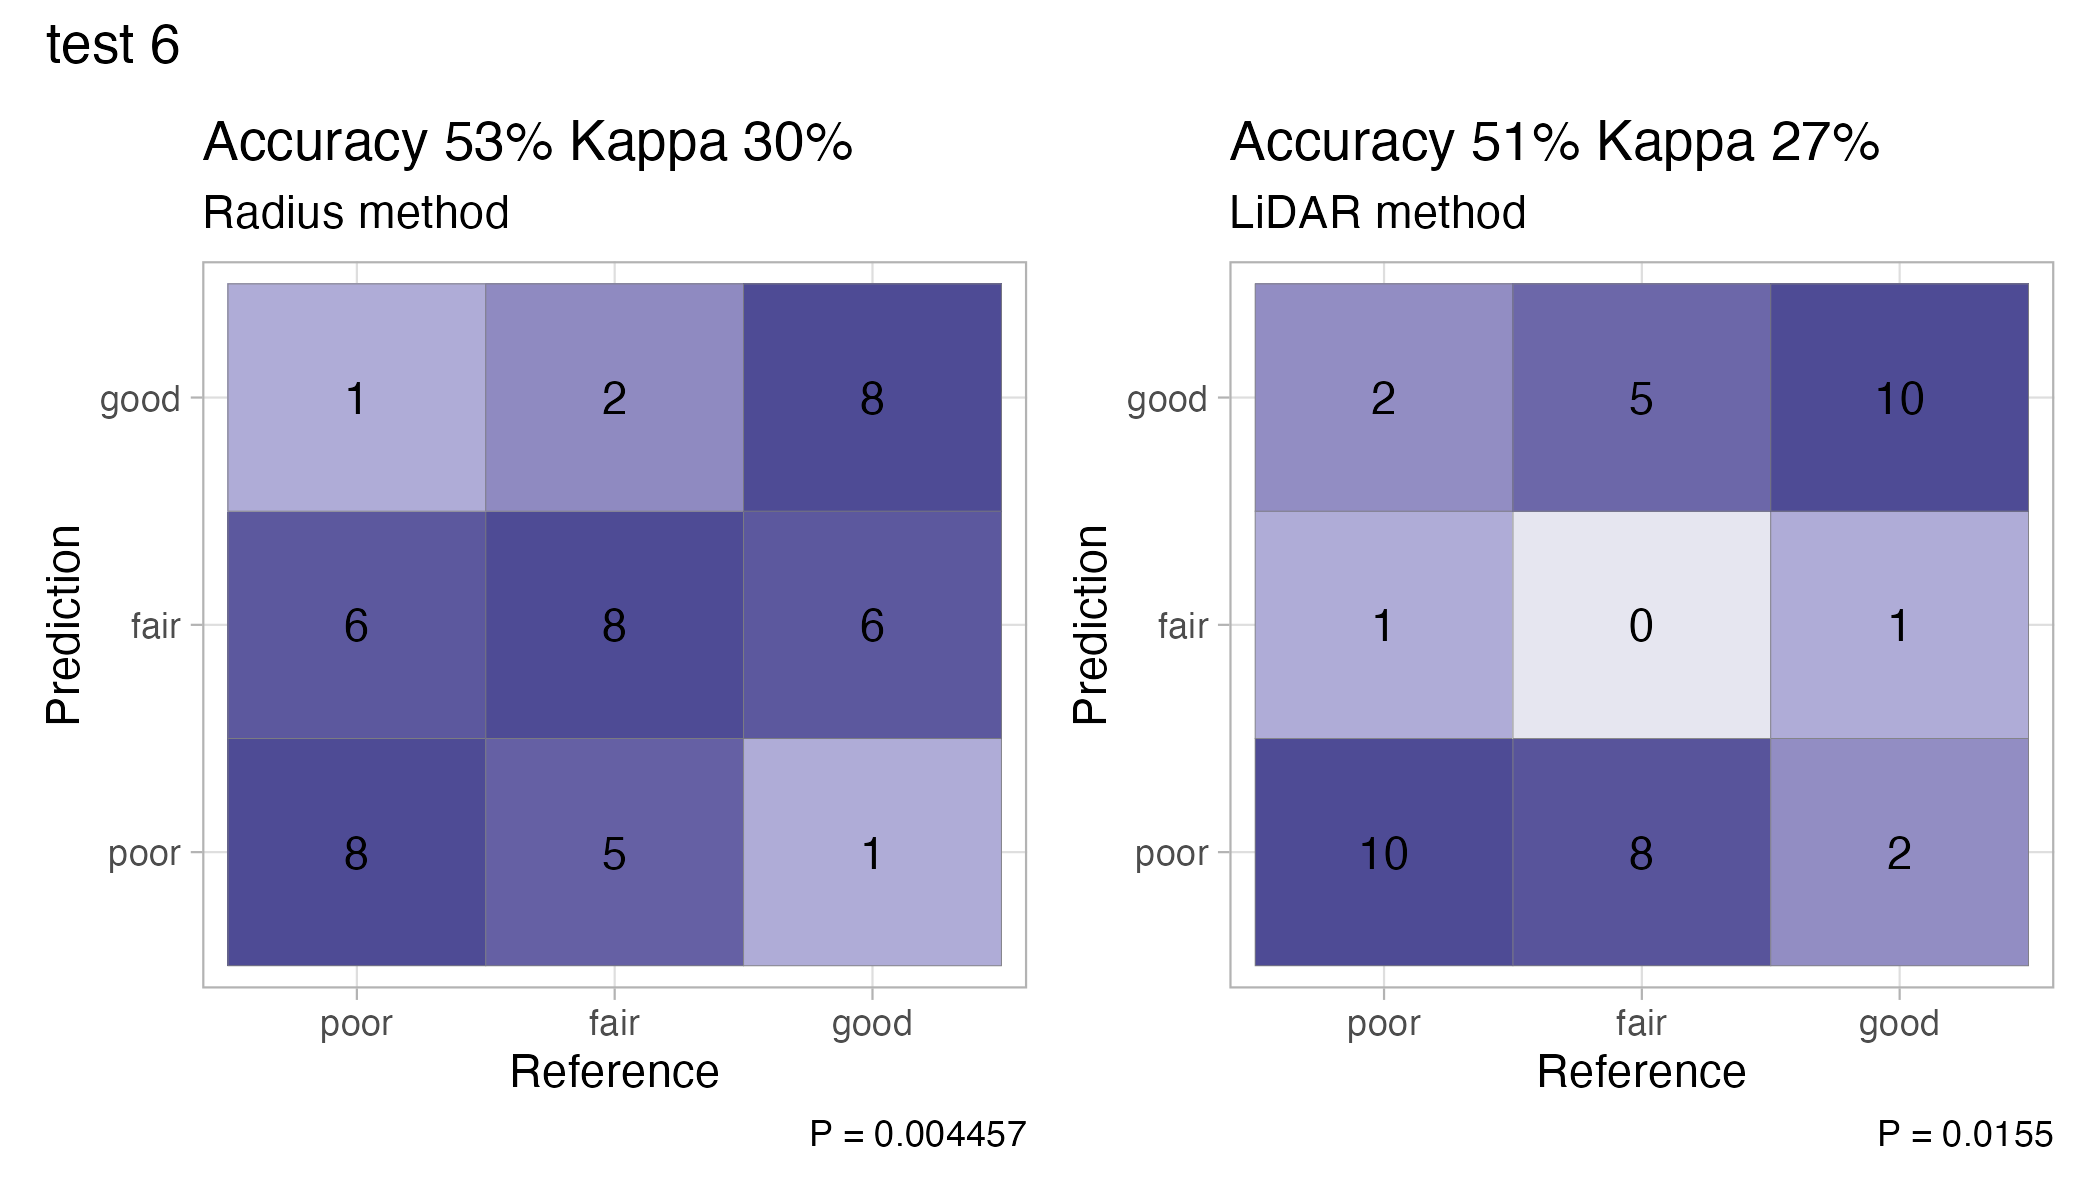
\includegraphics[width=0.85\linewidth]{figure/test6}

\hypertarget{code-chunks}{%
\chapter{Code}\label{code-chunks}}

This second appendix includes all of the R chunks of code that were hidden throughout the document to help with readability and/or setup.

\hypertarget{in-chapter-refdata-methods}{%
\section{\texorpdfstring{\textbf{In Chapter} \ref{data-methods}\textbf{:}}{In Chapter \ref{data-methods}:}}\label{in-chapter-refdata-methods}}

\hypertarget{portland-tree-inventory-counts-and-calculations}{%
\subsection*{Portland Tree Inventory counts and calculations}\label{portland-tree-inventory-counts-and-calculations}}
\addcontentsline{toc}{subsection}{Portland Tree Inventory counts and calculations}

\footnotesize
\begin{Shaded}
\begin{Highlighting}[]
\NormalTok{street\_counts }\OtherTok{\textless{}{-}} \FunctionTok{get\_pdxTrees\_streets}\NormalTok{() }\SpecialCharTok{\%\textgreater{}\%}
    \FunctionTok{filter}\NormalTok{(Species }\SpecialCharTok{\%in\%} \FunctionTok{c}\NormalTok{(}\StringTok{"ACMA"}\NormalTok{, }\StringTok{"ACPL"}\NormalTok{, }\StringTok{"PSME"}\NormalTok{, }\StringTok{"THPL"}\NormalTok{)) }\SpecialCharTok{\%\textgreater{}\%}
    \FunctionTok{mutate}\NormalTok{(}\AttributeTok{year =} \FunctionTok{year}\NormalTok{(Inventory\_Date)) }\SpecialCharTok{\%\textgreater{}\%}
\NormalTok{    dplyr}\SpecialCharTok{::}\FunctionTok{select}\NormalTok{(Species, Scientific, year) }\SpecialCharTok{\%\textgreater{}\%}
    \FunctionTok{add\_count}\NormalTok{(Species, year) }\SpecialCharTok{\%\textgreater{}\%}
    \FunctionTok{distinct}\NormalTok{() }\SpecialCharTok{\%\textgreater{}\%}
    \FunctionTok{group\_by}\NormalTok{(Species) }\SpecialCharTok{\%\textgreater{}\%}
    \FunctionTok{mutate}\NormalTok{(}\AttributeTok{Total =} \FunctionTok{sum}\NormalTok{(n)) }\SpecialCharTok{\%\textgreater{}\%}
    \FunctionTok{rename}\NormalTok{(}\AttributeTok{Count\_2016 =}\NormalTok{ n) }\SpecialCharTok{\%\textgreater{}\%}
    \FunctionTok{filter}\NormalTok{(year }\SpecialCharTok{==} \DecValTok{2016}\NormalTok{) }\SpecialCharTok{\%\textgreater{}\%}
\NormalTok{    dplyr}\SpecialCharTok{::}\FunctionTok{select}\NormalTok{(}\SpecialCharTok{{-}}\NormalTok{year)}
\NormalTok{park\_counts }\OtherTok{\textless{}{-}} \FunctionTok{get\_pdxTrees\_parks}\NormalTok{() }\SpecialCharTok{\%\textgreater{}\%}
    \FunctionTok{filter}\NormalTok{(Species }\SpecialCharTok{\%in\%} \FunctionTok{c}\NormalTok{(}\StringTok{"ACMA"}\NormalTok{, }\StringTok{"ACPL"}\NormalTok{, }\StringTok{"PSME"}\NormalTok{, }\StringTok{"THPL"}\NormalTok{)) }\SpecialCharTok{\%\textgreater{}\%}
    \FunctionTok{mutate}\NormalTok{(}\AttributeTok{year =} \FunctionTok{year}\NormalTok{(Inventory\_Date)) }\SpecialCharTok{\%\textgreater{}\%}
\NormalTok{    dplyr}\SpecialCharTok{::}\FunctionTok{select}\NormalTok{(Species, Scientific\_Name, year) }\SpecialCharTok{\%\textgreater{}\%}
    \FunctionTok{add\_count}\NormalTok{(Species, year) }\SpecialCharTok{\%\textgreater{}\%}
    \FunctionTok{distinct}\NormalTok{() }\SpecialCharTok{\%\textgreater{}\%}
    \FunctionTok{group\_by}\NormalTok{(Species) }\SpecialCharTok{\%\textgreater{}\%}
    \FunctionTok{mutate}\NormalTok{(}\AttributeTok{Total =} \FunctionTok{sum}\NormalTok{(n)) }\SpecialCharTok{\%\textgreater{}\%}
    \FunctionTok{rename}\NormalTok{(}\AttributeTok{Count\_2019 =}\NormalTok{ n) }\SpecialCharTok{\%\textgreater{}\%}
    \FunctionTok{filter}\NormalTok{(year }\SpecialCharTok{==} \DecValTok{2019}\NormalTok{) }\SpecialCharTok{\%\textgreater{}\%}
\NormalTok{    dplyr}\SpecialCharTok{::}\FunctionTok{select}\NormalTok{(}\SpecialCharTok{{-}}\NormalTok{year)}
\end{Highlighting}
\end{Shaded}
\normalsize

\hypertarget{calculating-ndvi-from-satellite-imagery}{%
\subsection*{Calculating NDVI from satellite imagery}\label{calculating-ndvi-from-satellite-imagery}}
\addcontentsline{toc}{subsection}{Calculating NDVI from satellite imagery}

\footnotesize
\begin{Shaded}
\begin{Highlighting}[]
\NormalTok{import rasterio}
\NormalTok{import numpy}

\NormalTok{files }\OtherTok{=}\NormalTok{ [}\StringTok{"1"}\NormalTok{, }\StringTok{"2"}\NormalTok{, }\StringTok{"3"}\NormalTok{, }\StringTok{"4"}\NormalTok{] }\CommentTok{\# unique file identifiers}
\NormalTok{folder }\OtherTok{=} \StringTok{"ndvi\_calc\_thesis/files"} \CommentTok{\# folder with the raw files}
\NormalTok{date }\OtherTok{=} \StringTok{"20210726"} \CommentTok{\# product date}


\ControlFlowTok{for}\NormalTok{ i }\ControlFlowTok{in} \FunctionTok{range}\NormalTok{(}\FunctionTok{len}\NormalTok{(files))}\SpecialCharTok{:}
\NormalTok{    filenum }\OtherTok{=}\NormalTok{ files[i]}
\NormalTok{    image\_file }\OtherTok{=}\NormalTok{ folder}\SpecialCharTok{+}\StringTok{"/"}\SpecialCharTok{+}\NormalTok{date}\SpecialCharTok{+}\StringTok{"\_"}\SpecialCharTok{+}\NormalTok{filenum}\SpecialCharTok{+}\StringTok{"\_AnalyticMS.tif"}

\NormalTok{    metafile }\OtherTok{=}\NormalTok{ folder}\SpecialCharTok{+}\StringTok{"/"}\SpecialCharTok{+}\NormalTok{date}\SpecialCharTok{+}\StringTok{"\_"}\SpecialCharTok{+}\NormalTok{filenum}\SpecialCharTok{+}\StringTok{"\_AnalyticMS\_metadata.xml"}
    \FunctionTok{print}\NormalTok{(image\_file)}
    \FunctionTok{print}\NormalTok{(metafile)}

    \CommentTok{\# Load red and NIR bands {-} }
    \CommentTok{\# note all PlanetScope 4{-}band images have band order BGRN}

\NormalTok{    with }\FunctionTok{rasterio.open}\NormalTok{(image\_file) as src}\SpecialCharTok{:}
\NormalTok{        band\_red }\OtherTok{=} \FunctionTok{src.read}\NormalTok{(}\DecValTok{3}\NormalTok{)}

\NormalTok{    with }\FunctionTok{rasterio.open}\NormalTok{(image\_file) as src}\SpecialCharTok{:}
\NormalTok{        band\_nir }\OtherTok{=} \FunctionTok{src.read}\NormalTok{(}\DecValTok{4}\NormalTok{)}

\NormalTok{    from xml.dom import minidom}

\NormalTok{    xmldoc }\OtherTok{=} \FunctionTok{minidom.parse}\NormalTok{(metafile)}
\NormalTok{    nodes }\OtherTok{=} \FunctionTok{xmldoc.getElementsByTagName}\NormalTok{(}\StringTok{"ps:bandSpecificMetadata"}\NormalTok{)}

    \CommentTok{\# XML parser refers to bands by numbers 1{-}4}
\NormalTok{    coeffs }\OtherTok{=}\NormalTok{ \{\}}
    \ControlFlowTok{for}\NormalTok{ node }\ControlFlowTok{in}\NormalTok{ nodes}\SpecialCharTok{:}
\NormalTok{        bn }\OtherTok{=} \FunctionTok{node.getElementsByTagName}\NormalTok{(}\StringTok{"ps:bandNumber"}\NormalTok{)[}\DecValTok{0}\NormalTok{].firstChild.data}
        \ControlFlowTok{if}\NormalTok{ bn }\ControlFlowTok{in}\NormalTok{ [}\StringTok{\textquotesingle{}1\textquotesingle{}}\NormalTok{, }\StringTok{\textquotesingle{}2\textquotesingle{}}\NormalTok{, }\StringTok{\textquotesingle{}3\textquotesingle{}}\NormalTok{, }\StringTok{\textquotesingle{}4\textquotesingle{}}\NormalTok{]}\SpecialCharTok{:}
\NormalTok{            i }\OtherTok{=} \FunctionTok{int}\NormalTok{(bn)}
\NormalTok{            value }\OtherTok{=} \FunctionTok{node.getElementsByTagName}\NormalTok{(}\StringTok{"ps:reflectanceCoefficient"}\NormalTok{)[}\DecValTok{0}\NormalTok{].firstChild.data}
\NormalTok{            coeffs[i] }\OtherTok{=} \FunctionTok{float}\NormalTok{(value)}

    \CommentTok{\# Multiply by corresponding coefficients}
\NormalTok{    band\_red }\OtherTok{=}\NormalTok{ band\_red }\SpecialCharTok{*}\NormalTok{ coeffs[}\DecValTok{3}\NormalTok{]}
\NormalTok{    band\_nir }\OtherTok{=}\NormalTok{ band\_nir }\SpecialCharTok{*}\NormalTok{ coeffs[}\DecValTok{4}\NormalTok{]}

    \CommentTok{\# Allow division by zero}
    \FunctionTok{numpy.seterr}\NormalTok{(}\AttributeTok{divide=}\StringTok{\textquotesingle{}ignore\textquotesingle{}}\NormalTok{, }\AttributeTok{invalid=}\StringTok{\textquotesingle{}ignore\textquotesingle{}}\NormalTok{)}

    \CommentTok{\# Calculate NDVI}
\NormalTok{    ndvi }\OtherTok{=}\NormalTok{ (}\FunctionTok{band\_nir.astype}\NormalTok{(float) }\SpecialCharTok{{-}} \FunctionTok{band\_red.astype}\NormalTok{(float)) }\SpecialCharTok{/}\NormalTok{ (band\_nir }\SpecialCharTok{+}\NormalTok{ band\_red)}

    \CommentTok{\# Set spatial characteristics of the output object to mirror the input}
\NormalTok{    kwargs }\OtherTok{=}\NormalTok{ src.meta}
    \FunctionTok{kwargs.update}\NormalTok{(}
        \AttributeTok{dtype=}\NormalTok{rasterio.float32,}
        \AttributeTok{count=}\DecValTok{1}\NormalTok{)}
    
    \CommentTok{\# Set name for new NDVI file}
\NormalTok{    newfile }\OtherTok{=}\NormalTok{ folder }\SpecialCharTok{+} \StringTok{\textquotesingle{}/ndvi\_\textquotesingle{}} \SpecialCharTok{+}\NormalTok{ date }\SpecialCharTok{+} \StringTok{"\_"} \SpecialCharTok{+}\NormalTok{ filenum }\SpecialCharTok{+} \StringTok{\textquotesingle{}.tif\textquotesingle{}}

    \CommentTok{\# Create the file}
\NormalTok{    with }\FunctionTok{rasterio.open}\NormalTok{(newfile, }\StringTok{\textquotesingle{}w\textquotesingle{}}\NormalTok{, }\SpecialCharTok{**}\NormalTok{kwargs) as dst}\SpecialCharTok{:}
        \FunctionTok{dst.write\_band}\NormalTok{(}\DecValTok{1}\NormalTok{, }\FunctionTok{ndvi.astype}\NormalTok{(rasterio.float32))}
\end{Highlighting}
\end{Shaded}
\normalsize

\hypertarget{lidar-canopy-delineation}{%
\subsection*{LiDAR canopy delineation}\label{lidar-canopy-delineation}}
\addcontentsline{toc}{subsection}{LiDAR canopy delineation}

\footnotesize
\begin{Shaded}
\begin{Highlighting}[]
\FunctionTok{library}\NormalTok{(rgdal)}
\FunctionTok{library}\NormalTok{(imager)}
\FunctionTok{library}\NormalTok{(raster)}
\FunctionTok{library}\NormalTok{(ForestTools)}
\FunctionTok{options}\NormalTok{(}\AttributeTok{rgdal\_show\_exportToProj4\_warnings =} \StringTok{"none"}\NormalTok{)}
\DocumentationTok{\#\# Loading raster data}
\NormalTok{EML\_CHM }\OtherTok{\textless{}{-}} \FunctionTok{raster}\NormalTok{(}\StringTok{"\textasciitilde{}Desktop/thesis\_data/lidar\_crown/clipped\_lidar.tif"}\NormalTok{)}
\DocumentationTok{\#\# Loading tree points}
\NormalTok{all\_ttops }\OtherTok{\textless{}{-}} \FunctionTok{shapefile}\NormalTok{(}\StringTok{"\textasciitilde{}Desktop/thesis\_data/lidar\_crown/all\_tree\_points\_for\_delin.tif"}\NormalTok{)}
\CommentTok{\# delineate tree crowns inputs: my tree points, LiDAR data}
\NormalTok{crownsPoly }\OtherTok{\textless{}{-}} \FunctionTok{mcws}\NormalTok{(}\AttributeTok{treetops =}\NormalTok{ all\_ttops, }\AttributeTok{CHM =}\NormalTok{ EML\_CHM, }\AttributeTok{format =} \StringTok{"polygons"}\NormalTok{,}
    \AttributeTok{minHeight =} \DecValTok{20}\NormalTok{, }\AttributeTok{verbose =} \ConstantTok{TRUE}\NormalTok{)}
\CommentTok{\# export file}
\FunctionTok{writeOGR}\NormalTok{(crownsPoly, }\StringTok{"\textasciitilde{}/Desktop/thesis\_data/lidar\_crown"}\NormalTok{, }\StringTok{"canopy\_delin\_polygons\_poly"}\NormalTok{,}
    \AttributeTok{driver =} \StringTok{"ESRI Shapefile"}\NormalTok{)}
\end{Highlighting}
\end{Shaded}
\normalsize

\hypertarget{in-chapter-refresults}{%
\section{\texorpdfstring{\textbf{In Chapter} \ref{results}\textbf{:}}{In Chapter \ref{results}:}}\label{in-chapter-refresults}}

\hypertarget{model-for-tree-height-and-canopy-width}{%
\subsection*{Model for Tree Height and Canopy Width}\label{model-for-tree-height-and-canopy-width}}
\addcontentsline{toc}{subsection}{Model for Tree Height and Canopy Width}

\footnotesize
\begin{Shaded}
\begin{Highlighting}[]
\CommentTok{\# load park data, filter to relevant species, and get}
\CommentTok{\# average crown width.}
\NormalTok{my\_park }\OtherTok{\textless{}{-}}\NormalTok{ pdxTrees}\SpecialCharTok{::}\FunctionTok{get\_pdxTrees\_parks}\NormalTok{() }\SpecialCharTok{\%\textgreater{}\%}
    \FunctionTok{filter}\NormalTok{(Species }\SpecialCharTok{\%in\%} \FunctionTok{c}\NormalTok{(}\StringTok{"ACPL"}\NormalTok{, }\StringTok{"THPL"}\NormalTok{, }\StringTok{"PSME"}\NormalTok{, }\StringTok{"ACMA"}\NormalTok{)) }\SpecialCharTok{\%\textgreater{}\%}
    \FunctionTok{mutate}\NormalTok{(}\AttributeTok{crown\_width =}\NormalTok{ (Crown\_Width\_EW }\SpecialCharTok{+}\NormalTok{ Crown\_Width\_NS)}\SpecialCharTok{/}\DecValTok{2}\NormalTok{)}
\CommentTok{\# create model for heights}
\NormalTok{heights }\OtherTok{\textless{}{-}} \FunctionTok{lm}\NormalTok{(Tree\_Height }\SpecialCharTok{\textasciitilde{}} \FunctionTok{poly}\NormalTok{(DBH, }\AttributeTok{degree =} \DecValTok{3}\NormalTok{, }\AttributeTok{raw =}\NormalTok{ T) }\SpecialCharTok{*}
\NormalTok{    Species, }\AttributeTok{data =}\NormalTok{ my\_park)}
\CommentTok{\# create model for crown width}
\NormalTok{cr\_width }\OtherTok{\textless{}{-}} \FunctionTok{lm}\NormalTok{(crown\_width }\SpecialCharTok{\textasciitilde{}} \FunctionTok{poly}\NormalTok{(DBH, }\AttributeTok{degree =} \DecValTok{3}\NormalTok{, }\AttributeTok{raw =}\NormalTok{ T) }\SpecialCharTok{*}
\NormalTok{    Species, }\AttributeTok{data =}\NormalTok{ my\_park)}
\CommentTok{\# load street data, filter to relevant species}
\NormalTok{my\_street }\OtherTok{\textless{}{-}}\NormalTok{ pdxTrees}\SpecialCharTok{::}\FunctionTok{get\_pdxTrees\_streets}\NormalTok{() }\SpecialCharTok{\%\textgreater{}\%}
    \FunctionTok{filter}\NormalTok{(Species }\SpecialCharTok{\%in\%} \FunctionTok{c}\NormalTok{(}\StringTok{"ACPL"}\NormalTok{, }\StringTok{"THPL"}\NormalTok{, }\StringTok{"PSME"}\NormalTok{, }\StringTok{"ACMA"}\NormalTok{))}
\CommentTok{\# run street trees through both models}
\NormalTok{my\_street }\OtherTok{\textless{}{-}}\NormalTok{ my\_street }\SpecialCharTok{\%\textgreater{}\%}
    \FunctionTok{mutate}\NormalTok{(}\AttributeTok{width\_preds =} \FunctionTok{predict}\NormalTok{(cr\_width, my\_street, }\AttributeTok{se.fit =} \ConstantTok{FALSE}\NormalTok{),}
        \AttributeTok{height\_preds =} \FunctionTok{predict}\NormalTok{(heights, my\_street, }\AttributeTok{se.fit =}\NormalTok{ F))}
\CommentTok{\# export data file write\_csv(my\_street, \textquotesingle{}my\_street.csv\textquotesingle{})}
\CommentTok{\# graphing}
\NormalTok{p\_height\_model }\OtherTok{\textless{}{-}}\NormalTok{ my\_park }\SpecialCharTok{\%\textgreater{}\%}
    \FunctionTok{ggplot}\NormalTok{(}\FunctionTok{aes}\NormalTok{(}\AttributeTok{x =} \FunctionTok{sqrt}\NormalTok{(DBH), }\AttributeTok{y =}\NormalTok{ Tree\_Height, }\AttributeTok{color =}\NormalTok{ Species)) }\SpecialCharTok{+}
    \FunctionTok{geom\_point}\NormalTok{(}\AttributeTok{alpha =} \FloatTok{0.1}\NormalTok{) }\SpecialCharTok{+} \FunctionTok{scale\_color\_manual}\NormalTok{(}\AttributeTok{values =}\NormalTok{ species\_pal) }\SpecialCharTok{+}
    \FunctionTok{geom\_smooth}\NormalTok{(}\AttributeTok{method =} \StringTok{"lm"}\NormalTok{, }\AttributeTok{se =}\NormalTok{ F, }\AttributeTok{formula =}\NormalTok{ y }\SpecialCharTok{\textasciitilde{}} \FunctionTok{poly}\NormalTok{(x,}
        \AttributeTok{degree =} \DecValTok{3}\NormalTok{, }\AttributeTok{raw =}\NormalTok{ T)) }\SpecialCharTok{+} \FunctionTok{labs}\NormalTok{(}\AttributeTok{subtitle =} \StringTok{"Park trees"}\NormalTok{,}
    \AttributeTok{y =} \StringTok{"Tree Height Measurement"}\NormalTok{) }\SpecialCharTok{+} \FunctionTok{guides}\NormalTok{(}\AttributeTok{color =} \StringTok{"none"}\NormalTok{)}
\NormalTok{p\_width\_model }\OtherTok{\textless{}{-}}\NormalTok{ my\_park }\SpecialCharTok{\%\textgreater{}\%}
    \FunctionTok{ggplot}\NormalTok{(}\FunctionTok{aes}\NormalTok{(}\AttributeTok{x =} \FunctionTok{sqrt}\NormalTok{(DBH), }\AttributeTok{y =}\NormalTok{ crown\_width, }\AttributeTok{color =}\NormalTok{ Species)) }\SpecialCharTok{+}
    \FunctionTok{geom\_point}\NormalTok{(}\AttributeTok{alpha =} \FloatTok{0.1}\NormalTok{) }\SpecialCharTok{+} \FunctionTok{scale\_color\_manual}\NormalTok{(}\AttributeTok{values =}\NormalTok{ species\_pal) }\SpecialCharTok{+}
    \FunctionTok{geom\_smooth}\NormalTok{(}\AttributeTok{method =} \StringTok{"lm"}\NormalTok{, }\AttributeTok{se =}\NormalTok{ F, }\AttributeTok{formula =}\NormalTok{ y }\SpecialCharTok{\textasciitilde{}} \FunctionTok{poly}\NormalTok{(x,}
        \AttributeTok{degree =} \DecValTok{3}\NormalTok{, }\AttributeTok{raw =}\NormalTok{ T)) }\SpecialCharTok{+} \FunctionTok{labs}\NormalTok{(}\AttributeTok{subtitle =} \StringTok{"Park trees"}\NormalTok{,}
    \AttributeTok{y =} \StringTok{"Canopy Width Measurement"}\NormalTok{) }\SpecialCharTok{+} \FunctionTok{guides}\NormalTok{(}\AttributeTok{color =} \StringTok{"none"}\NormalTok{)}
\NormalTok{s\_height\_preds }\OtherTok{\textless{}{-}}\NormalTok{ my\_street }\SpecialCharTok{\%\textgreater{}\%}
    \FunctionTok{ggplot}\NormalTok{(}\FunctionTok{aes}\NormalTok{(}\AttributeTok{x =} \FunctionTok{sqrt}\NormalTok{(DBH), }\AttributeTok{y =}\NormalTok{ height\_preds, }\AttributeTok{color =}\NormalTok{ Species)) }\SpecialCharTok{+}
    \FunctionTok{geom\_point}\NormalTok{(}\AttributeTok{alpha =} \FloatTok{0.3}\NormalTok{) }\SpecialCharTok{+} \FunctionTok{scale\_color\_manual}\NormalTok{(}\AttributeTok{values =}\NormalTok{ species\_pal) }\SpecialCharTok{+}
    \FunctionTok{labs}\NormalTok{(}\AttributeTok{subtitle =} \StringTok{"Street trees"}\NormalTok{, }\AttributeTok{y =} \StringTok{"Tree Height Prediction"}\NormalTok{)}
\NormalTok{s\_width\_preds }\OtherTok{\textless{}{-}}\NormalTok{ my\_street }\SpecialCharTok{\%\textgreater{}\%}
    \FunctionTok{ggplot}\NormalTok{(}\FunctionTok{aes}\NormalTok{(}\AttributeTok{x =} \FunctionTok{sqrt}\NormalTok{(DBH), }\AttributeTok{y =}\NormalTok{ width\_preds, }\AttributeTok{color =}\NormalTok{ Species)) }\SpecialCharTok{+}
    \FunctionTok{geom\_point}\NormalTok{(}\AttributeTok{alpha =} \FloatTok{0.3}\NormalTok{) }\SpecialCharTok{+} \FunctionTok{scale\_color\_manual}\NormalTok{(}\AttributeTok{values =}\NormalTok{ species\_pal) }\SpecialCharTok{+}
    \FunctionTok{labs}\NormalTok{(}\AttributeTok{subtitle =} \StringTok{"Street trees"}\NormalTok{, }\AttributeTok{y =} \StringTok{"Canopy Width Prediction"}\NormalTok{)}
\end{Highlighting}
\end{Shaded}
\normalsize

\hypertarget{point-method-modeling}{%
\subsection*{Point Method Modeling}\label{point-method-modeling}}
\addcontentsline{toc}{subsection}{Point Method Modeling}

\footnotesize
\begin{Shaded}
\begin{Highlighting}[]
\NormalTok{point\_all }\OtherTok{\textless{}{-}} \FunctionTok{polr}\NormalTok{(health\_rat }\SpecialCharTok{\textasciitilde{}}\NormalTok{ sample\_ndvi, }\AttributeTok{Hess =} \ConstantTok{TRUE}\NormalTok{, }\AttributeTok{data =}\NormalTok{ cnh\_point)}
\NormalTok{point\_all\_preds }\OtherTok{\textless{}{-}} \FunctionTok{predict}\NormalTok{(point\_all, cnh\_point)}
\NormalTok{cfm\_p\_all }\OtherTok{\textless{}{-}} \FunctionTok{confusionMatrix}\NormalTok{(point\_all\_preds, cnh\_point}\SpecialCharTok{$}\NormalTok{health\_rat)}
\NormalTok{p\_all }\OtherTok{\textless{}{-}} \FunctionTok{ggplotConfusionMatrix}\NormalTok{(cfm\_p\_all) }\SpecialCharTok{+} \FunctionTok{labs}\NormalTok{(}\AttributeTok{subtitle =} \StringTok{"health rating \textasciitilde{} NDVI"}\NormalTok{)}
\NormalTok{brant}\SpecialCharTok{::}\FunctionTok{brant}\NormalTok{(point\_all)}
\NormalTok{point\_type }\OtherTok{\textless{}{-}} \FunctionTok{polr}\NormalTok{(health\_rat }\SpecialCharTok{\textasciitilde{}}\NormalTok{ sample\_ndvi }\SpecialCharTok{*}\NormalTok{ tree\_type, }\AttributeTok{Hess =} \ConstantTok{TRUE}\NormalTok{,}
    \AttributeTok{data =}\NormalTok{ cnh\_point)}
\NormalTok{point\_type\_preds }\OtherTok{\textless{}{-}} \FunctionTok{predict}\NormalTok{(point\_type, cnh\_point)}
\NormalTok{cfm\_p\_type }\OtherTok{\textless{}{-}} \FunctionTok{confusionMatrix}\NormalTok{(point\_type\_preds, cnh\_point}\SpecialCharTok{$}\NormalTok{health\_rat)}
\NormalTok{p\_type }\OtherTok{\textless{}{-}} \FunctionTok{ggplotConfusionMatrix}\NormalTok{(cfm\_p\_type) }\SpecialCharTok{+} \FunctionTok{labs}\NormalTok{(}\AttributeTok{subtitle =} \StringTok{"health rating \textasciitilde{} NDVI * tree type"}\NormalTok{)}
\NormalTok{brant}\SpecialCharTok{::}\FunctionTok{brant}\NormalTok{(point\_type)}
\NormalTok{point\_species }\OtherTok{\textless{}{-}} \FunctionTok{polr}\NormalTok{(health\_rat }\SpecialCharTok{\textasciitilde{}}\NormalTok{ sample\_ndvi }\SpecialCharTok{*}\NormalTok{ species, }\AttributeTok{Hess =} \ConstantTok{TRUE}\NormalTok{,}
    \AttributeTok{data =}\NormalTok{ cnh\_point)}
\NormalTok{point\_species\_preds }\OtherTok{\textless{}{-}} \FunctionTok{predict}\NormalTok{(point\_species, cnh\_point)}
\NormalTok{cfm\_p\_species }\OtherTok{\textless{}{-}} \FunctionTok{confusionMatrix}\NormalTok{(point\_species\_preds, cnh\_point}\SpecialCharTok{$}\NormalTok{health\_rat)}
\NormalTok{p\_species }\OtherTok{\textless{}{-}} \FunctionTok{ggplotConfusionMatrix}\NormalTok{(cfm\_p\_species) }\SpecialCharTok{+} \FunctionTok{labs}\NormalTok{(}\AttributeTok{subtitle =} \StringTok{"health rating \textasciitilde{} NDVI * species"}\NormalTok{)}
\NormalTok{brant}\SpecialCharTok{::}\FunctionTok{brant}\NormalTok{(point\_species)}
\end{Highlighting}
\end{Shaded}
\normalsize

\hypertarget{radius-method-modeling}{%
\subsection*{Radius Method Modeling}\label{radius-method-modeling}}
\addcontentsline{toc}{subsection}{Radius Method Modeling}

\footnotesize
\begin{Shaded}
\begin{Highlighting}[]
\NormalTok{radius\_all }\OtherTok{\textless{}{-}} \FunctionTok{polr}\NormalTok{(health\_rat }\SpecialCharTok{\textasciitilde{}}\NormalTok{ sample\_ndvi, }\AttributeTok{Hess =} \ConstantTok{TRUE}\NormalTok{, }\AttributeTok{data =}\NormalTok{ cnh\_radius)}
\NormalTok{radius\_all\_preds }\OtherTok{\textless{}{-}} \FunctionTok{predict}\NormalTok{(radius\_all, cnh\_radius)}
\NormalTok{cfm\_r\_all }\OtherTok{\textless{}{-}} \FunctionTok{confusionMatrix}\NormalTok{(radius\_all\_preds, cnh\_radius}\SpecialCharTok{$}\NormalTok{health\_rat)}
\NormalTok{r\_all }\OtherTok{\textless{}{-}} \FunctionTok{ggplotConfusionMatrix}\NormalTok{(cfm\_r\_all) }\SpecialCharTok{+} \FunctionTok{labs}\NormalTok{(}\AttributeTok{subtitle =} \StringTok{"health rating \textasciitilde{} NDVI"}\NormalTok{)}
\NormalTok{radius\_type }\OtherTok{\textless{}{-}} \FunctionTok{polr}\NormalTok{(health\_rat }\SpecialCharTok{\textasciitilde{}}\NormalTok{ sample\_ndvi }\SpecialCharTok{*}\NormalTok{ tree\_type, }\AttributeTok{Hess =} \ConstantTok{TRUE}\NormalTok{,}
    \AttributeTok{data =}\NormalTok{ cnh\_radius)}
\NormalTok{radius\_type\_preds }\OtherTok{\textless{}{-}} \FunctionTok{predict}\NormalTok{(radius\_type, cnh\_radius)}
\NormalTok{cfm\_r\_type }\OtherTok{\textless{}{-}} \FunctionTok{confusionMatrix}\NormalTok{(radius\_type\_preds, cnh\_radius}\SpecialCharTok{$}\NormalTok{health\_rat)}
\NormalTok{r\_type }\OtherTok{\textless{}{-}} \FunctionTok{ggplotConfusionMatrix}\NormalTok{(cfm\_r\_type) }\SpecialCharTok{+} \FunctionTok{labs}\NormalTok{(}\AttributeTok{subtitle =} \StringTok{"health rating \textasciitilde{} NDVI * tree type"}\NormalTok{)}
\NormalTok{radius\_species }\OtherTok{\textless{}{-}} \FunctionTok{polr}\NormalTok{(health\_rat }\SpecialCharTok{\textasciitilde{}}\NormalTok{ sample\_ndvi }\SpecialCharTok{*}\NormalTok{ species, }\AttributeTok{Hess =} \ConstantTok{TRUE}\NormalTok{,}
    \AttributeTok{data =}\NormalTok{ cnh\_radius)}
\NormalTok{radius\_species\_preds }\OtherTok{\textless{}{-}} \FunctionTok{predict}\NormalTok{(radius\_species, cnh\_radius)}
\NormalTok{cfm\_r\_species }\OtherTok{\textless{}{-}} \FunctionTok{confusionMatrix}\NormalTok{(radius\_species\_preds, cnh\_radius}\SpecialCharTok{$}\NormalTok{health\_rat)}
\NormalTok{r\_species }\OtherTok{\textless{}{-}} \FunctionTok{ggplotConfusionMatrix}\NormalTok{(cfm\_r\_species) }\SpecialCharTok{+} \FunctionTok{labs}\NormalTok{(}\AttributeTok{subtitle =} \StringTok{"health rating \textasciitilde{} NDVI * species"}\NormalTok{)}
\end{Highlighting}
\end{Shaded}
\normalsize

\hypertarget{lidar-method-modeling}{%
\subsection*{LiDAR Method Modeling}\label{lidar-method-modeling}}
\addcontentsline{toc}{subsection}{LiDAR Method Modeling}

\footnotesize
\begin{Shaded}
\begin{Highlighting}[]
\NormalTok{lidar\_all }\OtherTok{\textless{}{-}} \FunctionTok{polr}\NormalTok{(health\_rat }\SpecialCharTok{\textasciitilde{}}\NormalTok{ sample\_ndvi, }\AttributeTok{Hess =} \ConstantTok{TRUE}\NormalTok{, }\AttributeTok{data =}\NormalTok{ cnh\_lidar)}
\NormalTok{lidar\_all\_preds }\OtherTok{\textless{}{-}} \FunctionTok{predict}\NormalTok{(lidar\_all, cnh\_lidar)}
\NormalTok{cfm\_l\_all }\OtherTok{\textless{}{-}} \FunctionTok{confusionMatrix}\NormalTok{(lidar\_all\_preds, cnh\_lidar}\SpecialCharTok{$}\NormalTok{health\_rat)}
\NormalTok{l\_all }\OtherTok{\textless{}{-}} \FunctionTok{ggplotConfusionMatrix}\NormalTok{(cfm\_l\_all) }\SpecialCharTok{+} \FunctionTok{labs}\NormalTok{(}\AttributeTok{subtitle =} \StringTok{"health rating \textasciitilde{} NDVI"}\NormalTok{)}
\NormalTok{lidar\_type }\OtherTok{\textless{}{-}} \FunctionTok{polr}\NormalTok{(health\_rat }\SpecialCharTok{\textasciitilde{}}\NormalTok{ sample\_ndvi }\SpecialCharTok{*}\NormalTok{ tree\_type, }\AttributeTok{Hess =} \ConstantTok{TRUE}\NormalTok{,}
    \AttributeTok{data =}\NormalTok{ cnh\_lidar)}
\NormalTok{lidar\_type\_preds }\OtherTok{\textless{}{-}} \FunctionTok{predict}\NormalTok{(lidar\_type, cnh\_lidar)}
\NormalTok{cfm\_l\_type }\OtherTok{\textless{}{-}} \FunctionTok{confusionMatrix}\NormalTok{(lidar\_type\_preds, cnh\_lidar}\SpecialCharTok{$}\NormalTok{health\_rat)}
\NormalTok{l\_type }\OtherTok{\textless{}{-}} \FunctionTok{ggplotConfusionMatrix}\NormalTok{(cfm\_l\_type) }\SpecialCharTok{+} \FunctionTok{labs}\NormalTok{(}\AttributeTok{subtitle =} \StringTok{"health rating \textasciitilde{} NDVI * tree type"}\NormalTok{)}
\NormalTok{lidar\_species }\OtherTok{\textless{}{-}} \FunctionTok{polr}\NormalTok{(health\_rat }\SpecialCharTok{\textasciitilde{}}\NormalTok{ sample\_ndvi }\SpecialCharTok{*}\NormalTok{ species, }\AttributeTok{Hess =} \ConstantTok{TRUE}\NormalTok{,}
    \AttributeTok{data =}\NormalTok{ cnh\_lidar)}
\NormalTok{lidar\_species\_preds }\OtherTok{\textless{}{-}} \FunctionTok{predict}\NormalTok{(lidar\_species, cnh\_lidar)}
\NormalTok{cfm\_l\_species }\OtherTok{\textless{}{-}} \FunctionTok{confusionMatrix}\NormalTok{(lidar\_species\_preds, cnh\_lidar}\SpecialCharTok{$}\NormalTok{health\_rat)}
\NormalTok{l\_species }\OtherTok{\textless{}{-}} \FunctionTok{ggplotConfusionMatrix}\NormalTok{(cfm\_l\_species) }\SpecialCharTok{+} \FunctionTok{labs}\NormalTok{(}\AttributeTok{subtitle =} \StringTok{"health rating \textasciitilde{} NDVI * species"}\NormalTok{)}
\end{Highlighting}
\end{Shaded}
\normalsize

\hypertarget{radius-and-lidar-replications}{%
\subsection*{Radius and LiDAR Replications}\label{radius-and-lidar-replications}}
\addcontentsline{toc}{subsection}{Radius and LiDAR Replications}

\footnotesize
\begin{Shaded}
\begin{Highlighting}[]
\NormalTok{test\_data\_point }\OtherTok{\textless{}{-}}\NormalTok{ cnh\_long }\SpecialCharTok{\%\textgreater{}\%}
    \FunctionTok{filter}\NormalTok{(method }\SpecialCharTok{==} \StringTok{"point"}\NormalTok{) }\SpecialCharTok{\%\textgreater{}\%}
    \FunctionTok{group\_by}\NormalTok{(health\_rat) }\SpecialCharTok{\%\textgreater{}\%}
    \FunctionTok{sample\_n}\NormalTok{(}\DecValTok{15}\NormalTok{)}
\NormalTok{test\_point }\OtherTok{\textless{}{-}} \FunctionTok{polr}\NormalTok{(health\_rat }\SpecialCharTok{\textasciitilde{}}\NormalTok{ sample\_ndvi }\SpecialCharTok{*}\NormalTok{ species, }\AttributeTok{Hess =} \ConstantTok{TRUE}\NormalTok{,}
    \AttributeTok{data =}\NormalTok{ test\_data\_point)}
\NormalTok{preds\_point }\OtherTok{\textless{}{-}} \FunctionTok{predict}\NormalTok{(test\_point, test\_data\_point)}
\NormalTok{cfm\_point }\OtherTok{\textless{}{-}} \FunctionTok{confusionMatrix}\NormalTok{(preds\_point, test\_data\_point}\SpecialCharTok{$}\NormalTok{health\_rat)}
\NormalTok{gg\_point }\OtherTok{\textless{}{-}} \FunctionTok{ggplotConfusionMatrix}\NormalTok{(cfm\_point) }\SpecialCharTok{+} \FunctionTok{labs}\NormalTok{(}\AttributeTok{subtitle =} \StringTok{"Point method"}\NormalTok{)}
\NormalTok{test\_data\_radius }\OtherTok{\textless{}{-}}\NormalTok{ cnh\_long }\SpecialCharTok{\%\textgreater{}\%}
    \FunctionTok{filter}\NormalTok{(method }\SpecialCharTok{==} \StringTok{"radius"}\NormalTok{) }\SpecialCharTok{\%\textgreater{}\%}
    \FunctionTok{group\_by}\NormalTok{(health\_rat) }\SpecialCharTok{\%\textgreater{}\%}
    \FunctionTok{sample\_n}\NormalTok{(}\DecValTok{15}\NormalTok{)}
\NormalTok{test\_radius }\OtherTok{\textless{}{-}} \FunctionTok{polr}\NormalTok{(health\_rat }\SpecialCharTok{\textasciitilde{}}\NormalTok{ sample\_ndvi }\SpecialCharTok{*}\NormalTok{ species, }\AttributeTok{Hess =} \ConstantTok{TRUE}\NormalTok{,}
    \AttributeTok{data =}\NormalTok{ test\_data\_radius)}
\NormalTok{preds\_radius }\OtherTok{\textless{}{-}} \FunctionTok{predict}\NormalTok{(test\_radius, test\_data\_radius)}
\NormalTok{cfm\_radius }\OtherTok{\textless{}{-}} \FunctionTok{confusionMatrix}\NormalTok{(preds\_radius, test\_data\_radius}\SpecialCharTok{$}\NormalTok{health\_rat)}
\NormalTok{gg\_radius }\OtherTok{\textless{}{-}} \FunctionTok{ggplotConfusionMatrix}\NormalTok{(cfm\_radius) }\SpecialCharTok{+} \FunctionTok{labs}\NormalTok{(}\AttributeTok{subtitle =} \StringTok{"Radius method"}\NormalTok{)}
\NormalTok{test\_data\_lidar }\OtherTok{\textless{}{-}}\NormalTok{ cnh\_long }\SpecialCharTok{\%\textgreater{}\%}
    \FunctionTok{filter}\NormalTok{(method }\SpecialCharTok{==} \StringTok{"lidar"}\NormalTok{) }\SpecialCharTok{\%\textgreater{}\%}
    \FunctionTok{group\_by}\NormalTok{(health\_rat) }\SpecialCharTok{\%\textgreater{}\%}
    \FunctionTok{sample\_n}\NormalTok{(}\DecValTok{13}\NormalTok{)}
\NormalTok{test\_lidar }\OtherTok{\textless{}{-}} \FunctionTok{polr}\NormalTok{(health\_rat }\SpecialCharTok{\textasciitilde{}}\NormalTok{ sample\_ndvi }\SpecialCharTok{*}\NormalTok{ species, }\AttributeTok{Hess =} \ConstantTok{TRUE}\NormalTok{,}
    \AttributeTok{data =}\NormalTok{ test\_data\_lidar)}
\NormalTok{preds\_lidar }\OtherTok{\textless{}{-}} \FunctionTok{predict}\NormalTok{(test\_lidar, test\_data\_lidar)}
\NormalTok{cfm\_lidar }\OtherTok{\textless{}{-}} \FunctionTok{confusionMatrix}\NormalTok{(preds\_lidar, test\_data\_lidar}\SpecialCharTok{$}\NormalTok{health\_rat)}
\NormalTok{gg\_lidar }\OtherTok{\textless{}{-}} \FunctionTok{ggplotConfusionMatrix}\NormalTok{(cfm\_lidar) }\SpecialCharTok{+} \FunctionTok{labs}\NormalTok{(}\AttributeTok{subtitle =} \StringTok{"LiDAR method"}\NormalTok{)}
\end{Highlighting}
\end{Shaded}
\normalsize

\backmatter

\hypertarget{references}{%
\chapter*{References}\label{references}}
\addcontentsline{toc}{chapter}{References}

\markboth{References}{References}

\noindent

\setlength{\parindent}{-0.20in}

\hypertarget{refs}{}
\begin{CSLReferences}{1}{0}
\leavevmode\vadjust pre{\hypertarget{ref-anderson1988}{}}%
Anderson, L. M., \& Cordell, H. K. (1988). Influence of trees on residential property values in Athens, Georgia (U.S.A.): A survey based on actual sales prices. \emph{Landscape and Urban Planning}, \emph{15}(1), 153--164. http://doi.org/\href{https://doi.org/10.1016/0169-2046(88)90023-0}{10.1016/0169-2046(88)90023-0}

\leavevmode\vadjust pre{\hypertarget{ref-beckmann-wuxfcbbelt2021}{}}%
Beckmann-Wübbelt, A., Fricke, A., Sebesvari, Z., Yakouchenkova, I. A., Fröhlich, K., \& Saha, S. (2021). High public appreciation for the cultural ecosystem services of urban and peri{\nobreakdash-}urban forests during the COVID-19 pandemic. \emph{Sustainable Cities and Society}, \emph{74}, 103240. http://doi.org/\href{https://doi.org/10.1016/j.scs.2021.103240}{10.1016/j.scs.2021.103240}

\leavevmode\vadjust pre{\hypertarget{ref-breshears2005}{}}%
Breshears, D. D., Cobb, N. S., Rich, P. M., Price, K. P., Allen, C. D., Balice, R. G., \ldots{} Meyer, C. W. (2005). Regional vegetation die-off in response to global-change-type drought. \emph{Proceedings of the National Academy of Sciences}, \emph{102}(42), 15144--15148. http://doi.org/\href{https://doi.org/10.1073/pnas.0505734102}{10.1073/pnas.0505734102}

\leavevmode\vadjust pre{\hypertarget{ref-byer2017}{}}%
Byer, S., \& Jin, Y. (2017). Detecting Drought-Induced Tree Mortality in Sierra Nevada Forests with Time Series of Satellite Data. \emph{Remote Sensing}, \emph{9}(9), 929. http://doi.org/\href{https://doi.org/10.3390/rs9090929}{10.3390/rs9090929}

\leavevmode\vadjust pre{\hypertarget{ref-canopy2014}{}}%
Canopy 2014. (2016). Retrieved from \url{https://www.arcgis.com/sharing/rest/content/items/05cbf1630c2f4904a076298b888de9bc/info/metadata/metadata.xml?format=default\&output=html}

\leavevmode\vadjust pre{\hypertarget{ref-cityofportland}{}}%
City of Portland. (2020). Carbon emissions. Retrieved from \url{https://www.portland.gov/bps/scg/scg-dashboard/carbon-emissions}

\leavevmode\vadjust pre{\hypertarget{ref-disalvo2017}{}}%
DiSalvo, A., Fukuda, J., Ramsey, J., \& Parks, P. (2017). \emph{Street Tree Inventory Report: City of Portland} (p. 48).

\leavevmode\vadjust pre{\hypertarget{ref-donovan2009}{}}%
Donovan, G., \& Butry, D. (2009). The value of shade: Estimating the effect of urban trees on summertime electricity use. \emph{Energy and Buildings}, \emph{41}, 662--668. http://doi.org/\href{https://doi.org/10.1016/j.enbuild.2009.01.002}{10.1016/j.enbuild.2009.01.002}

\leavevmode\vadjust pre{\hypertarget{ref-fang2020}{}}%
Fang, F., McNeil, B., Warner, T., Dahle, G., \& Eutsler, E. (2020). Street tree health from space? An evaluation using WorldView-3 data and the Washington D.C. Street Tree Spatial Database. \emph{Urban forestry \& urban greening}, \emph{49}, 126634--. http://doi.org/\href{https://doi.org/10.1016/j.ufug.2020.126634}{10.1016/j.ufug.2020.126634}

\leavevmode\vadjust pre{\hypertarget{ref-flint1985}{}}%
Flint, H. L. (1985). Plants showing tolerance of urban stress. \emph{Journal of Environmental Horticulture}, \emph{3}(2), 85--89. http://doi.org/\href{https://doi.org/10.24266/0738-2898-3.2.85}{10.24266/0738-2898-3.2.85}

\leavevmode\vadjust pre{\hypertarget{ref-huang2019}{}}%
Huang, C., Anderegg, W. R. L., \& Asner, G. P. (2019). Remote sensing of forest die-off in the Anthropocene: From plant ecophysiology to canopy structure. \emph{Remote Sensing of Environment}, \emph{231}, 111233. http://doi.org/\href{https://doi.org/10.1016/j.rse.2019.111233}{10.1016/j.rse.2019.111233}

\leavevmode\vadjust pre{\hypertarget{ref-james2015}{}}%
James, P., Banay, R. F., Hart, J. E., \& Laden, F. (2015). A Review of the Health Benefits of Greenness. \emph{Current Epidemiology Reports}, \emph{2}(2), 131--142. http://doi.org/\href{https://doi.org/10.1007/s40471-015-0043-7}{10.1007/s40471-015-0043-7}

\leavevmode\vadjust pre{\hypertarget{ref-khorram2012}{}}%
Khorram, S. (2012). \emph{Remote Sensing} (1st ed. 2012.). New York, NY: Springer New York : Imprint: Springer.

\leavevmode\vadjust pre{\hypertarget{ref-lazarus2013}{}}%
Lazarus, M., Chandler, C., \& Erickson, P. (2013). A core framework and scenario for deep GHG reductions at the city scale. \emph{Energy Policy}, \emph{57}, 563--574. http://doi.org/\href{https://doi.org/10.1016/j.enpol.2013.02.031}{10.1016/j.enpol.2013.02.031}

\leavevmode\vadjust pre{\hypertarget{ref-moore1979}{}}%
Moore, G. K. (1979). What is a picture worth? A history of remote sensing / quelle est la valeur d'une image? Un tour d'horizon de télédétection. \emph{Hydrological Sciences Bulletin}, \emph{24}(4), 477--485. http://doi.org/\href{https://doi.org/10.1080/02626667909491887}{10.1080/02626667909491887}

\leavevmode\vadjust pre{\hypertarget{ref-myneni1995}{}}%
Myneni, R., Hall, F., Sellers, P., \& Marshak, A. (1995). The interpretation of spectral vegetation indexes. \emph{IEEE Transactions on Geoscience and Remote Sensing}. http://doi.org/\href{https://doi.org/10.1109/36.377948}{10.1109/36.377948}

\leavevmode\vadjust pre{\hypertarget{ref-nowak2002}{}}%
Nowak, David J., \& Crane, D. E. (2002). Carbon storage and sequestration by urban trees in the USA. \emph{Environmental Pollution}, \emph{116}(3), 381--389. http://doi.org/\href{https://doi.org/10.1016/S0269-7491(01)00214-7}{10.1016/S0269-7491(01)00214-7}

\leavevmode\vadjust pre{\hypertarget{ref-nowak2006}{}}%
Nowak, David J., Crane, D. E., \& Stevens, J. C. (2006). Air pollution removal by urban trees and shrubs in the United States. \emph{Urban Forestry \& Urban Greening}, \emph{4}(3), 115--123. http://doi.org/\href{https://doi.org/10.1016/j.ufug.2006.01.007}{10.1016/j.ufug.2006.01.007}

\leavevmode\vadjust pre{\hypertarget{ref-nowak2013}{}}%
Nowak, David J., Greenfield, E. J., Hoehn, R. E., \& Lapoint, E. (2013). Carbon storage and sequestration by trees in urban and community areas of the United States. \emph{Environmental Pollution}, \emph{178}, 229--236. http://doi.org/\href{https://doi.org/10.1016/j.envpol.2013.03.019}{10.1016/j.envpol.2013.03.019}

\leavevmode\vadjust pre{\hypertarget{ref-nowak2010}{}}%
Nowak, David J., Stein, S. M., Randler, P. B., Comas, S. J., Carr, M. A., \& Alig, R. J. (2010). \emph{Sustaining America{'}s Urban Trees and Forests} (p. 28).

\leavevmode\vadjust pre{\hypertarget{ref-planetndvi}{}}%
Planet. (n.d.). Calculate an NDVI in Python: Learn to calculate a vegetation index to assess the quality of vegetation within an area of interest. Retrieved from \url{https://developers.planet.com/planetschool/calculate-an-ndvi-in-python/}

\leavevmode\vadjust pre{\hypertarget{ref-planetlabs2022}{}}%
Planet imagery product specifications. (2022). Retrieved from \url{https://assets.planet.com/docs/Planet_Combined_Imagery_Product_Specs_letter_screen.pdf}

\leavevmode\vadjust pre{\hypertarget{ref-portlandurbanforestry2019}{}}%
Portland Urban Forestry. (2019). Inventory findings 2019. Retrieved from \url{https://www.portland.gov/trees/get-involved/tree-summit}

\leavevmode\vadjust pre{\hypertarget{ref-assessin2016}{}}%
Robertson, G., \& Mason, A. (Eds.). (2016). Assessing the Sustainability of Agricultural and Urban Forests in the United States. \emph{USDA Forest Service FS-1067, 75 Pp.}, (FS-1067). Retrieved from \url{http://www.fs.usda.gov/treesearch/pubs/52278}

\leavevmode\vadjust pre{\hypertarget{ref-safford2013}{}}%
Safford, H., Larry, E., McPherson, E. G., Nowak, D. J., \& Westphal, L. M. (2013, August). Urban forests and climate change. Retrieved from \url{https://www.fs.usda.gov/ccrc/topics/urban-forests}

\leavevmode\vadjust pre{\hypertarget{ref-sander2010}{}}%
Sander, H., Polasky, S., \& Haight, R. G. (2010). The value of urban tree cover: A hedonic property price model in Ramsey and Dakota Counties, Minnesota, USA. \emph{Ecological Economics}, \emph{69}(8), 1646--1656. http://doi.org/\href{https://doi.org/10.1016/j.ecolecon.2010.03.011}{10.1016/j.ecolecon.2010.03.011}

\leavevmode\vadjust pre{\hypertarget{ref-schroeder2011}{}}%
Schroeder, Herbert W. (2011). Does beauty still matter? Experiential and utilitarian values of urban trees. \emph{In: Trees, People and the Built Environment. Proceedings of the Urban Trees Research Conference; 2011 April 13-14; Edgbaston, Birmingham, UK. Institute of Chartered Foresters: 159-165.}, 159--165. Retrieved from \url{http://www.fs.usda.gov/treesearch/pubs/41349}

\leavevmode\vadjust pre{\hypertarget{ref-schroeder1987}{}}%
Schroeder, Herbert W., \& Cannon, W. N. (1987). Visual quality of residential streets: Both street and yard trees make a difference, 5.

\leavevmode\vadjust pre{\hypertarget{ref-schroeder1983}{}}%
Schroeder, H., \& Cannon, W. N. (1983). The esthetic contribution of trees to residential streets in Ohio towns. \emph{Undefined}. Retrieved from \url{https://www.semanticscholar.org/paper/The-esthetic-contribution-of-trees-to-residential-Schroeder-Cannon/76ab66281fa734ae7106cc7794310b5463cb8f77}

\leavevmode\vadjust pre{\hypertarget{ref-selbig2021}{}}%
Selbig, W. R., Loheide, S. P., Shuster, W., Scharenbroch, B. C., Coville, R. C., Kruegler, J., \ldots{} Nowak, D. (2021). Quantifying the stormwater runoff volume reduction benefits of urban street tree canopy. \emph{Science of The Total Environment}, 151296. http://doi.org/\href{https://doi.org/10.1016/j.scitotenv.2021.151296}{10.1016/j.scitotenv.2021.151296}

\leavevmode\vadjust pre{\hypertarget{ref-taylor2002}{}}%
Taylor, A. F., Kuo, F. E., \& Sullivan, W. (2002). Views of nature and self discipline: Evidence from inner city children. \emph{Journal of Environmental Psychology}, \emph{22}(1), 49--63. http://doi.org/\href{https://doi.org/10.1006/jevp.2001.0241}{10.1006/jevp.2001.0241}

\leavevmode\vadjust pre{\hypertarget{ref-taylor2001}{}}%
Taylor, A. F., Kuo, F. E., \& Sullivan, W. C. (2001). Coping with ADD: The Surprising Connection to Green Play Settings. \emph{Environment and Behavior}, \emph{33}(1), 54--77. http://doi.org/\href{https://doi.org/10.1177/00139160121972864}{10.1177/00139160121972864}

\leavevmode\vadjust pre{\hypertarget{ref-tsoka2021}{}}%
Tsoka, S., Leduc, T., \& Rodler, A. (2021). Assessing the effects of urban street trees on building cooling energy needs: The role of foliage density and planting pattern. \emph{Sustainable Cities and Society}, \emph{65}, 102633. http://doi.org/\href{https://doi.org/10.1016/j.scs.2020.102633}{10.1016/j.scs.2020.102633}

\leavevmode\vadjust pre{\hypertarget{ref-tucker1979}{}}%
Tucker, C. J. (1979). Red and photographic infrared linear combinations for monitoring vegetation. \emph{Remote Sensing of Environment}, \emph{8}(2), 127--150. http://doi.org/\href{https://doi.org/10.1016/0034-4257(79)90013-0}{10.1016/0034-4257(79)90013-0}

\leavevmode\vadjust pre{\hypertarget{ref-unitednations2018}{}}%
United Nations, D. of E., \& Affairs, S. (2018, May 16). 68. Retrieved from \url{https://www.un.org/development/desa/en/news/population/2018-revision-of-world-urbanization-prospects.html}

\leavevmode\vadjust pre{\hypertarget{ref-usepa2020}{}}%
US EPA. (2020, January 27). Urbanization and Storm Water Runoff. Retrieved from \url{https://www.epa.gov/sourcewaterprotection/urbanization-and-storm-water-runoff}

\leavevmode\vadjust pre{\hypertarget{ref-usdaforestservice2011}{}}%
USDA Forest Service, N. R. S. (2011). Urban Tree Canopy Analysis Helps Urban Planners With Tree Planting Campaigns. \emph{NRS Research Review}, \emph{13}, 6.

\leavevmode\vadjust pre{\hypertarget{ref-ward2007}{}}%
Ward, K. T., \& Johnson, G. R. (2007). Geospatial methods provide timely and comprehensive urban forest information. \emph{Urban Forestry \& Urban Greening}, \emph{6}(1), 15--22. http://doi.org/\href{https://doi.org/10.1016/j.ufug.2006.11.002}{10.1016/j.ufug.2006.11.002}

\leavevmode\vadjust pre{\hypertarget{ref-xiao2005}{}}%
Xiao, Q., \& McPherson, E. G. (2005). Tree health mapping with multispectral remote sensing data at UC Davis, California. \emph{Urban Ecosystems}, \emph{8}(3-4), 349--361. http://doi.org/\href{https://doi.org/10.1007/s11252-005-4867-7}{10.1007/s11252-005-4867-7}

\end{CSLReferences}

% Index?

\end{document}
